\documentclass{book}
\usepackage[a4paper,top=2.5cm,bottom=2.5cm,left=2.5cm,right=2.5cm]{geometry}
\usepackage{makeidx}
\usepackage{natbib}
\usepackage{graphicx}
\usepackage{multicol}
\usepackage{float}
\usepackage{listings}
\usepackage{color}
\usepackage{ifthen}
\usepackage[table]{xcolor}
\usepackage{textcomp}
\usepackage{alltt}
\usepackage{ifpdf}
\ifpdf
\usepackage[pdftex,
            pagebackref=true,
            colorlinks=true,
            linkcolor=blue,
            unicode
           ]{hyperref}
\else
\usepackage[ps2pdf,
            pagebackref=true,
            colorlinks=true,
            linkcolor=blue,
            unicode
           ]{hyperref}
\usepackage{pspicture}
\fi
\usepackage[utf8]{inputenc}
\usepackage{mathptmx}
\usepackage[scaled=.90]{helvet}
\usepackage{courier}
\usepackage{sectsty}
\usepackage{amssymb}
\usepackage[titles]{tocloft}
\usepackage{doxygen}
\lstset{language=C++,inputencoding=utf8,basicstyle=\footnotesize,breaklines=true,breakatwhitespace=true,tabsize=4,numbers=left }
\makeindex
\setcounter{tocdepth}{3}
\renewcommand{\footrulewidth}{0.4pt}
\renewcommand{\familydefault}{\sfdefault}
\hfuzz=15pt
\setlength{\emergencystretch}{15pt}
\hbadness=750
\tolerance=750
\begin{document}
\hypersetup{pageanchor=false,citecolor=blue}
\begin{titlepage}
\vspace*{7cm}
\begin{center}
{\Large G\-A\-F Marmalade Library }\\
\vspace*{1cm}
{\large Generated by Doxygen 1.8.3.1}\\
\vspace*{0.5cm}
{\small Fri Nov 22 2013 13:10:48}\\
\end{center}
\end{titlepage}
\clearemptydoublepage
\pagenumbering{roman}
\tableofcontents
\clearemptydoublepage
\pagenumbering{arabic}
\hypersetup{pageanchor=true,citecolor=blue}
\chapter{Hierarchical Index}
\section{Class Hierarchy}
This inheritance list is sorted roughly, but not completely, alphabetically\-:\begin{DoxyCompactList}
\item \contentsline{section}{G\-A\-F\-:\-:C\-C\-Affine\-Transform}{\pageref{class_g_a_f_1_1_c_c_affine_transform}}{}
\item \contentsline{section}{G\-A\-F\-:\-:C\-C\-Object}{\pageref{class_g_a_f_1_1_c_c_object}}{}
\begin{DoxyCompactList}
\item \contentsline{section}{G\-A\-F\-:\-:C\-C\-Array}{\pageref{class_g_a_f_1_1_c_c_array}}{}
\item \contentsline{section}{G\-A\-F\-:\-:C\-C\-Bool}{\pageref{class_g_a_f_1_1_c_c_bool}}{}
\item \contentsline{section}{G\-A\-F\-:\-:C\-C\-Dictionary}{\pageref{class_g_a_f_1_1_c_c_dictionary}}{}
\item \contentsline{section}{G\-A\-F\-:\-:C\-C\-Image}{\pageref{class_g_a_f_1_1_c_c_image}}{}
\item \contentsline{section}{G\-A\-F\-:\-:C\-C\-Integer}{\pageref{class_g_a_f_1_1_c_c_integer}}{}
\item \contentsline{section}{G\-A\-F\-:\-:C\-C\-Sprite\-Frame}{\pageref{class_g_a_f_1_1_c_c_sprite_frame}}{}
\item \contentsline{section}{G\-A\-F\-:\-:C\-C\-String}{\pageref{class_g_a_f_1_1_c_c_string}}{}
\item \contentsline{section}{G\-A\-F\-:\-:C\-C\-Texture2\-D}{\pageref{class_g_a_f_1_1_c_c_texture2_d}}{}
\item \contentsline{section}{G\-A\-F\-:\-:G\-A\-F\-Action\-Object}{\pageref{class_g_a_f_1_1_g_a_f_action_object}}{}
\item \contentsline{section}{G\-A\-F\-:\-:G\-A\-F\-Animated\-Object}{\pageref{class_g_a_f_1_1_g_a_f_animated_object}}{}
\item \contentsline{section}{G\-A\-F\-:\-:G\-A\-F\-Animation\-Frame}{\pageref{class_g_a_f_1_1_g_a_f_animation_frame}}{}
\item \contentsline{section}{G\-A\-F\-:\-:G\-A\-F\-Animation\-Sequence}{\pageref{class_g_a_f_1_1_g_a_f_animation_sequence}}{}
\item \contentsline{section}{G\-A\-F\-:\-:G\-A\-F\-Asset}{\pageref{class_g_a_f_1_1_g_a_f_asset}}{}
\item \contentsline{section}{G\-A\-F\-:\-:G\-A\-F\-Data}{\pageref{class_g_a_f_1_1_g_a_f_data}}{}
\item \contentsline{section}{G\-A\-F\-:\-:G\-A\-F\-Filter\-Data}{\pageref{class_g_a_f_1_1_g_a_f_filter_data}}{}
\begin{DoxyCompactList}
\item \contentsline{section}{G\-A\-F\-:\-:G\-A\-F\-Blur\-Filter\-Data}{\pageref{class_g_a_f_1_1_g_a_f_blur_filter_data}}{}
\end{DoxyCompactList}
\item \contentsline{section}{G\-A\-F\-:\-:G\-A\-F\-Interaction\-Object}{\pageref{class_g_a_f_1_1_g_a_f_interaction_object}}{}
\item \contentsline{section}{G\-A\-F\-:\-:G\-A\-F\-Sprite}{\pageref{class_g_a_f_1_1_g_a_f_sprite}}{}
\begin{DoxyCompactList}
\item \contentsline{section}{G\-A\-F\-:\-:G\-A\-F\-Sprite\-With\-Alpha}{\pageref{class_g_a_f_1_1_g_a_f_sprite_with_alpha}}{}
\item \contentsline{section}{G\-A\-F\-:\-:G\-A\-F\-Stencil\-Mask\-Sprite}{\pageref{class_g_a_f_1_1_g_a_f_stencil_mask_sprite}}{}
\end{DoxyCompactList}
\item \contentsline{section}{G\-A\-F\-:\-:G\-A\-F\-Subobject\-State}{\pageref{class_g_a_f_1_1_g_a_f_subobject_state}}{}
\item \contentsline{section}{G\-A\-F\-:\-:G\-A\-F\-Texture\-Atlas}{\pageref{class_g_a_f_1_1_g_a_f_texture_atlas}}{}
\item \contentsline{section}{G\-A\-F\-:\-:G\-A\-F\-Texture\-Atlas\-Element}{\pageref{class_g_a_f_1_1_g_a_f_texture_atlas_element}}{}
\end{DoxyCompactList}
\item \contentsline{section}{G\-A\-F\-:\-:C\-C\-Point}{\pageref{class_g_a_f_1_1_c_c_point}}{}
\item \contentsline{section}{G\-A\-F\-:\-:C\-C\-Rect}{\pageref{class_g_a_f_1_1_c_c_rect}}{}
\item \contentsline{section}{G\-A\-F\-:\-:C\-C\-Size}{\pageref{class_g_a_f_1_1_c_c_size}}{}
\item \contentsline{section}{G\-A\-F\-:\-:G\-A\-F\-Animated\-Object\-Control\-Delegate}{\pageref{class_g_a_f_1_1_g_a_f_animated_object_control_delegate}}{}
\item \contentsline{section}{G\-A\-F\-:\-:G\-A\-F\-Animation}{\pageref{class_g_a_f_1_1_g_a_f_animation}}{}
\begin{DoxyCompactList}
\item \contentsline{section}{G\-A\-F\-:\-:G\-A\-F\-Animated\-Object}{\pageref{class_g_a_f_1_1_g_a_f_animated_object}}{}
\end{DoxyCompactList}
\item \contentsline{section}{G\-A\-F\-:\-:G\-A\-F\-Frame\-Played\-Delegate}{\pageref{class_g_a_f_1_1_g_a_f_frame_played_delegate}}{}
\item \contentsline{section}{G\-A\-F\-:\-:G\-A\-F\-Marmalade\-G\-F\-X}{\pageref{class_g_a_f_1_1_g_a_f_marmalade_g_f_x}}{}
\item \contentsline{section}{G\-A\-F\-:\-:G\-A\-F\-Sequence\-Delegate}{\pageref{class_g_a_f_1_1_g_a_f_sequence_delegate}}{}
\item \contentsline{section}{G\-A\-F\-:\-:G\-A\-F\-Shader\-Manager}{\pageref{class_g_a_f_1_1_g_a_f_shader_manager}}{}
\item \contentsline{section}{G\-A\-F\-:\-:G\-A\-F\-Sprite\-Callback}{\pageref{class_g_a_f_1_1_g_a_f_sprite_callback}}{}
\begin{DoxyCompactList}
\item \contentsline{section}{G\-A\-F\-:\-:G\-A\-F\-Sprite}{\pageref{class_g_a_f_1_1_g_a_f_sprite}}{}
\end{DoxyCompactList}
\item map\begin{DoxyCompactList}
\item \contentsline{section}{G\-A\-F\-:\-:C\-C\-Dictionary}{\pageref{class_g_a_f_1_1_c_c_dictionary}}{}
\end{DoxyCompactList}
\end{DoxyCompactList}

\chapter{Class Index}
\section{Class List}
Here are the classes, structs, unions and interfaces with brief descriptions\-:\begin{DoxyCompactList}
\item\contentsline{section}{\hyperlink{class_g_a_f_1_1_c_c_affine_transform}{G\-A\-F\-::\-C\-C\-Affine\-Transform} }{\pageref{class_g_a_f_1_1_c_c_affine_transform}}{}
\item\contentsline{section}{\hyperlink{class_g_a_f_1_1_c_c_array}{G\-A\-F\-::\-C\-C\-Array} }{\pageref{class_g_a_f_1_1_c_c_array}}{}
\item\contentsline{section}{\hyperlink{class_g_a_f_1_1_c_c_bool}{G\-A\-F\-::\-C\-C\-Bool} }{\pageref{class_g_a_f_1_1_c_c_bool}}{}
\item\contentsline{section}{\hyperlink{class_g_a_f_1_1_c_c_dictionary}{G\-A\-F\-::\-C\-C\-Dictionary} }{\pageref{class_g_a_f_1_1_c_c_dictionary}}{}
\item\contentsline{section}{\hyperlink{class_g_a_f_1_1_c_c_image}{G\-A\-F\-::\-C\-C\-Image} }{\pageref{class_g_a_f_1_1_c_c_image}}{}
\item\contentsline{section}{\hyperlink{class_g_a_f_1_1_c_c_integer}{G\-A\-F\-::\-C\-C\-Integer} }{\pageref{class_g_a_f_1_1_c_c_integer}}{}
\item\contentsline{section}{\hyperlink{class_g_a_f_1_1_c_c_object}{G\-A\-F\-::\-C\-C\-Object} }{\pageref{class_g_a_f_1_1_c_c_object}}{}
\item\contentsline{section}{\hyperlink{class_g_a_f_1_1_c_c_point}{G\-A\-F\-::\-C\-C\-Point} }{\pageref{class_g_a_f_1_1_c_c_point}}{}
\item\contentsline{section}{\hyperlink{class_g_a_f_1_1_c_c_rect}{G\-A\-F\-::\-C\-C\-Rect} }{\pageref{class_g_a_f_1_1_c_c_rect}}{}
\item\contentsline{section}{\hyperlink{class_g_a_f_1_1_c_c_size}{G\-A\-F\-::\-C\-C\-Size} }{\pageref{class_g_a_f_1_1_c_c_size}}{}
\item\contentsline{section}{\hyperlink{class_g_a_f_1_1_c_c_sprite_frame}{G\-A\-F\-::\-C\-C\-Sprite\-Frame} }{\pageref{class_g_a_f_1_1_c_c_sprite_frame}}{}
\item\contentsline{section}{\hyperlink{class_g_a_f_1_1_c_c_string}{G\-A\-F\-::\-C\-C\-String} }{\pageref{class_g_a_f_1_1_c_c_string}}{}
\item\contentsline{section}{\hyperlink{class_g_a_f_1_1_c_c_texture2_d}{G\-A\-F\-::\-C\-C\-Texture2\-D} }{\pageref{class_g_a_f_1_1_c_c_texture2_d}}{}
\item\contentsline{section}{\hyperlink{class_g_a_f_1_1_g_a_f_action_object}{G\-A\-F\-::\-G\-A\-F\-Action\-Object} }{\pageref{class_g_a_f_1_1_g_a_f_action_object}}{}
\item\contentsline{section}{\hyperlink{class_g_a_f_1_1_g_a_f_animated_object}{G\-A\-F\-::\-G\-A\-F\-Animated\-Object} }{\pageref{class_g_a_f_1_1_g_a_f_animated_object}}{}
\item\contentsline{section}{\hyperlink{class_g_a_f_1_1_g_a_f_animated_object_control_delegate}{G\-A\-F\-::\-G\-A\-F\-Animated\-Object\-Control\-Delegate} }{\pageref{class_g_a_f_1_1_g_a_f_animated_object_control_delegate}}{}
\item\contentsline{section}{\hyperlink{class_g_a_f_1_1_g_a_f_animation}{G\-A\-F\-::\-G\-A\-F\-Animation} }{\pageref{class_g_a_f_1_1_g_a_f_animation}}{}
\item\contentsline{section}{\hyperlink{class_g_a_f_1_1_g_a_f_animation_frame}{G\-A\-F\-::\-G\-A\-F\-Animation\-Frame} }{\pageref{class_g_a_f_1_1_g_a_f_animation_frame}}{}
\item\contentsline{section}{\hyperlink{class_g_a_f_1_1_g_a_f_animation_sequence}{G\-A\-F\-::\-G\-A\-F\-Animation\-Sequence} }{\pageref{class_g_a_f_1_1_g_a_f_animation_sequence}}{}
\item\contentsline{section}{\hyperlink{class_g_a_f_1_1_g_a_f_asset}{G\-A\-F\-::\-G\-A\-F\-Asset} }{\pageref{class_g_a_f_1_1_g_a_f_asset}}{}
\item\contentsline{section}{\hyperlink{class_g_a_f_1_1_g_a_f_blur_filter_data}{G\-A\-F\-::\-G\-A\-F\-Blur\-Filter\-Data} }{\pageref{class_g_a_f_1_1_g_a_f_blur_filter_data}}{}
\item\contentsline{section}{\hyperlink{class_g_a_f_1_1_g_a_f_data}{G\-A\-F\-::\-G\-A\-F\-Data} }{\pageref{class_g_a_f_1_1_g_a_f_data}}{}
\item\contentsline{section}{\hyperlink{class_g_a_f_1_1_g_a_f_filter_data}{G\-A\-F\-::\-G\-A\-F\-Filter\-Data} }{\pageref{class_g_a_f_1_1_g_a_f_filter_data}}{}
\item\contentsline{section}{\hyperlink{class_g_a_f_1_1_g_a_f_frame_played_delegate}{G\-A\-F\-::\-G\-A\-F\-Frame\-Played\-Delegate} }{\pageref{class_g_a_f_1_1_g_a_f_frame_played_delegate}}{}
\item\contentsline{section}{\hyperlink{class_g_a_f_1_1_g_a_f_interaction_object}{G\-A\-F\-::\-G\-A\-F\-Interaction\-Object} }{\pageref{class_g_a_f_1_1_g_a_f_interaction_object}}{}
\item\contentsline{section}{\hyperlink{class_g_a_f_1_1_g_a_f_marmalade_g_f_x}{G\-A\-F\-::\-G\-A\-F\-Marmalade\-G\-F\-X} }{\pageref{class_g_a_f_1_1_g_a_f_marmalade_g_f_x}}{}
\item\contentsline{section}{\hyperlink{class_g_a_f_1_1_g_a_f_sequence_delegate}{G\-A\-F\-::\-G\-A\-F\-Sequence\-Delegate} }{\pageref{class_g_a_f_1_1_g_a_f_sequence_delegate}}{}
\item\contentsline{section}{\hyperlink{class_g_a_f_1_1_g_a_f_shader_manager}{G\-A\-F\-::\-G\-A\-F\-Shader\-Manager} }{\pageref{class_g_a_f_1_1_g_a_f_shader_manager}}{}
\item\contentsline{section}{\hyperlink{class_g_a_f_1_1_g_a_f_sprite}{G\-A\-F\-::\-G\-A\-F\-Sprite} }{\pageref{class_g_a_f_1_1_g_a_f_sprite}}{}
\item\contentsline{section}{\hyperlink{class_g_a_f_1_1_g_a_f_sprite_callback}{G\-A\-F\-::\-G\-A\-F\-Sprite\-Callback} }{\pageref{class_g_a_f_1_1_g_a_f_sprite_callback}}{}
\item\contentsline{section}{\hyperlink{class_g_a_f_1_1_g_a_f_sprite_with_alpha}{G\-A\-F\-::\-G\-A\-F\-Sprite\-With\-Alpha} }{\pageref{class_g_a_f_1_1_g_a_f_sprite_with_alpha}}{}
\item\contentsline{section}{\hyperlink{class_g_a_f_1_1_g_a_f_stencil_mask_sprite}{G\-A\-F\-::\-G\-A\-F\-Stencil\-Mask\-Sprite} }{\pageref{class_g_a_f_1_1_g_a_f_stencil_mask_sprite}}{}
\item\contentsline{section}{\hyperlink{class_g_a_f_1_1_g_a_f_subobject_state}{G\-A\-F\-::\-G\-A\-F\-Subobject\-State} }{\pageref{class_g_a_f_1_1_g_a_f_subobject_state}}{}
\item\contentsline{section}{\hyperlink{class_g_a_f_1_1_g_a_f_texture_atlas}{G\-A\-F\-::\-G\-A\-F\-Texture\-Atlas} }{\pageref{class_g_a_f_1_1_g_a_f_texture_atlas}}{}
\item\contentsline{section}{\hyperlink{class_g_a_f_1_1_g_a_f_texture_atlas_element}{G\-A\-F\-::\-G\-A\-F\-Texture\-Atlas\-Element} }{\pageref{class_g_a_f_1_1_g_a_f_texture_atlas_element}}{}
\end{DoxyCompactList}

\chapter{Class Documentation}
\hypertarget{class_g_a_f_1_1_c_c_affine_transform}{\section{G\-A\-F\-:\-:C\-C\-Affine\-Transform Class Reference}
\label{class_g_a_f_1_1_c_c_affine_transform}\index{G\-A\-F\-::\-C\-C\-Affine\-Transform@{G\-A\-F\-::\-C\-C\-Affine\-Transform}}
}


{\ttfamily \#include $<$G\-A\-F\-Affine\-Transform.\-h$>$}

\subsection*{Public Member Functions}
\begin{DoxyCompactItemize}
\item 
\hypertarget{class_g_a_f_1_1_c_c_affine_transform_ac8139f6b3b54044a1c72a0c444ea8414}{{\bfseries C\-C\-Affine\-Transform} (float \-\_\-a, float \-\_\-b, float \-\_\-c, float \-\_\-d, float \-\_\-tx, float \-\_\-ty)}\label{class_g_a_f_1_1_c_c_affine_transform_ac8139f6b3b54044a1c72a0c444ea8414}

\end{DoxyCompactItemize}
\subsection*{Public Attributes}
\begin{DoxyCompactItemize}
\item 
\hypertarget{class_g_a_f_1_1_c_c_affine_transform_a1cbd5f3c9d4794f4f49e774d8ae947d1}{float {\bfseries a}}\label{class_g_a_f_1_1_c_c_affine_transform_a1cbd5f3c9d4794f4f49e774d8ae947d1}

\item 
\hypertarget{class_g_a_f_1_1_c_c_affine_transform_a7b90cb5f5c8e10849f1707480b3569c8}{float {\bfseries b}}\label{class_g_a_f_1_1_c_c_affine_transform_a7b90cb5f5c8e10849f1707480b3569c8}

\item 
\hypertarget{class_g_a_f_1_1_c_c_affine_transform_a9ac696a9d4da17e0ed66d42a2f2dfc20}{float {\bfseries c}}\label{class_g_a_f_1_1_c_c_affine_transform_a9ac696a9d4da17e0ed66d42a2f2dfc20}

\item 
\hypertarget{class_g_a_f_1_1_c_c_affine_transform_aa8e40fed303ec3ef8a968efe977cb2ba}{float {\bfseries d}}\label{class_g_a_f_1_1_c_c_affine_transform_aa8e40fed303ec3ef8a968efe977cb2ba}

\item 
\hypertarget{class_g_a_f_1_1_c_c_affine_transform_a48d1ac3c3edf0ef5e73aa1668a03c49a}{float {\bfseries tx}}\label{class_g_a_f_1_1_c_c_affine_transform_a48d1ac3c3edf0ef5e73aa1668a03c49a}

\item 
\hypertarget{class_g_a_f_1_1_c_c_affine_transform_a62287c605f0ae590130bebd8c652f290}{float {\bfseries ty}}\label{class_g_a_f_1_1_c_c_affine_transform_a62287c605f0ae590130bebd8c652f290}

\end{DoxyCompactItemize}


\subsection{Detailed Description}
Internal class of G\-A\-F Marmalade Library. It is used for emulation of Cocos2dx A\-P\-I and envirmonment for the Library. The purpose of the class is to have A\-P\-I that match A\-P\-I of Cocos2dx object, but the class itself has minimal set of features. It does not depend on Cocos2dx. We use it to unify the code of G\-A\-F Libraries across the frameworks. All support classes are located in namespace G\-A\-F. In future G\-A\-F Marmalade can support new rendering backend (other than Cocos2dx), and the effort is made to minimize code differences between libraries. If you are going to use only Cocos2dx as rendering backend you do not have to use theese classes or even know about them. If you are planning to switch to new backend that G\-A\-F Marmalade will support you should not use any Cocos2dx class and instead use your own or classes from cocoagaf. If you need reference counting compatible with any of future releases you should use \hyperlink{class_g_a_f_1_1_c_c_object}{G\-A\-F\-::\-C\-C\-Object} as well. 

The documentation for this class was generated from the following file\-:\begin{DoxyCompactItemize}
\item 
cocoagaf/G\-A\-F\-Affine\-Transform.\-h\end{DoxyCompactItemize}

\hypertarget{class_g_a_f_1_1_c_c_array}{\section{G\-A\-F\-:\-:C\-C\-Array Class Reference}
\label{class_g_a_f_1_1_c_c_array}\index{G\-A\-F\-::\-C\-C\-Array@{G\-A\-F\-::\-C\-C\-Array}}
}


{\ttfamily \#include $<$G\-A\-F\-Array.\-h$>$}

Inheritance diagram for G\-A\-F\-:\-:C\-C\-Array\-:\begin{figure}[H]
\begin{center}
\leavevmode
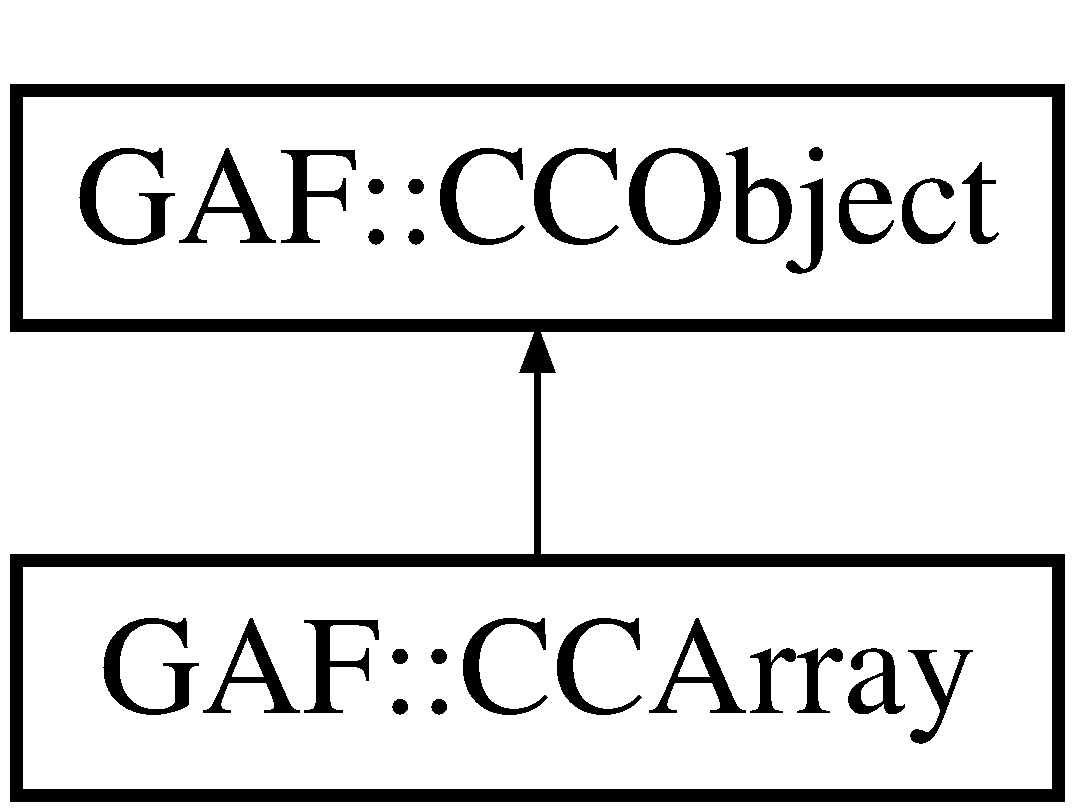
\includegraphics[height=2.000000cm]{class_g_a_f_1_1_c_c_array}
\end{center}
\end{figure}
\subsection*{Public Member Functions}
\begin{DoxyCompactItemize}
\item 
\hypertarget{class_g_a_f_1_1_c_c_array_a7fee3c1bfabcfcf7fa3f80511e9f2d3e}{unsigned int {\bfseries count} () const }\label{class_g_a_f_1_1_c_c_array_a7fee3c1bfabcfcf7fa3f80511e9f2d3e}

\item 
\hypertarget{class_g_a_f_1_1_c_c_array_ace44f70634187ea60d918c7d3a7ef971}{\hyperlink{class_g_a_f_1_1_c_c_object}{C\-C\-Object} $\ast$ {\bfseries last\-Object} ()}\label{class_g_a_f_1_1_c_c_array_ace44f70634187ea60d918c7d3a7ef971}

\item 
\hypertarget{class_g_a_f_1_1_c_c_array_a8ae859d22700439b031242fbe22c982d}{\hyperlink{class_g_a_f_1_1_c_c_object}{C\-C\-Object} $\ast$ {\bfseries object\-At\-Index} (unsigned int index)}\label{class_g_a_f_1_1_c_c_array_a8ae859d22700439b031242fbe22c982d}

\item 
\hypertarget{class_g_a_f_1_1_c_c_array_aa60d1a846fb8110a5f0720a6108d8de1}{void {\bfseries add\-Object} (\hyperlink{class_g_a_f_1_1_c_c_object}{C\-C\-Object} $\ast$object)}\label{class_g_a_f_1_1_c_c_array_aa60d1a846fb8110a5f0720a6108d8de1}

\item 
\hypertarget{class_g_a_f_1_1_c_c_array_a8131e3de0c1763c280a5446fce6432ab}{void {\bfseries remove\-All\-Objects} ()}\label{class_g_a_f_1_1_c_c_array_a8131e3de0c1763c280a5446fce6432ab}

\item 
\hypertarget{class_g_a_f_1_1_c_c_array_a6d4e35202989cf876fe8683652bc6352}{void {\bfseries remove\-Last\-Object} ()}\label{class_g_a_f_1_1_c_c_array_a6d4e35202989cf876fe8683652bc6352}

\item 
\hypertarget{class_g_a_f_1_1_c_c_array_a158b2114ddb9988588195bf9515cad7b}{void {\bfseries fast\-Remove\-Object\-At\-Index} (int index)}\label{class_g_a_f_1_1_c_c_array_a158b2114ddb9988588195bf9515cad7b}

\item 
\hypertarget{class_g_a_f_1_1_c_c_array_ae3c8354f2d5420781817303f0b61d097}{std\-::vector$<$ \hyperlink{class_g_a_f_1_1_c_c_object}{C\-C\-Object} $\ast$ $>$ \& {\bfseries vect} ()}\label{class_g_a_f_1_1_c_c_array_ae3c8354f2d5420781817303f0b61d097}

\end{DoxyCompactItemize}
\subsection*{Static Public Member Functions}
\begin{DoxyCompactItemize}
\item 
\hypertarget{class_g_a_f_1_1_c_c_array_a947a45d82f708788099f2e8dbcea2dd3}{static \hyperlink{class_g_a_f_1_1_c_c_array}{C\-C\-Array} $\ast$ {\bfseries create} ()}\label{class_g_a_f_1_1_c_c_array_a947a45d82f708788099f2e8dbcea2dd3}

\item 
\hypertarget{class_g_a_f_1_1_c_c_array_a247c90f7c332f7e49e950f297793d598}{static \hyperlink{class_g_a_f_1_1_c_c_array}{C\-C\-Array} $\ast$ {\bfseries create\-With\-Array} (\hyperlink{class_g_a_f_1_1_c_c_array}{C\-C\-Array} $\ast$array)}\label{class_g_a_f_1_1_c_c_array_a247c90f7c332f7e49e950f297793d598}

\item 
\hypertarget{class_g_a_f_1_1_c_c_array_a68779ee5b8c9e3e105b13016faf0298f}{static \hyperlink{class_g_a_f_1_1_c_c_array}{C\-C\-Array} $\ast$ {\bfseries create\-With\-Capacity} (int size)}\label{class_g_a_f_1_1_c_c_array_a68779ee5b8c9e3e105b13016faf0298f}

\end{DoxyCompactItemize}


\subsection{Detailed Description}
Internal class of G\-A\-F Marmalade Library. It is used for emulation of Cocos2dx A\-P\-I and envirmonment for the Library. The purpose of the class is to have A\-P\-I that match A\-P\-I of Cocos2dx object, but the class itself has minimal set of features. It does not depend on Cocos2dx. We use it to unify the code of G\-A\-F Libraries across the frameworks. All support classes are located in namespace G\-A\-F. In future G\-A\-F Marmalade can support new rendering backend (other than Cocos2dx), and the effort is made to minimize code differences between libraries. If you are going to use only Cocos2dx as rendering backend you do not have to use theese classes or even know about them. If you are planning to switch to new backend that G\-A\-F Marmalade will support you should not use any Cocos2dx class and instead use your own or classes from cocoagaf. If you need reference counting compatible with any of future releases you should use \hyperlink{class_g_a_f_1_1_c_c_object}{G\-A\-F\-::\-C\-C\-Object} as well. 

The documentation for this class was generated from the following file\-:\begin{DoxyCompactItemize}
\item 
cocoagaf/G\-A\-F\-Array.\-h\end{DoxyCompactItemize}

\hypertarget{class_g_a_f_1_1_c_c_bool}{\section{G\-A\-F\-:\-:C\-C\-Bool Class Reference}
\label{class_g_a_f_1_1_c_c_bool}\index{G\-A\-F\-::\-C\-C\-Bool@{G\-A\-F\-::\-C\-C\-Bool}}
}


{\ttfamily \#include $<$G\-A\-F\-Bool.\-h$>$}

Inheritance diagram for G\-A\-F\-:\-:C\-C\-Bool\-:\begin{figure}[H]
\begin{center}
\leavevmode
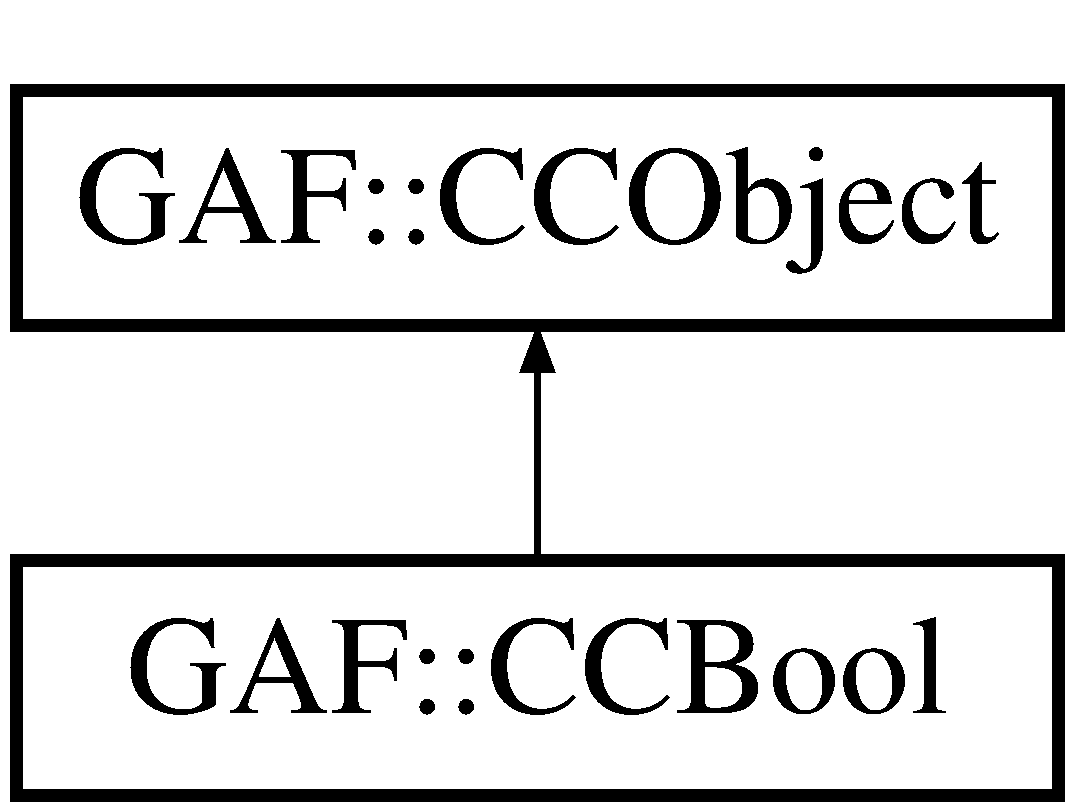
\includegraphics[height=2.000000cm]{class_g_a_f_1_1_c_c_bool}
\end{center}
\end{figure}
\subsection*{Public Member Functions}
\begin{DoxyCompactItemize}
\item 
\hypertarget{class_g_a_f_1_1_c_c_bool_aac86a418ff39a1e7b3df958bd3290449}{{\bfseries C\-C\-Bool} (bool value)}\label{class_g_a_f_1_1_c_c_bool_aac86a418ff39a1e7b3df958bd3290449}

\item 
\hypertarget{class_g_a_f_1_1_c_c_bool_a5a7a3cd1a9a5a67c25d76a7c4708e3b9}{bool {\bfseries get\-Value} () const }\label{class_g_a_f_1_1_c_c_bool_a5a7a3cd1a9a5a67c25d76a7c4708e3b9}

\item 
\hypertarget{class_g_a_f_1_1_c_c_bool_a3a5700928870a0f90097295836fd9542}{void {\bfseries set\-Value} (bool value)}\label{class_g_a_f_1_1_c_c_bool_a3a5700928870a0f90097295836fd9542}

\end{DoxyCompactItemize}
\subsection*{Static Public Member Functions}
\begin{DoxyCompactItemize}
\item 
\hypertarget{class_g_a_f_1_1_c_c_bool_ae52ca9fbf79812400ce0bc8aa8bb4984}{static \hyperlink{class_g_a_f_1_1_c_c_bool}{C\-C\-Bool} $\ast$ {\bfseries create} (bool v)}\label{class_g_a_f_1_1_c_c_bool_ae52ca9fbf79812400ce0bc8aa8bb4984}

\end{DoxyCompactItemize}


\subsection{Detailed Description}
Internal class of G\-A\-F Marmalade Library. It is used for emulation of Cocos2dx A\-P\-I and envirmonment for the Library. The purpose of the class is to have A\-P\-I that match A\-P\-I of Cocos2dx object, but the class itself has minimal set of features. It does not depend on Cocos2dx. We use it to unify the code of G\-A\-F Libraries across the frameworks. All support classes are located in namespace G\-A\-F. In future G\-A\-F Marmalade can support new rendering backend (other than Cocos2dx), and the effort is made to minimize code differences between libraries. If you are going to use only Cocos2dx as rendering backend you do not have to use theese classes or even know about them. If you are planning to switch to new backend that G\-A\-F Marmalade will support you should not use any Cocos2dx class and instead use your own or classes from cocoagaf. If you need reference counting compatible with any of future releases you should use \hyperlink{class_g_a_f_1_1_c_c_object}{G\-A\-F\-::\-C\-C\-Object} as well. 

The documentation for this class was generated from the following file\-:\begin{DoxyCompactItemize}
\item 
cocoagaf/G\-A\-F\-Bool.\-h\end{DoxyCompactItemize}

\hypertarget{class_g_a_f_1_1_c_c_dictionary}{\section{G\-A\-F\-:\-:C\-C\-Dictionary Class Reference}
\label{class_g_a_f_1_1_c_c_dictionary}\index{G\-A\-F\-::\-C\-C\-Dictionary@{G\-A\-F\-::\-C\-C\-Dictionary}}
}
Inheritance diagram for G\-A\-F\-:\-:C\-C\-Dictionary\-:\begin{figure}[H]
\begin{center}
\leavevmode
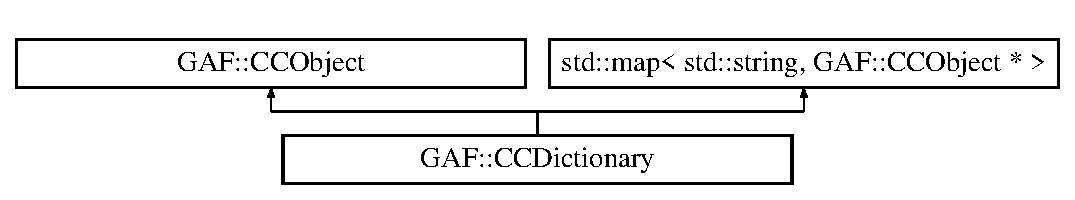
\includegraphics[height=2.000000cm]{class_g_a_f_1_1_c_c_dictionary}
\end{center}
\end{figure}
\subsection*{Public Member Functions}
\begin{DoxyCompactItemize}
\item 
\hypertarget{class_g_a_f_1_1_c_c_dictionary_a87a75f694d826abeb45451832714973e}{\hyperlink{class_g_a_f_1_1_c_c_object}{C\-C\-Object} $\ast$ {\bfseries object\-For\-Key} (const std\-::string \&key)}\label{class_g_a_f_1_1_c_c_dictionary_a87a75f694d826abeb45451832714973e}

\item 
\hypertarget{class_g_a_f_1_1_c_c_dictionary_a43d5b140a991edf12261fa4eaa849180}{unsigned int {\bfseries count} () const }\label{class_g_a_f_1_1_c_c_dictionary_a43d5b140a991edf12261fa4eaa849180}

\item 
\hypertarget{class_g_a_f_1_1_c_c_dictionary_a1830bfd69de9d6cfb0791e0c949e65bf}{void {\bfseries set\-Object} (\hyperlink{class_g_a_f_1_1_c_c_object}{C\-C\-Object} $\ast$object, const std\-::string \&key)}\label{class_g_a_f_1_1_c_c_dictionary_a1830bfd69de9d6cfb0791e0c949e65bf}

\item 
\hypertarget{class_g_a_f_1_1_c_c_dictionary_a469d957a35b3cd4441809e220e2463f8}{void {\bfseries remove\-All\-Objects} ()}\label{class_g_a_f_1_1_c_c_dictionary_a469d957a35b3cd4441809e220e2463f8}

\item 
\hypertarget{class_g_a_f_1_1_c_c_dictionary_a10310a3d3a87647dbfc2b33348b0a33e}{void {\bfseries remove\-Object\-For\-Key} (const std\-::string \&key)}\label{class_g_a_f_1_1_c_c_dictionary_a10310a3d3a87647dbfc2b33348b0a33e}

\item 
\hypertarget{class_g_a_f_1_1_c_c_dictionary_a2acc9819bce13b2ac2c93ff9eab800aa}{\hyperlink{class_g_a_f_1_1_c_c_array}{C\-C\-Array} $\ast$ {\bfseries all\-Keys} ()}\label{class_g_a_f_1_1_c_c_dictionary_a2acc9819bce13b2ac2c93ff9eab800aa}

\end{DoxyCompactItemize}
\subsection*{Static Public Member Functions}
\begin{DoxyCompactItemize}
\item 
\hypertarget{class_g_a_f_1_1_c_c_dictionary_a2496598cd2863df0920eea866a71312f}{static \hyperlink{class_g_a_f_1_1_c_c_dictionary}{C\-C\-Dictionary} $\ast$ {\bfseries create} ()}\label{class_g_a_f_1_1_c_c_dictionary_a2496598cd2863df0920eea866a71312f}

\end{DoxyCompactItemize}


The documentation for this class was generated from the following file\-:\begin{DoxyCompactItemize}
\item 
cocoagaf/G\-A\-F\-Dictionary.\-h\end{DoxyCompactItemize}

\hypertarget{class_g_a_f_1_1_c_c_image}{\section{G\-A\-F\-:\-:C\-C\-Image Class Reference}
\label{class_g_a_f_1_1_c_c_image}\index{G\-A\-F\-::\-C\-C\-Image@{G\-A\-F\-::\-C\-C\-Image}}
}


{\ttfamily \#include $<$G\-A\-F\-Image.\-h$>$}

Inheritance diagram for G\-A\-F\-:\-:C\-C\-Image\-:\begin{figure}[H]
\begin{center}
\leavevmode
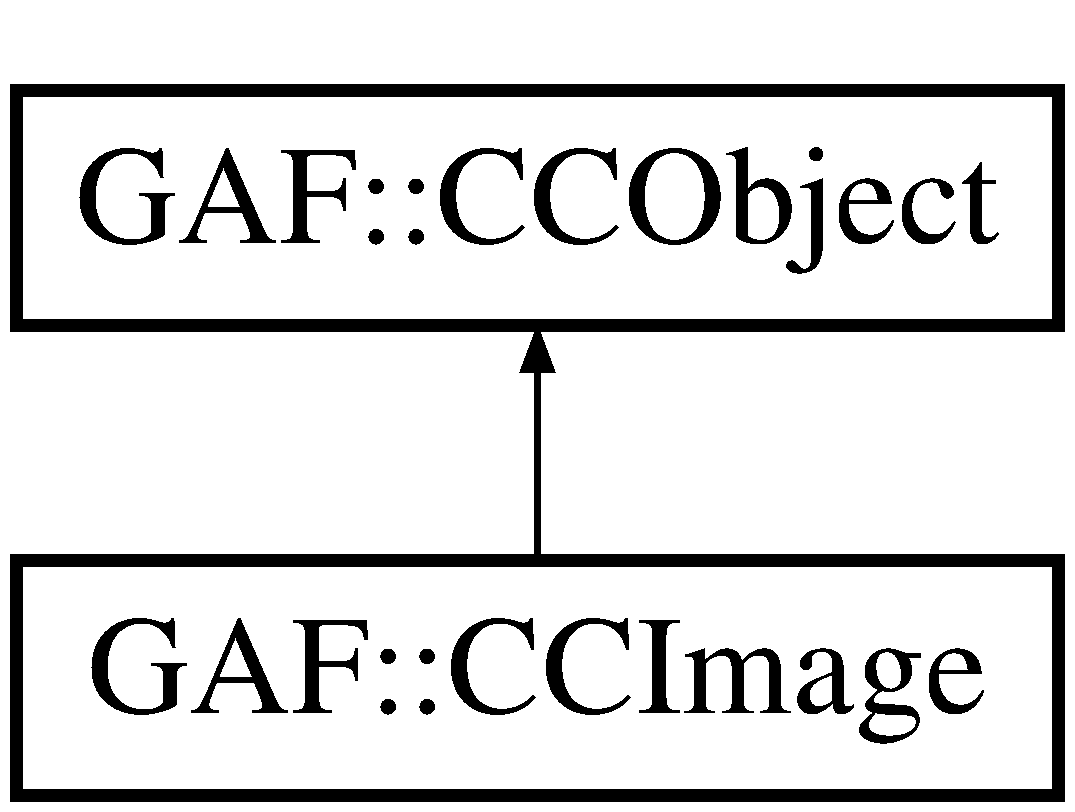
\includegraphics[height=2.000000cm]{class_g_a_f_1_1_c_c_image}
\end{center}
\end{figure}
\subsection*{Public Member Functions}
\begin{DoxyCompactItemize}
\item 
void $\ast$ \hyperlink{class_g_a_f_1_1_c_c_image_ab17ab53d6808ce7ebe8c3f3c5dd60e6a}{get\-External\-Pointer} () const 
\item 
\hypertarget{class_g_a_f_1_1_c_c_image_a7559bbec034c045ce0093c9d2bdc668e}{bool {\bfseries init\-With\-Image\-File} (const char $\ast$path)}\label{class_g_a_f_1_1_c_c_image_a7559bbec034c045ce0093c9d2bdc668e}

\end{DoxyCompactItemize}
\subsection*{Static Public Member Functions}
\begin{DoxyCompactItemize}
\item 
\hypertarget{class_g_a_f_1_1_c_c_image_a1ce843bd6d475a5cfb46db4218bbf515}{static \hyperlink{class_g_a_f_1_1_c_c_image}{C\-C\-Image} $\ast$ {\bfseries create} ()}\label{class_g_a_f_1_1_c_c_image_a1ce843bd6d475a5cfb46db4218bbf515}

\end{DoxyCompactItemize}


\subsection{Detailed Description}
Internal class of G\-A\-F Marmalade Library. It is used for emulation of Cocos2dx A\-P\-I and envirmonment for the Library. The purpose of the class is to have A\-P\-I that match A\-P\-I of Cocos2dx object, but the class itself has minimal set of features. It does not depend on Cocos2dx. We use it to unify the code of G\-A\-F Libraries across the frameworks. All support classes are located in namespace G\-A\-F. In future G\-A\-F Marmalade can support new rendering backend (other than Cocos2dx), and the effort is made to minimize code differences between libraries. If you are going to use only Cocos2dx as rendering backend you do not have to use theese classes or even know about them. If you are planning to switch to new backend that G\-A\-F Marmalade will support you should not use any Cocos2dx class and instead use your own or classes from cocoagaf. If you need reference counting compatible with any of future releases you should use \hyperlink{class_g_a_f_1_1_c_c_object}{G\-A\-F\-::\-C\-C\-Object} as well. 

\subsection{Member Function Documentation}
\hypertarget{class_g_a_f_1_1_c_c_image_ab17ab53d6808ce7ebe8c3f3c5dd60e6a}{\index{G\-A\-F\-::\-C\-C\-Image@{G\-A\-F\-::\-C\-C\-Image}!get\-External\-Pointer@{get\-External\-Pointer}}
\index{get\-External\-Pointer@{get\-External\-Pointer}!GAF::CCImage@{G\-A\-F\-::\-C\-C\-Image}}
\subsubsection[{get\-External\-Pointer}]{\setlength{\rightskip}{0pt plus 5cm}void$\ast$ G\-A\-F\-::\-C\-C\-Image\-::get\-External\-Pointer (
\begin{DoxyParamCaption}
{}
\end{DoxyParamCaption}
) const\hspace{0.3cm}{\ttfamily [inline]}}}\label{class_g_a_f_1_1_c_c_image_ab17ab53d6808ce7ebe8c3f3c5dd60e6a}
\begin{DoxyReturn}{Returns}
external pointer to G\-A\-F rendering backend object 
\end{DoxyReturn}


The documentation for this class was generated from the following file\-:\begin{DoxyCompactItemize}
\item 
cocoagaf/G\-A\-F\-Image.\-h\end{DoxyCompactItemize}

\hypertarget{class_g_a_f_1_1_c_c_integer}{\section{G\-A\-F\-:\-:C\-C\-Integer Class Reference}
\label{class_g_a_f_1_1_c_c_integer}\index{G\-A\-F\-::\-C\-C\-Integer@{G\-A\-F\-::\-C\-C\-Integer}}
}


{\ttfamily \#include $<$G\-A\-F\-Integer.\-h$>$}

Inheritance diagram for G\-A\-F\-:\-:C\-C\-Integer\-:\begin{figure}[H]
\begin{center}
\leavevmode
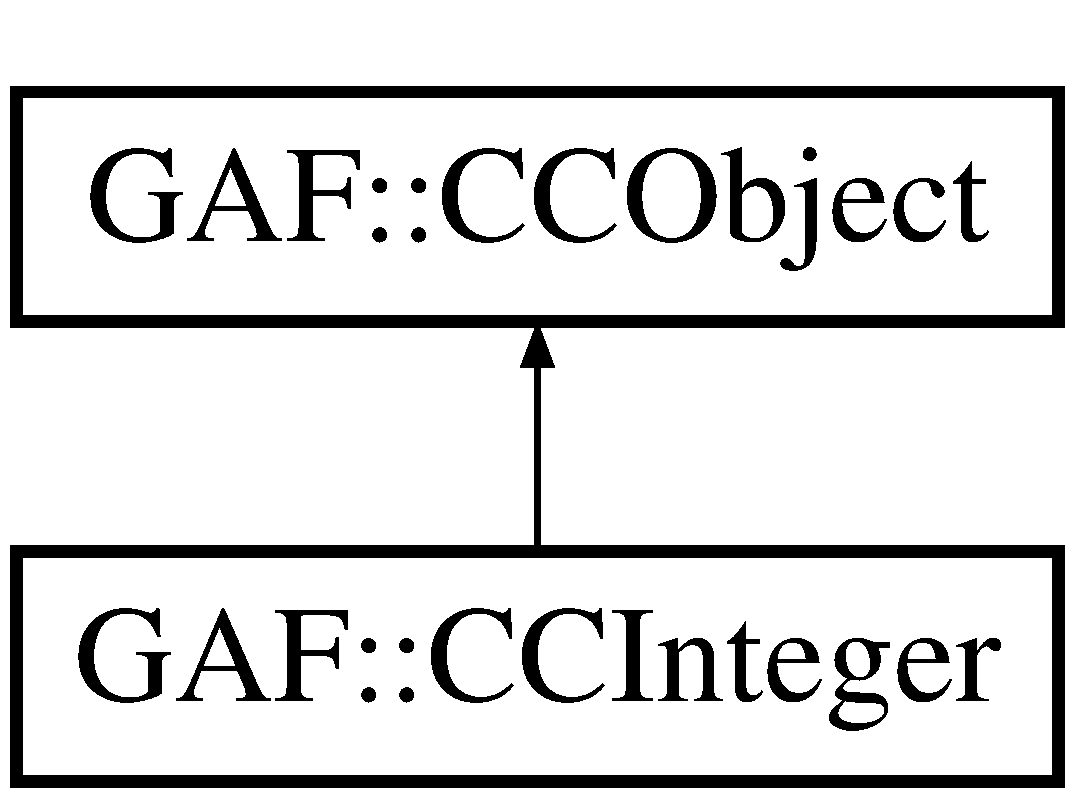
\includegraphics[height=2.000000cm]{class_g_a_f_1_1_c_c_integer}
\end{center}
\end{figure}
\subsection*{Public Member Functions}
\begin{DoxyCompactItemize}
\item 
\hypertarget{class_g_a_f_1_1_c_c_integer_a2793183f4108e22c85304580de6afef5}{int {\bfseries get\-Value} () const }\label{class_g_a_f_1_1_c_c_integer_a2793183f4108e22c85304580de6afef5}

\end{DoxyCompactItemize}
\subsection*{Static Public Member Functions}
\begin{DoxyCompactItemize}
\item 
\hypertarget{class_g_a_f_1_1_c_c_integer_ac058cd074ca1775881517852062ac76c}{static \hyperlink{class_g_a_f_1_1_c_c_integer}{C\-C\-Integer} $\ast$ {\bfseries create} (int v)}\label{class_g_a_f_1_1_c_c_integer_ac058cd074ca1775881517852062ac76c}

\end{DoxyCompactItemize}
\subsection*{Protected Member Functions}
\begin{DoxyCompactItemize}
\item 
\hypertarget{class_g_a_f_1_1_c_c_integer_a76cb2dc5a038b0fd847748b87cb53608}{{\bfseries C\-C\-Integer} (int v)}\label{class_g_a_f_1_1_c_c_integer_a76cb2dc5a038b0fd847748b87cb53608}

\end{DoxyCompactItemize}


\subsection{Detailed Description}
Internal class of G\-A\-F Marmalade Library. It is used for emulation of Cocos2dx A\-P\-I and envirmonment for the Library. The purpose of the class is to have A\-P\-I that match A\-P\-I of Cocos2dx object, but the class itself has minimal set of features. It does not depend on Cocos2dx. We use it to unify the code of G\-A\-F Libraries across the frameworks. All support classes are located in namespace G\-A\-F. In future G\-A\-F Marmalade can support new rendering backend (other than Cocos2dx), and the effort is made to minimize code differences between libraries. If you are going to use only Cocos2dx as rendering backend you do not have to use theese classes or even know about them. If you are planning to switch to new backend that G\-A\-F Marmalade will support you should not use any Cocos2dx class and instead use your own or classes from cocoagaf. If you need reference counting compatible with any of future releases you should use \hyperlink{class_g_a_f_1_1_c_c_object}{G\-A\-F\-::\-C\-C\-Object} as well. 

The documentation for this class was generated from the following file\-:\begin{DoxyCompactItemize}
\item 
cocoagaf/G\-A\-F\-Integer.\-h\end{DoxyCompactItemize}

\hypertarget{class_g_a_f_1_1_c_c_object}{\section{G\-A\-F\-:\-:C\-C\-Object Class Reference}
\label{class_g_a_f_1_1_c_c_object}\index{G\-A\-F\-::\-C\-C\-Object@{G\-A\-F\-::\-C\-C\-Object}}
}


{\ttfamily \#include $<$G\-A\-F\-Geometry.\-h$>$}

Inheritance diagram for G\-A\-F\-:\-:C\-C\-Object\-:\begin{figure}[H]
\begin{center}
\leavevmode
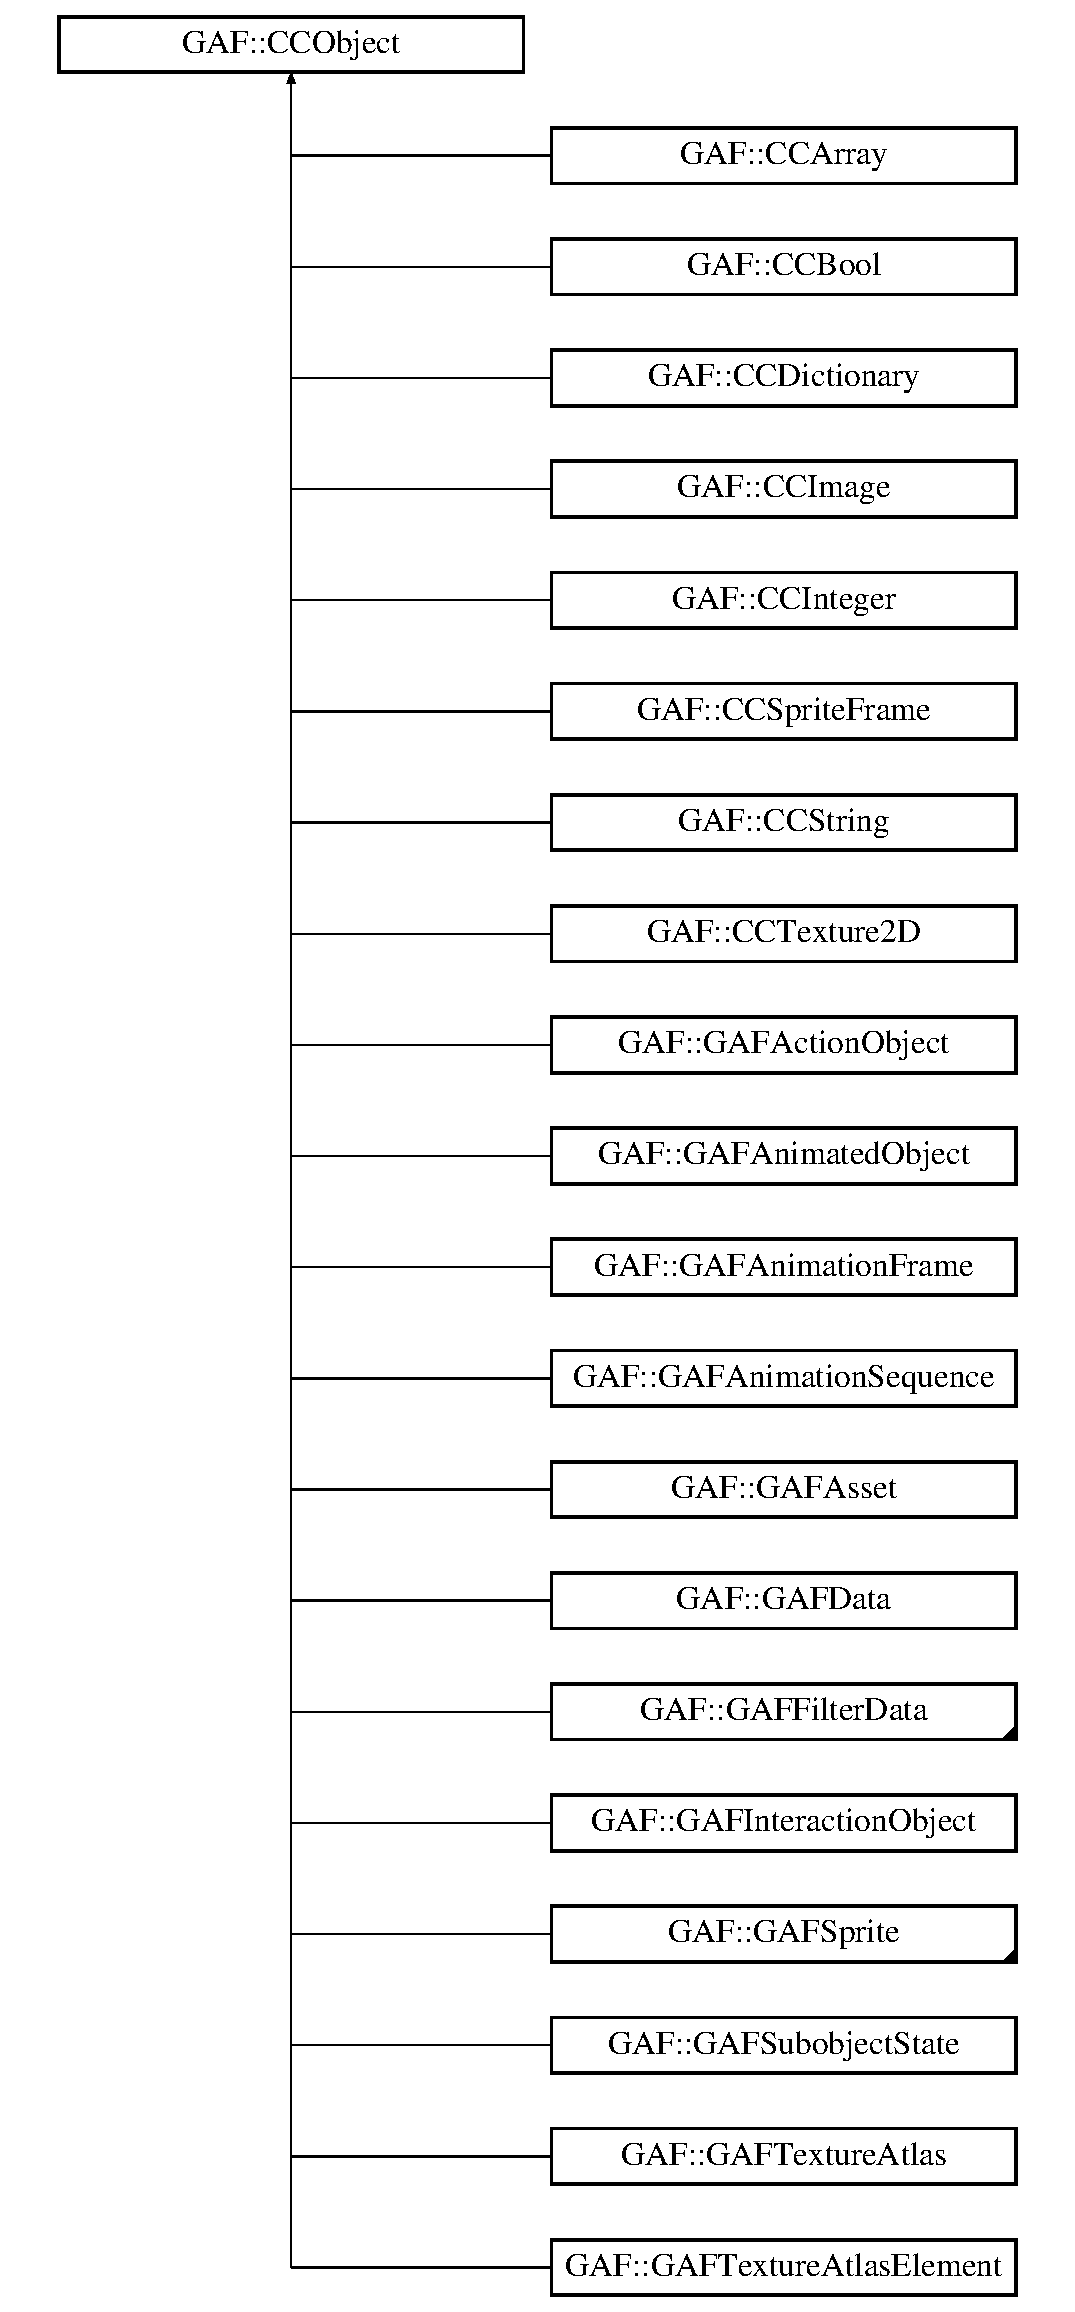
\includegraphics[height=12.000000cm]{class_g_a_f_1_1_c_c_object}
\end{center}
\end{figure}
\subsection*{Public Member Functions}
\begin{DoxyCompactItemize}
\item 
\hypertarget{class_g_a_f_1_1_c_c_object_a92d6be0cf04da2919e9039bef31f8584}{void {\bfseries retain} ()}\label{class_g_a_f_1_1_c_c_object_a92d6be0cf04da2919e9039bef31f8584}

\item 
\hypertarget{class_g_a_f_1_1_c_c_object_ab05fb1b3a8729e96ca23ddbe62c2d1c4}{void {\bfseries release} ()}\label{class_g_a_f_1_1_c_c_object_ab05fb1b3a8729e96ca23ddbe62c2d1c4}

\item 
\hypertarget{class_g_a_f_1_1_c_c_object_a4e3d530ba069913a6e5708ea3fbf2491}{\hyperlink{class_g_a_f_1_1_c_c_object}{C\-C\-Object} $\ast$ {\bfseries autorelease} ()}\label{class_g_a_f_1_1_c_c_object_a4e3d530ba069913a6e5708ea3fbf2491}

\item 
\hypertarget{class_g_a_f_1_1_c_c_object_ad2498666cde8606d0b113fca7a0ebf41}{void {\bfseries set\-User\-Data} (void $\ast$user\-Data)}\label{class_g_a_f_1_1_c_c_object_ad2498666cde8606d0b113fca7a0ebf41}

\item 
\hypertarget{class_g_a_f_1_1_c_c_object_adae0a97b469059ea1766bdc6eaf65c02}{void $\ast$ {\bfseries user\-Data} ()}\label{class_g_a_f_1_1_c_c_object_adae0a97b469059ea1766bdc6eaf65c02}

\item 
\hypertarget{class_g_a_f_1_1_c_c_object_a1bc5736a053deff185e344503a582ef8}{void {\bfseries set\-Tag} (int tag)}\label{class_g_a_f_1_1_c_c_object_a1bc5736a053deff185e344503a582ef8}

\item 
\hypertarget{class_g_a_f_1_1_c_c_object_ab5a4e313567c5c1e2791570385ba6873}{int {\bfseries get\-Tag} () const }\label{class_g_a_f_1_1_c_c_object_ab5a4e313567c5c1e2791570385ba6873}

\end{DoxyCompactItemize}


\subsection{Detailed Description}
Internal class of G\-A\-F Marmalade Library. It is used for emulation of Cocos2dx A\-P\-I and envirmonment for the Library. The purpose of the class is to have A\-P\-I that match A\-P\-I of Cocos2dx object, but the class itself has minimal set of features. It does not depend on Cocos2dx. We use it to unify the code of G\-A\-F Libraries across the frameworks. All support classes are located in namespace G\-A\-F. In future G\-A\-F Marmalade can support new rendering backend (other than Cocos2dx), and the effort is made to minimize code differences between libraries. If you are going to use only Cocos2dx as rendering backend you do not have to use theese classes or even know about them. If you are planning to switch to new backend that G\-A\-F Marmalade will support you should not use any Cocos2dx class and instead use your own or classes from cocoagaf. If you need reference counting compatible with any of future releases you should use \hyperlink{class_g_a_f_1_1_c_c_object}{G\-A\-F\-::\-C\-C\-Object} as well. 

The documentation for this class was generated from the following file\-:\begin{DoxyCompactItemize}
\item 
cocoagaf/G\-A\-F\-Object.\-h\end{DoxyCompactItemize}

\hypertarget{class_g_a_f_1_1_c_c_point}{\section{G\-A\-F\-:\-:C\-C\-Point Class Reference}
\label{class_g_a_f_1_1_c_c_point}\index{G\-A\-F\-::\-C\-C\-Point@{G\-A\-F\-::\-C\-C\-Point}}
}
\subsection*{Public Member Functions}
\begin{DoxyCompactItemize}
\item 
\hypertarget{class_g_a_f_1_1_c_c_point_aa4d9cdbb6f24e6f808a0e9fe2d4e61a3}{{\bfseries C\-C\-Point} (float \-\_\-x, float \-\_\-y)}\label{class_g_a_f_1_1_c_c_point_aa4d9cdbb6f24e6f808a0e9fe2d4e61a3}

\end{DoxyCompactItemize}
\subsection*{Public Attributes}
\begin{DoxyCompactItemize}
\item 
\hypertarget{class_g_a_f_1_1_c_c_point_ac90f32d335c2329da2797d0ed87b901a}{float {\bfseries x}}\label{class_g_a_f_1_1_c_c_point_ac90f32d335c2329da2797d0ed87b901a}

\item 
\hypertarget{class_g_a_f_1_1_c_c_point_a11bffcec6c48c0090443a23de93cb431}{float {\bfseries y}}\label{class_g_a_f_1_1_c_c_point_a11bffcec6c48c0090443a23de93cb431}

\end{DoxyCompactItemize}


The documentation for this class was generated from the following file\-:\begin{DoxyCompactItemize}
\item 
cocoagaf/G\-A\-F\-Geometry.\-h\end{DoxyCompactItemize}

\hypertarget{class_g_a_f_1_1_c_c_rect}{\section{G\-A\-F\-:\-:C\-C\-Rect Class Reference}
\label{class_g_a_f_1_1_c_c_rect}\index{G\-A\-F\-::\-C\-C\-Rect@{G\-A\-F\-::\-C\-C\-Rect}}
}


{\ttfamily \#include $<$G\-A\-F\-Geometry.\-h$>$}

\subsection*{Public Member Functions}
\begin{DoxyCompactItemize}
\item 
\hypertarget{class_g_a_f_1_1_c_c_rect_ac98d154bec883ca32305aeedf240395d}{{\bfseries C\-C\-Rect} (float x, float y, float width, float height)}\label{class_g_a_f_1_1_c_c_rect_ac98d154bec883ca32305aeedf240395d}

\end{DoxyCompactItemize}
\subsection*{Public Attributes}
\begin{DoxyCompactItemize}
\item 
\hypertarget{class_g_a_f_1_1_c_c_rect_ab4e03f6d8228bd9078c5c42670f7f020}{\hyperlink{class_g_a_f_1_1_c_c_point}{C\-C\-Point} {\bfseries origin}}\label{class_g_a_f_1_1_c_c_rect_ab4e03f6d8228bd9078c5c42670f7f020}

\item 
\hypertarget{class_g_a_f_1_1_c_c_rect_a6a766309814b1a2970f86ea3952a7587}{\hyperlink{class_g_a_f_1_1_c_c_size}{C\-C\-Size} {\bfseries size}}\label{class_g_a_f_1_1_c_c_rect_a6a766309814b1a2970f86ea3952a7587}

\end{DoxyCompactItemize}


\subsection{Detailed Description}
Internal class of G\-A\-F Marmalade Library. It is used for emulation of Cocos2dx A\-P\-I and envirmonment for the Library. The purpose of the class is to have A\-P\-I that match A\-P\-I of Cocos2dx object, but the class itself has minimal set of features. It does not depend on Cocos2dx. We use it to unify the code of G\-A\-F Libraries across the frameworks. All support classes are located in namespace G\-A\-F. In future G\-A\-F Marmalade can support new rendering backend (other than Cocos2dx), and the effort is made to minimize code differences between libraries. If you are going to use only Cocos2dx as rendering backend you do not have to use theese classes or even know about them. If you are planning to switch to new backend that G\-A\-F Marmalade will support you should not use any Cocos2dx class and instead use your own or classes from cocoagaf. If you need reference counting compatible with any of future releases you should use \hyperlink{class_g_a_f_1_1_c_c_object}{G\-A\-F\-::\-C\-C\-Object} as well. 

The documentation for this class was generated from the following file\-:\begin{DoxyCompactItemize}
\item 
cocoagaf/G\-A\-F\-Geometry.\-h\end{DoxyCompactItemize}

\hypertarget{class_g_a_f_1_1_c_c_size}{\section{G\-A\-F\-:\-:C\-C\-Size Class Reference}
\label{class_g_a_f_1_1_c_c_size}\index{G\-A\-F\-::\-C\-C\-Size@{G\-A\-F\-::\-C\-C\-Size}}
}


{\ttfamily \#include $<$G\-A\-F\-Geometry.\-h$>$}

\subsection*{Public Member Functions}
\begin{DoxyCompactItemize}
\item 
\hypertarget{class_g_a_f_1_1_c_c_size_a2ed4bb237cf3db7d19c4c403131dacd7}{{\bfseries C\-C\-Size} (float w, float h)}\label{class_g_a_f_1_1_c_c_size_a2ed4bb237cf3db7d19c4c403131dacd7}

\end{DoxyCompactItemize}
\subsection*{Public Attributes}
\begin{DoxyCompactItemize}
\item 
\hypertarget{class_g_a_f_1_1_c_c_size_a957274761169e02e8af661268a71e8b5}{float {\bfseries width}}\label{class_g_a_f_1_1_c_c_size_a957274761169e02e8af661268a71e8b5}

\item 
\hypertarget{class_g_a_f_1_1_c_c_size_a273c0fe58e5f33ee858f71c48a597347}{float {\bfseries height}}\label{class_g_a_f_1_1_c_c_size_a273c0fe58e5f33ee858f71c48a597347}

\end{DoxyCompactItemize}


\subsection{Detailed Description}
Internal class of G\-A\-F Marmalade Library. It is used for emulation of Cocos2dx A\-P\-I and envirmonment for the Library. The purpose of the class is to have A\-P\-I that match A\-P\-I of Cocos2dx object, but the class itself has minimal set of features. It does not depend on Cocos2dx. We use it to unify the code of G\-A\-F Libraries across the frameworks. All support classes are located in namespace G\-A\-F. In future G\-A\-F Marmalade can support new rendering backend (other than Cocos2dx), and the effort is made to minimize code differences between libraries. If you are going to use only Cocos2dx as rendering backend you do not have to use theese classes or even know about them. If you are planning to switch to new backend that G\-A\-F Marmalade will support you should not use any Cocos2dx class and instead use your own or classes from cocoagaf. If you need reference counting compatible with any of future releases you should use \hyperlink{class_g_a_f_1_1_c_c_object}{G\-A\-F\-::\-C\-C\-Object} as well. 

The documentation for this class was generated from the following file\-:\begin{DoxyCompactItemize}
\item 
cocoagaf/G\-A\-F\-Geometry.\-h\end{DoxyCompactItemize}

\hypertarget{class_g_a_f_1_1_c_c_sprite_frame}{\section{G\-A\-F\-:\-:C\-C\-Sprite\-Frame Class Reference}
\label{class_g_a_f_1_1_c_c_sprite_frame}\index{G\-A\-F\-::\-C\-C\-Sprite\-Frame@{G\-A\-F\-::\-C\-C\-Sprite\-Frame}}
}


{\ttfamily \#include $<$G\-A\-F\-Sprite\-Frame.\-h$>$}

Inheritance diagram for G\-A\-F\-:\-:C\-C\-Sprite\-Frame\-:\begin{figure}[H]
\begin{center}
\leavevmode
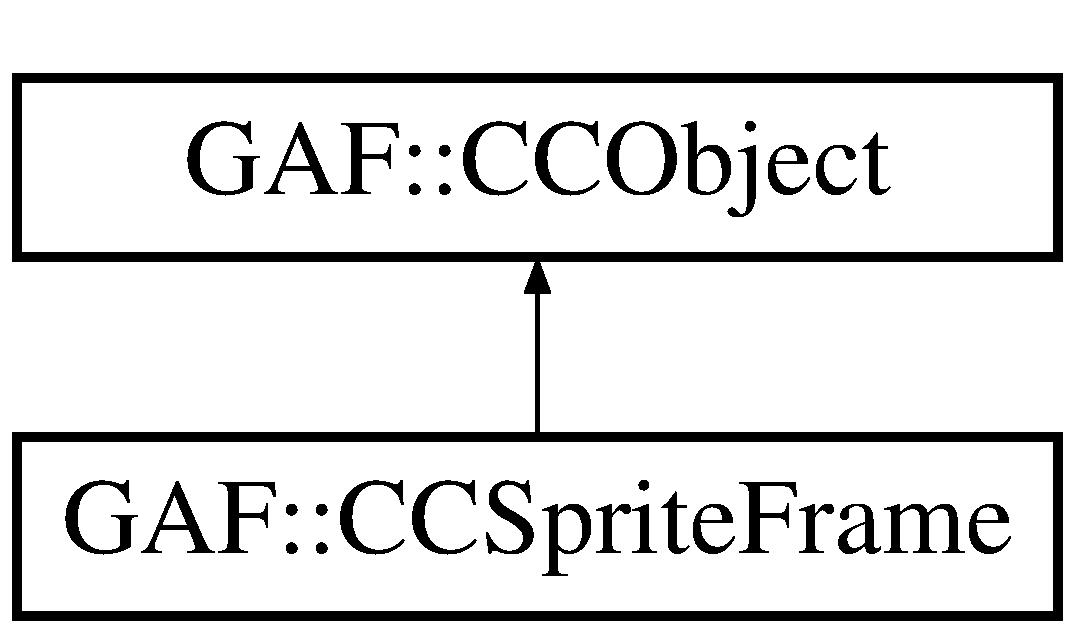
\includegraphics[height=2.000000cm]{class_g_a_f_1_1_c_c_sprite_frame}
\end{center}
\end{figure}
\subsection*{Public Member Functions}
\begin{DoxyCompactItemize}
\item 
void $\ast$ \hyperlink{class_g_a_f_1_1_c_c_sprite_frame_affaa9cf5921fd3ee39eed8e383948f87}{get\-External\-Pointer} ()
\end{DoxyCompactItemize}
\subsection*{Static Public Member Functions}
\begin{DoxyCompactItemize}
\item 
\hypertarget{class_g_a_f_1_1_c_c_sprite_frame_a64a7fb555d51aa998b64524e5e62433c}{static \hyperlink{class_g_a_f_1_1_c_c_sprite_frame}{C\-C\-Sprite\-Frame} $\ast$ {\bfseries create\-With\-Texture} (\hyperlink{class_g_a_f_1_1_c_c_texture2_d}{C\-C\-Texture2\-D} $\ast$pob\-Texture, const \hyperlink{class_g_a_f_1_1_c_c_rect}{C\-C\-Rect} \&rect)}\label{class_g_a_f_1_1_c_c_sprite_frame_a64a7fb555d51aa998b64524e5e62433c}

\end{DoxyCompactItemize}


\subsection{Detailed Description}
Internal class of G\-A\-F Marmalade Library. It is used for emulation of Cocos2dx A\-P\-I and envirmonment for the Library. The purpose of the class is to have A\-P\-I that match A\-P\-I of Cocos2dx object, but the class itself has minimal set of features. It does not depend on Cocos2dx. We use it to unify the code of G\-A\-F Libraries across the frameworks. All support classes are located in namespace G\-A\-F. In future G\-A\-F Marmalade can support new rendering backend (other than Cocos2dx), and the effort is made to minimize code differences between libraries. If you are going to use only Cocos2dx as rendering backend you do not have to use theese classes or even know about them. If you are planning to switch to new backend that G\-A\-F Marmalade will support you should not use any Cocos2dx class and instead use your own or classes from cocoagaf. If you need reference counting compatible with any of future releases you should use \hyperlink{class_g_a_f_1_1_c_c_object}{G\-A\-F\-::\-C\-C\-Object} as well. 

\subsection{Member Function Documentation}
\hypertarget{class_g_a_f_1_1_c_c_sprite_frame_affaa9cf5921fd3ee39eed8e383948f87}{\index{G\-A\-F\-::\-C\-C\-Sprite\-Frame@{G\-A\-F\-::\-C\-C\-Sprite\-Frame}!get\-External\-Pointer@{get\-External\-Pointer}}
\index{get\-External\-Pointer@{get\-External\-Pointer}!GAF::CCSpriteFrame@{G\-A\-F\-::\-C\-C\-Sprite\-Frame}}
\subsubsection[{get\-External\-Pointer}]{\setlength{\rightskip}{0pt plus 5cm}void$\ast$ G\-A\-F\-::\-C\-C\-Sprite\-Frame\-::get\-External\-Pointer (
\begin{DoxyParamCaption}
{}
\end{DoxyParamCaption}
)\hspace{0.3cm}{\ttfamily [inline]}}}\label{class_g_a_f_1_1_c_c_sprite_frame_affaa9cf5921fd3ee39eed8e383948f87}
\begin{DoxyReturn}{Returns}
external pointer to G\-A\-F rendering backend object 
\end{DoxyReturn}


The documentation for this class was generated from the following file\-:\begin{DoxyCompactItemize}
\item 
cocoagaf/G\-A\-F\-Sprite\-Frame.\-h\end{DoxyCompactItemize}

\hypertarget{class_g_a_f_1_1_c_c_string}{\section{G\-A\-F\-:\-:C\-C\-String Class Reference}
\label{class_g_a_f_1_1_c_c_string}\index{G\-A\-F\-::\-C\-C\-String@{G\-A\-F\-::\-C\-C\-String}}
}


{\ttfamily \#include $<$G\-A\-F\-String.\-h$>$}

Inheritance diagram for G\-A\-F\-:\-:C\-C\-String\-:\begin{figure}[H]
\begin{center}
\leavevmode
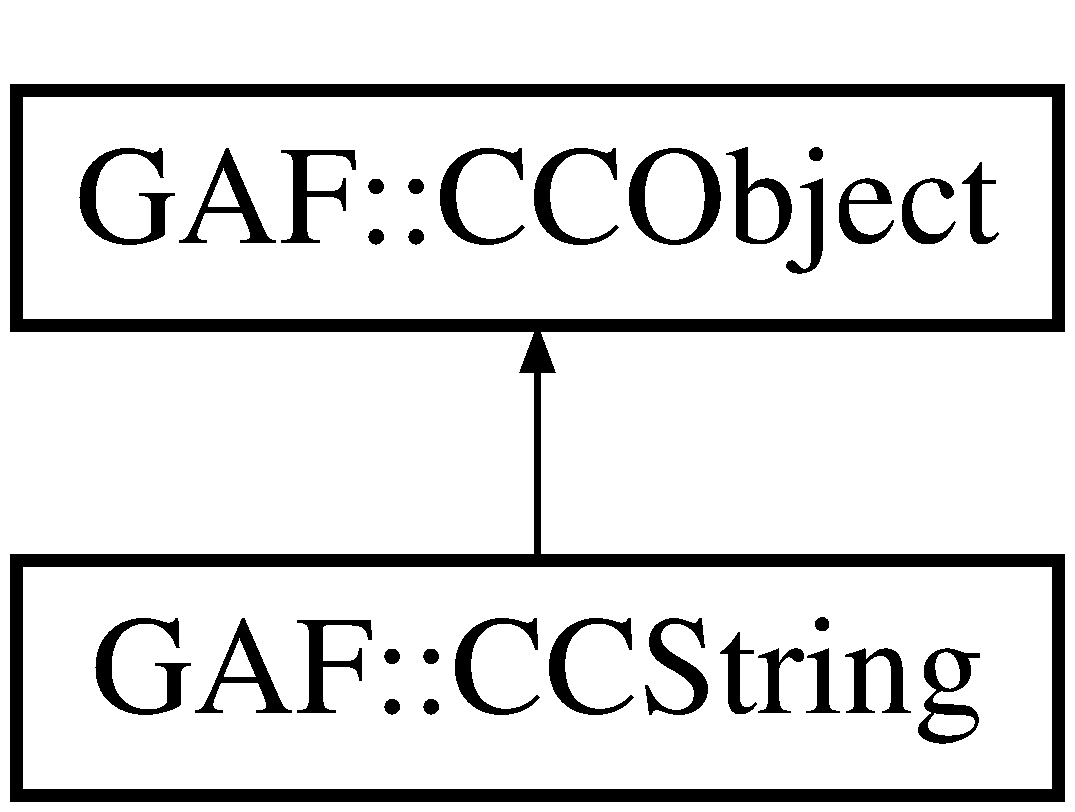
\includegraphics[height=2.000000cm]{class_g_a_f_1_1_c_c_string}
\end{center}
\end{figure}
\subsection*{Public Member Functions}
\begin{DoxyCompactItemize}
\item 
\hypertarget{class_g_a_f_1_1_c_c_string_acb10c8d19397ba78338e04c86928af74}{const char $\ast$ {\bfseries get\-C\-String} () const }\label{class_g_a_f_1_1_c_c_string_acb10c8d19397ba78338e04c86928af74}

\item 
\hypertarget{class_g_a_f_1_1_c_c_string_a3a69d5ee2fdd5230bf80cd52269c49ea}{{\bfseries C\-C\-String} (const char $\ast$str)}\label{class_g_a_f_1_1_c_c_string_a3a69d5ee2fdd5230bf80cd52269c49ea}

\item 
\hypertarget{class_g_a_f_1_1_c_c_string_a77a770c1de66847d3706433a5a331ea6}{{\bfseries C\-C\-String} (const std\-::string \&str)}\label{class_g_a_f_1_1_c_c_string_a77a770c1de66847d3706433a5a331ea6}

\end{DoxyCompactItemize}
\subsection*{Static Public Member Functions}
\begin{DoxyCompactItemize}
\item 
\hypertarget{class_g_a_f_1_1_c_c_string_a7bdc8ceafa9da8f5f5f11c57c582ddbb}{static \hyperlink{class_g_a_f_1_1_c_c_string}{C\-C\-String} $\ast$ {\bfseries create} (const char $\ast$str)}\label{class_g_a_f_1_1_c_c_string_a7bdc8ceafa9da8f5f5f11c57c582ddbb}

\item 
\hypertarget{class_g_a_f_1_1_c_c_string_a36edb4b0a30039f240f7057ff8d1448a}{static \hyperlink{class_g_a_f_1_1_c_c_string}{C\-C\-String} $\ast$ {\bfseries create} (const std\-::string \&str)}\label{class_g_a_f_1_1_c_c_string_a36edb4b0a30039f240f7057ff8d1448a}

\end{DoxyCompactItemize}


\subsection{Detailed Description}
Internal class of G\-A\-F Marmalade Library. It is used for emulation of Cocos2dx A\-P\-I and envirmonment for the Library. The purpose of the class is to have A\-P\-I that match A\-P\-I of Cocos2dx object, but the class itself has minimal set of features. It does not depend on Cocos2dx. We use it to unify the code of G\-A\-F Libraries across the frameworks. All support classes are located in namespace G\-A\-F. In future G\-A\-F Marmalade can support new rendering backend (other than Cocos2dx), and the effort is made to minimize code differences between libraries. If you are going to use only Cocos2dx as rendering backend you do not have to use theese classes or even know about them. If you are planning to switch to new backend that G\-A\-F Marmalade will support you should not use any Cocos2dx class and instead use your own or classes from cocoagaf. If you need reference counting compatible with any of future releases you should use \hyperlink{class_g_a_f_1_1_c_c_object}{G\-A\-F\-::\-C\-C\-Object} as well. 

The documentation for this class was generated from the following file\-:\begin{DoxyCompactItemize}
\item 
cocoagaf/G\-A\-F\-String.\-h\end{DoxyCompactItemize}

\hypertarget{class_g_a_f_1_1_c_c_texture2_d}{\section{G\-A\-F\-:\-:C\-C\-Texture2\-D Class Reference}
\label{class_g_a_f_1_1_c_c_texture2_d}\index{G\-A\-F\-::\-C\-C\-Texture2\-D@{G\-A\-F\-::\-C\-C\-Texture2\-D}}
}


{\ttfamily \#include $<$G\-A\-F\-Texture.\-h$>$}

Inheritance diagram for G\-A\-F\-:\-:C\-C\-Texture2\-D\-:\begin{figure}[H]
\begin{center}
\leavevmode
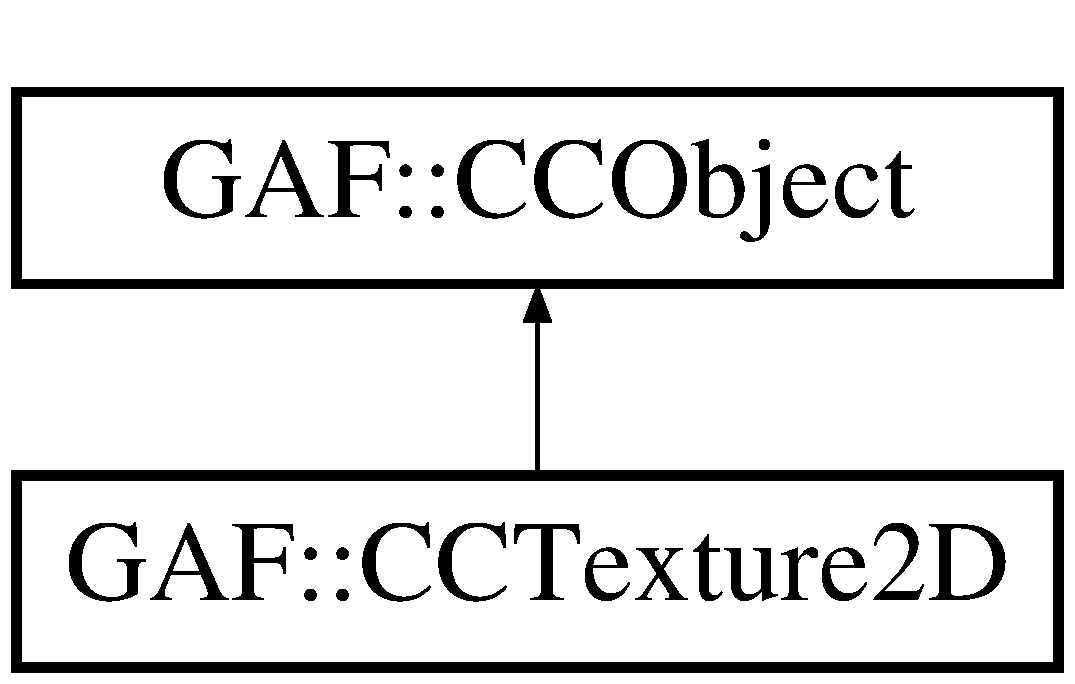
\includegraphics[height=2.000000cm]{class_g_a_f_1_1_c_c_texture2_d}
\end{center}
\end{figure}
\subsection*{Public Member Functions}
\begin{DoxyCompactItemize}
\item 
\hypertarget{class_g_a_f_1_1_c_c_texture2_d_af3b2b7faeb932e796ffd249041843236}{bool {\bfseries init\-With\-Image} (\hyperlink{class_g_a_f_1_1_c_c_image}{C\-C\-Image} $\ast$image)}\label{class_g_a_f_1_1_c_c_texture2_d_af3b2b7faeb932e796ffd249041843236}

\item 
void $\ast$ \hyperlink{class_g_a_f_1_1_c_c_texture2_d_ac0ae70bb23eacafb6947028779fbc456}{get\-External\-Pointer} ()
\end{DoxyCompactItemize}
\subsection*{Static Public Member Functions}
\begin{DoxyCompactItemize}
\item 
\hypertarget{class_g_a_f_1_1_c_c_texture2_d_a0a962928653419eb50f7f004af35bdd8}{static \hyperlink{class_g_a_f_1_1_c_c_texture2_d}{C\-C\-Texture2\-D} $\ast$ {\bfseries create} ()}\label{class_g_a_f_1_1_c_c_texture2_d_a0a962928653419eb50f7f004af35bdd8}

\end{DoxyCompactItemize}


\subsection{Detailed Description}
Internal class of G\-A\-F Marmalade Library. It is used for emulation of Cocos2dx A\-P\-I and envirmonment for the Library. The purpose of the class is to have A\-P\-I that match A\-P\-I of Cocos2dx object, but the class itself has minimal set of features. It does not depend on Cocos2dx. We use it to unify the code of G\-A\-F Libraries across the frameworks. All support classes are located in namespace G\-A\-F. In future G\-A\-F Marmalade can support new rendering backend (other than Cocos2dx), and the effort is made to minimize code differences between libraries. If you are going to use only Cocos2dx as rendering backend you do not have to use theese classes or even know about them. If you are planning to switch to new backend that G\-A\-F Marmalade will support you should not use any Cocos2dx class and instead use your own or classes from cocoagaf. If you need reference counting compatible with any of future releases you should use \hyperlink{class_g_a_f_1_1_c_c_object}{G\-A\-F\-::\-C\-C\-Object} as well. 

\subsection{Member Function Documentation}
\hypertarget{class_g_a_f_1_1_c_c_texture2_d_ac0ae70bb23eacafb6947028779fbc456}{\index{G\-A\-F\-::\-C\-C\-Texture2\-D@{G\-A\-F\-::\-C\-C\-Texture2\-D}!get\-External\-Pointer@{get\-External\-Pointer}}
\index{get\-External\-Pointer@{get\-External\-Pointer}!GAF::CCTexture2D@{G\-A\-F\-::\-C\-C\-Texture2\-D}}
\subsubsection[{get\-External\-Pointer}]{\setlength{\rightskip}{0pt plus 5cm}void$\ast$ G\-A\-F\-::\-C\-C\-Texture2\-D\-::get\-External\-Pointer (
\begin{DoxyParamCaption}
{}
\end{DoxyParamCaption}
)\hspace{0.3cm}{\ttfamily [inline]}}}\label{class_g_a_f_1_1_c_c_texture2_d_ac0ae70bb23eacafb6947028779fbc456}
\begin{DoxyReturn}{Returns}
external pointer to G\-A\-F rendering backend object 
\end{DoxyReturn}


The documentation for this class was generated from the following file\-:\begin{DoxyCompactItemize}
\item 
cocoagaf/G\-A\-F\-Texture.\-h\end{DoxyCompactItemize}

\hypertarget{class_g_a_f_1_1_g_a_f_action_object}{\section{G\-A\-F\-:\-:G\-A\-F\-Action\-Object Class Reference}
\label{class_g_a_f_1_1_g_a_f_action_object}\index{G\-A\-F\-::\-G\-A\-F\-Action\-Object@{G\-A\-F\-::\-G\-A\-F\-Action\-Object}}
}
Inheritance diagram for G\-A\-F\-:\-:G\-A\-F\-Action\-Object\-:\begin{figure}[H]
\begin{center}
\leavevmode
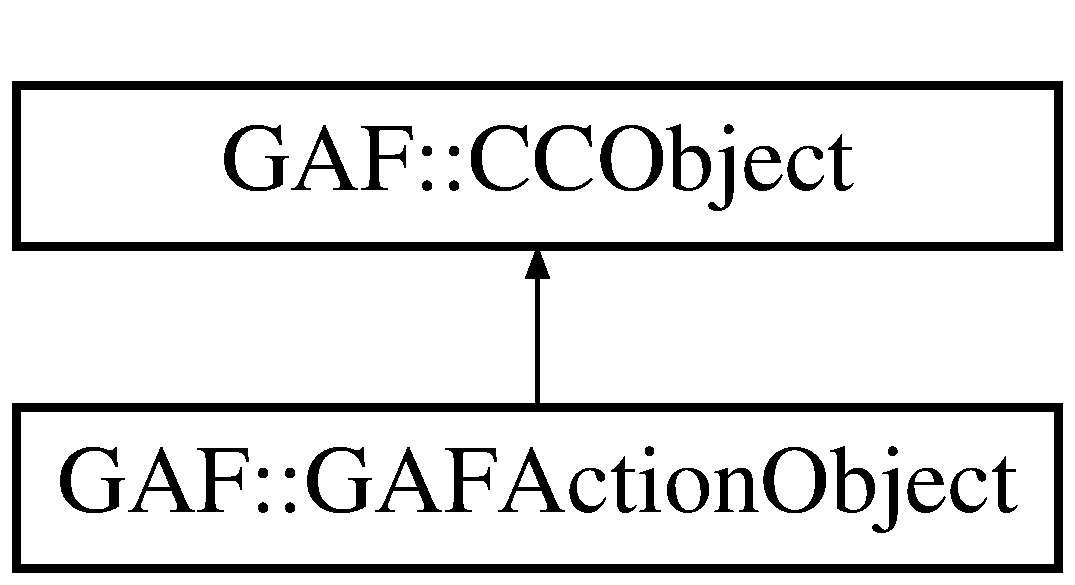
\includegraphics[height=2.000000cm]{class_g_a_f_1_1_g_a_f_action_object}
\end{center}
\end{figure}
\subsection*{Public Attributes}
\begin{DoxyCompactItemize}
\item 
std\-::string \hyperlink{class_g_a_f_1_1_g_a_f_action_object_a696f101b3aebdf344632e81a95224643}{name}
\item 
\hyperlink{class_g_a_f_1_1_c_c_point}{C\-C\-Point} \hyperlink{class_g_a_f_1_1_g_a_f_action_object_a01c42a4efc8e307d1e4ac799fffaedff}{pivot\-Point}
\item 
\hyperlink{class_g_a_f_1_1_c_c_rect}{C\-C\-Rect} \hyperlink{class_g_a_f_1_1_g_a_f_action_object_a9c0d295e1fb13ee4f6393bb08084565c}{bounds}
\end{DoxyCompactItemize}
\subsection*{Friends}
\begin{DoxyCompactItemize}
\item 
\hypertarget{class_g_a_f_1_1_g_a_f_action_object_adda4123c09612e8468a449e138c2f396}{class {\bfseries G\-A\-F\-Asset}}\label{class_g_a_f_1_1_g_a_f_action_object_adda4123c09612e8468a449e138c2f396}

\end{DoxyCompactItemize}
\subsection*{Additional Inherited Members}


\subsection{Member Data Documentation}
\hypertarget{class_g_a_f_1_1_g_a_f_action_object_a9c0d295e1fb13ee4f6393bb08084565c}{\index{G\-A\-F\-::\-G\-A\-F\-Action\-Object@{G\-A\-F\-::\-G\-A\-F\-Action\-Object}!bounds@{bounds}}
\index{bounds@{bounds}!GAF::GAFActionObject@{G\-A\-F\-::\-G\-A\-F\-Action\-Object}}
\subsubsection[{bounds}]{\setlength{\rightskip}{0pt plus 5cm}{\bf C\-C\-Rect} G\-A\-F\-::\-G\-A\-F\-Action\-Object\-::bounds}}\label{class_g_a_f_1_1_g_a_f_action_object_a9c0d295e1fb13ee4f6393bb08084565c}
Bounds of the object/subobject with respect to texture atlas. For advanced users only. \hypertarget{class_g_a_f_1_1_g_a_f_action_object_a696f101b3aebdf344632e81a95224643}{\index{G\-A\-F\-::\-G\-A\-F\-Action\-Object@{G\-A\-F\-::\-G\-A\-F\-Action\-Object}!name@{name}}
\index{name@{name}!GAF::GAFActionObject@{G\-A\-F\-::\-G\-A\-F\-Action\-Object}}
\subsubsection[{name}]{\setlength{\rightskip}{0pt plus 5cm}std\-::string G\-A\-F\-::\-G\-A\-F\-Action\-Object\-::name}}\label{class_g_a_f_1_1_g_a_f_action_object_a696f101b3aebdf344632e81a95224643}
Name of the object/subobject. You can query object/suboject by name in your application. \hypertarget{class_g_a_f_1_1_g_a_f_action_object_a01c42a4efc8e307d1e4ac799fffaedff}{\index{G\-A\-F\-::\-G\-A\-F\-Action\-Object@{G\-A\-F\-::\-G\-A\-F\-Action\-Object}!pivot\-Point@{pivot\-Point}}
\index{pivot\-Point@{pivot\-Point}!GAF::GAFActionObject@{G\-A\-F\-::\-G\-A\-F\-Action\-Object}}
\subsubsection[{pivot\-Point}]{\setlength{\rightskip}{0pt plus 5cm}{\bf C\-C\-Point} G\-A\-F\-::\-G\-A\-F\-Action\-Object\-::pivot\-Point}}\label{class_g_a_f_1_1_g_a_f_action_object_a01c42a4efc8e307d1e4ac799fffaedff}
Pivot point of the object/subobject with respect to object hierarchy. For advanced users only. 

The documentation for this class was generated from the following file\-:\begin{DoxyCompactItemize}
\item 
G\-A\-F\-Action\-Object.\-h\end{DoxyCompactItemize}

\hypertarget{class_g_a_f_1_1_g_a_f_animated_object}{\section{G\-A\-F\-:\-:G\-A\-F\-Animated\-Object Class Reference}
\label{class_g_a_f_1_1_g_a_f_animated_object}\index{G\-A\-F\-::\-G\-A\-F\-Animated\-Object@{G\-A\-F\-::\-G\-A\-F\-Animated\-Object}}
}
Inheritance diagram for G\-A\-F\-:\-:G\-A\-F\-Animated\-Object\-:\begin{figure}[H]
\begin{center}
\leavevmode
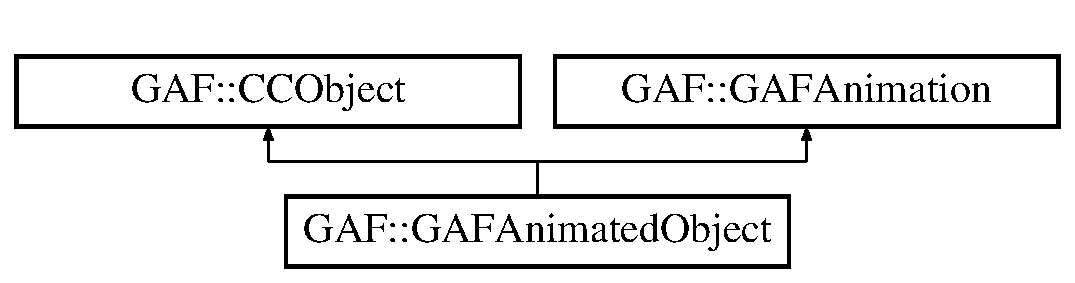
\includegraphics[height=2.000000cm]{class_g_a_f_1_1_g_a_f_animated_object}
\end{center}
\end{figure}
\subsection*{Public Member Functions}
\begin{DoxyCompactItemize}
\item 
\hypertarget{class_g_a_f_1_1_g_a_f_animated_object_a2d342145d85106586658123c42115f2d}{bool {\bfseries init} (\hyperlink{class_g_a_f_1_1_g_a_f_asset}{G\-A\-F\-Asset} $\ast$an\-Asset)}\label{class_g_a_f_1_1_g_a_f_animated_object_a2d342145d85106586658123c42115f2d}

\item 
\hypertarget{class_g_a_f_1_1_g_a_f_animated_object_abd1cb9fad4a76692f4ffb1a8dd699e31}{void {\bfseries process\-Animations} (float dt)}\label{class_g_a_f_1_1_g_a_f_animated_object_abd1cb9fad4a76692f4ffb1a8dd699e31}

\item 
\hypertarget{class_g_a_f_1_1_g_a_f_animated_object_afdc2654345e2e0bfed3297c709669bec}{\hyperlink{class_g_a_f_1_1_c_c_point}{C\-C\-Point} {\bfseries pupil\-Coordinates\-With\-X\-Semiaxis} (float an\-X\-Semiaxis, float an\-Y\-Semiaxis, \hyperlink{class_g_a_f_1_1_c_c_point}{C\-C\-Point} a\-Center, \hyperlink{class_g_a_f_1_1_c_c_point}{C\-C\-Point} an\-External\-Point)}\label{class_g_a_f_1_1_g_a_f_animated_object_afdc2654345e2e0bfed3297c709669bec}

\item 
\hypertarget{class_g_a_f_1_1_g_a_f_animated_object_aa1e91c2812fcb205a8caddcdcd9bf590}{\hyperlink{class_g_a_f_1_1_g_a_f_sprite}{G\-A\-F\-Sprite} $\ast$ {\bfseries sub\-Object\-For\-Inner\-Object\-Id} (\hyperlink{class_g_a_f_1_1_c_c_string}{C\-C\-String} $\ast$an\-Inner\-Object\-Id)}\label{class_g_a_f_1_1_g_a_f_animated_object_aa1e91c2812fcb205a8caddcdcd9bf590}

\item 
\hypertarget{class_g_a_f_1_1_g_a_f_animated_object_acfde8eb5779c5ae90d17009896520eff}{void {\bfseries remove\-All\-Sub\-Objects} ()}\label{class_g_a_f_1_1_g_a_f_animated_object_acfde8eb5779c5ae90d17009896520eff}

\item 
\hypertarget{class_g_a_f_1_1_g_a_f_animated_object_aa6044e9c297b3c652f7edad18d909a2f}{void {\bfseries add\-Sub\-Objects\-Using\-Animation\-Objects\-Dictionary} (\hyperlink{class_g_a_f_1_1_c_c_dictionary}{C\-C\-Dictionary} $\ast$an\-Animation\-Objects, \hyperlink{class_g_a_f_1_1_c_c_dictionary}{C\-C\-Dictionary} $\ast$an\-Animation\-Masks, \hyperlink{class_g_a_f_1_1_c_c_array}{C\-C\-Array} $\ast$an\-Animation\-Frames)}\label{class_g_a_f_1_1_g_a_f_animated_object_aa6044e9c297b3c652f7edad18d909a2f}

\item 
\hypertarget{class_g_a_f_1_1_g_a_f_animated_object_a3722264e5f62006becddfc3da224773d}{void {\bfseries set\-Subobjects\-Visible} (bool visible)}\label{class_g_a_f_1_1_g_a_f_animated_object_a3722264e5f62006becddfc3da224773d}

\item 
\hypertarget{class_g_a_f_1_1_g_a_f_animated_object_a9b6a67190546750f2117f3718853a4ba}{\hyperlink{class_g_a_f_1_1_c_c_dictionary}{C\-C\-Dictionary} $\ast$ {\bfseries sub\-Objects} ()}\label{class_g_a_f_1_1_g_a_f_animated_object_a9b6a67190546750f2117f3718853a4ba}

\item 
\hypertarget{class_g_a_f_1_1_g_a_f_animated_object_a84523a9d2b00c0350e31789441948bed}{\hyperlink{class_g_a_f_1_1_c_c_dictionary}{C\-C\-Dictionary} $\ast$ {\bfseries masks} ()}\label{class_g_a_f_1_1_g_a_f_animated_object_a84523a9d2b00c0350e31789441948bed}

\item 
\hypertarget{class_g_a_f_1_1_g_a_f_animated_object_ab5c38540a8b243411c1c21dec2632824}{void {\bfseries animator\-Did\-Played\-Frame} (G\-A\-F\-Animator $\ast$an\-Animator, int a\-Frame\-No)}\label{class_g_a_f_1_1_g_a_f_animated_object_ab5c38540a8b243411c1c21dec2632824}

\item 
\hypertarget{class_g_a_f_1_1_g_a_f_animated_object_ac2748e6b953d2e7d09df4b332522bb53}{\hyperlink{class_g_a_f_1_1_g_a_f_sprite}{G\-A\-F\-Sprite} $\ast$ \hyperlink{class_g_a_f_1_1_g_a_f_animated_object_ac2748e6b953d2e7d09df4b332522bb53}{subobject\-By\-Name} (const char $\ast$name)}\label{class_g_a_f_1_1_g_a_f_animated_object_ac2748e6b953d2e7d09df4b332522bb53}

\begin{DoxyCompactList}\small\item\em Returns subobject which has specified name assinged to it (\char`\"{}named\-Parts\char`\"{} section in config) \end{DoxyCompactList}\item 
\hypertarget{class_g_a_f_1_1_g_a_f_animated_object_a7c206c5202dc72fdf75a6b5c8c5a64d1}{\hyperlink{class_g_a_f_1_1_g_a_f_sprite}{G\-A\-F\-Sprite} $\ast$ \hyperlink{class_g_a_f_1_1_g_a_f_animated_object_a7c206c5202dc72fdf75a6b5c8c5a64d1}{subobject\-By\-Raw\-Name} (const char $\ast$name)}\label{class_g_a_f_1_1_g_a_f_animated_object_a7c206c5202dc72fdf75a6b5c8c5a64d1}

\begin{DoxyCompactList}\small\item\em Returns subobject by raw name (usually \char`\"{}\-Zn\char`\"{}, where n is natural number (1,2,3,...)) \end{DoxyCompactList}\item 
\hypertarget{class_g_a_f_1_1_g_a_f_animated_object_a473c7993b81371f99b4e9b2f53b732f3}{virtual void {\bfseries start} ()}\label{class_g_a_f_1_1_g_a_f_animated_object_a473c7993b81371f99b4e9b2f53b732f3}

\item 
\hypertarget{class_g_a_f_1_1_g_a_f_animated_object_ab6b1fd52c2d5ececd75cf22220222c94}{virtual void \hyperlink{class_g_a_f_1_1_g_a_f_animated_object_ab6b1fd52c2d5ececd75cf22220222c94}{stop} ()}\label{class_g_a_f_1_1_g_a_f_animated_object_ab6b1fd52c2d5ececd75cf22220222c94}

\begin{DoxyCompactList}\small\item\em Stops animation and sets the current\-Frame pointer to the first frame. \end{DoxyCompactList}\item 
\hypertarget{class_g_a_f_1_1_g_a_f_animated_object_afdfddf50af6b276240d6d975aa4df923}{virtual void {\bfseries process\-Animation} ()}\label{class_g_a_f_1_1_g_a_f_animated_object_afdfddf50af6b276240d6d975aa4df923}

\item 
bool \hyperlink{class_g_a_f_1_1_g_a_f_animated_object_ac0dbfe30685f12637a04be86692d4677}{capture\-Control\-Over\-Subobject\-Named} (const char $\ast$name, G\-A\-F\-Animated\-Object\-Control\-Flags control\-Flags)
\item 
\hypertarget{class_g_a_f_1_1_g_a_f_animated_object_a7a629ef5704339a80e7d446cbad99dbb}{void \hyperlink{class_g_a_f_1_1_g_a_f_animated_object_a7a629ef5704339a80e7d446cbad99dbb}{release\-Control\-Over\-Subobject\-Named} (const char $\ast$name)}\label{class_g_a_f_1_1_g_a_f_animated_object_a7a629ef5704339a80e7d446cbad99dbb}

\begin{DoxyCompactList}\small\item\em Releases control over subobject captured earlier. \end{DoxyCompactList}\item 
\hypertarget{class_g_a_f_1_1_g_a_f_animated_object_ab6c9e2664b8652e439120dd29cac613d}{void {\bfseries set\-Frame\-Played\-Delegate} (\hyperlink{class_g_a_f_1_1_g_a_f_frame_played_delegate}{G\-A\-F\-Frame\-Played\-Delegate} $\ast$delegate)}\label{class_g_a_f_1_1_g_a_f_animated_object_ab6c9e2664b8652e439120dd29cac613d}

\item 
\hypertarget{class_g_a_f_1_1_g_a_f_animated_object_aaeb788bd6ef40530e3687d08905bef2e}{void {\bfseries set\-Control\-Delegate} (\hyperlink{class_g_a_f_1_1_g_a_f_animated_object_control_delegate}{G\-A\-F\-Animated\-Object\-Control\-Delegate} $\ast$delegate)}\label{class_g_a_f_1_1_g_a_f_animated_object_aaeb788bd6ef40530e3687d08905bef2e}

\item 
void $\ast$ \hyperlink{class_g_a_f_1_1_g_a_f_animated_object_a65a5c857f505dd49bfe79af9dc926029}{get\-External\-Pointer} ()
\item 
\hypertarget{class_g_a_f_1_1_g_a_f_animated_object_ab34acd90084bd1ec695fd0d75f44d489}{void {\bfseries set\-Scale} (float scale)}\label{class_g_a_f_1_1_g_a_f_animated_object_ab34acd90084bd1ec695fd0d75f44d489}

\item 
\hypertarget{class_g_a_f_1_1_g_a_f_animated_object_aa008fe6a22ccce7f26de52139fae449d}{void {\bfseries set\-Position} (float x, float y)}\label{class_g_a_f_1_1_g_a_f_animated_object_aa008fe6a22ccce7f26de52139fae449d}

\end{DoxyCompactItemize}
\subsection*{Static Public Member Functions}
\begin{DoxyCompactItemize}
\item 
\hypertarget{class_g_a_f_1_1_g_a_f_animated_object_a7200ca8e3895bb081f316bb9a71c9b87}{static \hyperlink{class_g_a_f_1_1_g_a_f_animated_object}{G\-A\-F\-Animated\-Object} $\ast$ {\bfseries create} (\hyperlink{class_g_a_f_1_1_g_a_f_asset}{G\-A\-F\-Asset} $\ast$an\-Asset)}\label{class_g_a_f_1_1_g_a_f_animated_object_a7200ca8e3895bb081f316bb9a71c9b87}

\item 
\hypertarget{class_g_a_f_1_1_g_a_f_animated_object_ab2dc40198c5fe06c6bed662ded060a59}{static \hyperlink{class_g_a_f_1_1_g_a_f_animated_object}{G\-A\-F\-Animated\-Object} $\ast$ {\bfseries create} (const char $\ast$json\-Path)}\label{class_g_a_f_1_1_g_a_f_animated_object_ab2dc40198c5fe06c6bed662ded060a59}

\item 
\hypertarget{class_g_a_f_1_1_g_a_f_animated_object_a0045c80ebcc4c9645249f5aa0c6ee48f}{static \hyperlink{class_g_a_f_1_1_g_a_f_animated_object}{G\-A\-F\-Animated\-Object} $\ast$ {\bfseries create\-And\-Run} (const char $\ast$json\-Path, bool looped=false)}\label{class_g_a_f_1_1_g_a_f_animated_object_a0045c80ebcc4c9645249f5aa0c6ee48f}

\end{DoxyCompactItemize}
\subsection*{Protected Member Functions}
\begin{DoxyCompactItemize}
\item 
\hypertarget{class_g_a_f_1_1_g_a_f_animated_object_a4d7e7342f7ba6a99d3d4e1f277d25462}{\hyperlink{class_g_a_f_1_1_g_a_f_sprite}{G\-A\-F\-Sprite} $\ast$ {\bfseries sub\-Object\-For\-Inner\-Object\-Id} (const char $\ast$an\-Inner\-Object\-Id)}\label{class_g_a_f_1_1_g_a_f_animated_object_a4d7e7342f7ba6a99d3d4e1f277d25462}

\item 
\hypertarget{class_g_a_f_1_1_g_a_f_animated_object_a1d03ff03b083cbe830cb70f536b6f680}{std\-::string {\bfseries object\-Id\-By\-Object\-Name} (const char $\ast$a\-Name)}\label{class_g_a_f_1_1_g_a_f_animated_object_a1d03ff03b083cbe830cb70f536b6f680}

\end{DoxyCompactItemize}
\subsection*{Additional Inherited Members}


\subsection{Member Function Documentation}
\hypertarget{class_g_a_f_1_1_g_a_f_animated_object_ac0dbfe30685f12637a04be86692d4677}{\index{G\-A\-F\-::\-G\-A\-F\-Animated\-Object@{G\-A\-F\-::\-G\-A\-F\-Animated\-Object}!capture\-Control\-Over\-Subobject\-Named@{capture\-Control\-Over\-Subobject\-Named}}
\index{capture\-Control\-Over\-Subobject\-Named@{capture\-Control\-Over\-Subobject\-Named}!GAF::GAFAnimatedObject@{G\-A\-F\-::\-G\-A\-F\-Animated\-Object}}
\subsubsection[{capture\-Control\-Over\-Subobject\-Named}]{\setlength{\rightskip}{0pt plus 5cm}bool G\-A\-F\-::\-G\-A\-F\-Animated\-Object\-::capture\-Control\-Over\-Subobject\-Named (
\begin{DoxyParamCaption}
\item[{const char $\ast$}]{name, }
\item[{G\-A\-F\-Animated\-Object\-Control\-Flags}]{control\-Flags}
\end{DoxyParamCaption}
)}}\label{class_g_a_f_1_1_g_a_f_animated_object_ac0dbfe30685f12637a04be86692d4677}
Takes control over subobject, which means that every frame control delegate will be notified to decide what to do with captured external object \begin{DoxyNote}{Note}
it supports only objects for now, D\-O\-E\-S N\-O\-T S\-U\-P\-P\-O\-R\-T M\-A\-S\-K\-S 
\end{DoxyNote}

\begin{DoxyParams}{Parameters}
{\em name} & subobject name taken from \char`\"{}named\-Parts\char`\"{} section in config \\
\hline
{\em control\-Flags} & flags specifying what played will do with subobjects controlled externally \\
\hline
\end{DoxyParams}
\begin{DoxyReturn}{Returns}
Y\-E\-S if control was successfully taken and all future 
\end{DoxyReturn}
\hypertarget{class_g_a_f_1_1_g_a_f_animated_object_a65a5c857f505dd49bfe79af9dc926029}{\index{G\-A\-F\-::\-G\-A\-F\-Animated\-Object@{G\-A\-F\-::\-G\-A\-F\-Animated\-Object}!get\-External\-Pointer@{get\-External\-Pointer}}
\index{get\-External\-Pointer@{get\-External\-Pointer}!GAF::GAFAnimatedObject@{G\-A\-F\-::\-G\-A\-F\-Animated\-Object}}
\subsubsection[{get\-External\-Pointer}]{\setlength{\rightskip}{0pt plus 5cm}void$\ast$ G\-A\-F\-::\-G\-A\-F\-Animated\-Object\-::get\-External\-Pointer (
\begin{DoxyParamCaption}
{}
\end{DoxyParamCaption}
)\hspace{0.3cm}{\ttfamily [inline]}}}\label{class_g_a_f_1_1_g_a_f_animated_object_a65a5c857f505dd49bfe79af9dc926029}
\begin{DoxyReturn}{Returns}
external pointer to G\-A\-F rendering backend object 
\end{DoxyReturn}


The documentation for this class was generated from the following file\-:\begin{DoxyCompactItemize}
\item 
G\-A\-F\-Animated\-Object.\-h\end{DoxyCompactItemize}

\hypertarget{class_g_a_f_1_1_g_a_f_animated_object_control_delegate}{\section{G\-A\-F\-:\-:G\-A\-F\-Animated\-Object\-Control\-Delegate Class Reference}
\label{class_g_a_f_1_1_g_a_f_animated_object_control_delegate}\index{G\-A\-F\-::\-G\-A\-F\-Animated\-Object\-Control\-Delegate@{G\-A\-F\-::\-G\-A\-F\-Animated\-Object\-Control\-Delegate}}
}
\subsection*{Public Member Functions}
\begin{DoxyCompactItemize}
\item 
\hypertarget{class_g_a_f_1_1_g_a_f_animated_object_control_delegate_a406482512ed787c197c333afe5b21164}{virtual void {\bfseries on\-Frame\-Displayed} (\hyperlink{class_g_a_f_1_1_g_a_f_animated_object}{G\-A\-F\-Animated\-Object} $\ast$object, \hyperlink{class_g_a_f_1_1_g_a_f_sprite}{G\-A\-F\-Sprite} $\ast$subobject)}\label{class_g_a_f_1_1_g_a_f_animated_object_control_delegate_a406482512ed787c197c333afe5b21164}

\end{DoxyCompactItemize}


The documentation for this class was generated from the following file\-:\begin{DoxyCompactItemize}
\item 
G\-A\-F\-Animated\-Object.\-h\end{DoxyCompactItemize}

\hypertarget{class_g_a_f_1_1_g_a_f_animation}{\section{G\-A\-F\-:\-:G\-A\-F\-Animation Class Reference}
\label{class_g_a_f_1_1_g_a_f_animation}\index{G\-A\-F\-::\-G\-A\-F\-Animation@{G\-A\-F\-::\-G\-A\-F\-Animation}}
}
Inheritance diagram for G\-A\-F\-:\-:G\-A\-F\-Animation\-:\begin{figure}[H]
\begin{center}
\leavevmode
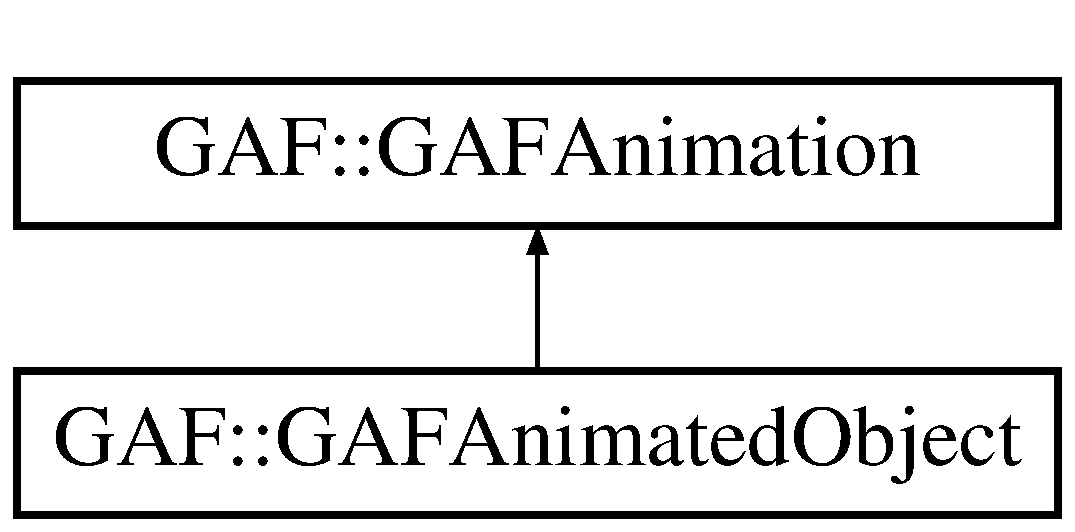
\includegraphics[height=2.000000cm]{class_g_a_f_1_1_g_a_f_animation}
\end{center}
\end{figure}
\subsection*{Public Member Functions}
\begin{DoxyCompactItemize}
\item 
\hypertarget{class_g_a_f_1_1_g_a_f_animation_ad410402f6fad09729559a1abd7d48a9c}{bool {\bfseries init} (\hyperlink{class_g_a_f_1_1_g_a_f_asset}{G\-A\-F\-Asset} $\ast$an\-Animation\-Data)}\label{class_g_a_f_1_1_g_a_f_animation_ad410402f6fad09729559a1abd7d48a9c}

\item 
\hypertarget{class_g_a_f_1_1_g_a_f_animation_a62cc9254f7ebf0a7f47ae21536bebc3a}{virtual void {\bfseries process\-Animation} ()}\label{class_g_a_f_1_1_g_a_f_animation_a62cc9254f7ebf0a7f47ae21536bebc3a}

\item 
\hypertarget{class_g_a_f_1_1_g_a_f_animation_a4a80038816578473a98184d7f5441240}{virtual void {\bfseries start} ()}\label{class_g_a_f_1_1_g_a_f_animation_a4a80038816578473a98184d7f5441240}

\item 
\hypertarget{class_g_a_f_1_1_g_a_f_animation_a2f7f1038c4964b50398bdb3bcb209fda}{virtual void {\bfseries pause} ()}\label{class_g_a_f_1_1_g_a_f_animation_a2f7f1038c4964b50398bdb3bcb209fda}

\item 
\hypertarget{class_g_a_f_1_1_g_a_f_animation_a7269d57c04597b93790c5835e6d76fee}{virtual void {\bfseries resume} ()}\label{class_g_a_f_1_1_g_a_f_animation_a7269d57c04597b93790c5835e6d76fee}

\item 
\hypertarget{class_g_a_f_1_1_g_a_f_animation_a5651703f8d875d4cd64d966cd8ff1464}{virtual void \hyperlink{class_g_a_f_1_1_g_a_f_animation_a5651703f8d875d4cd64d966cd8ff1464}{stop} ()}\label{class_g_a_f_1_1_g_a_f_animation_a5651703f8d875d4cd64d966cd8ff1464}

\begin{DoxyCompactList}\small\item\em Stops animation and sets the current\-Frame pointer to the first frame. \end{DoxyCompactList}\item 
\hypertarget{class_g_a_f_1_1_g_a_f_animation_aebc7d8df72a869a5b05d4746f6cd0a90}{virtual void {\bfseries step} ()}\label{class_g_a_f_1_1_g_a_f_animation_aebc7d8df72a869a5b05d4746f6cd0a90}

\item 
bool \hyperlink{class_g_a_f_1_1_g_a_f_animation_a64a17e6305d1ada5f37d2636ce098816}{is\-Done} () const 
\item 
\hypertarget{class_g_a_f_1_1_g_a_f_animation_a456363aeb317e9259e3442cde27b103c}{bool {\bfseries is\-Animation\-Running} () const }\label{class_g_a_f_1_1_g_a_f_animation_a456363aeb317e9259e3442cde27b103c}

\item 
\hypertarget{class_g_a_f_1_1_g_a_f_animation_ab092a453363a99bedd33afb2bdebf963}{bool {\bfseries is\-Looped} () const }\label{class_g_a_f_1_1_g_a_f_animation_ab092a453363a99bedd33afb2bdebf963}

\item 
\hypertarget{class_g_a_f_1_1_g_a_f_animation_ab2580732c42e2511dbd7e9cdfa90cd5d}{void {\bfseries set\-Looped} (bool looped)}\label{class_g_a_f_1_1_g_a_f_animation_ab2580732c42e2511dbd7e9cdfa90cd5d}

\item 
\hypertarget{class_g_a_f_1_1_g_a_f_animation_a821d3864f9d3f903747050b5a86c6bbb}{int {\bfseries total\-Frame\-Count} () const }\label{class_g_a_f_1_1_g_a_f_animation_a821d3864f9d3f903747050b5a86c6bbb}

\item 
\hypertarget{class_g_a_f_1_1_g_a_f_animation_a082c85367b5c28f56a71308bcd6f0a62}{int {\bfseries current\-Frame\-Index} () const }\label{class_g_a_f_1_1_g_a_f_animation_a082c85367b5c28f56a71308bcd6f0a62}

\item 
\hypertarget{class_g_a_f_1_1_g_a_f_animation_ac296331cff3413e04cada85ca611c8e5}{bool {\bfseries set\-Frame} (int index)}\label{class_g_a_f_1_1_g_a_f_animation_ac296331cff3413e04cada85ca611c8e5}

\item 
\hypertarget{class_g_a_f_1_1_g_a_f_animation_a6f788433e2c18fd8e932480346b03f58}{bool {\bfseries goto\-And\-Stop} (const char $\ast$frame\-Label)}\label{class_g_a_f_1_1_g_a_f_animation_a6f788433e2c18fd8e932480346b03f58}

\item 
\hypertarget{class_g_a_f_1_1_g_a_f_animation_ad8a413735c23f93b2d6914454244802d}{bool \hyperlink{class_g_a_f_1_1_g_a_f_animation_ad8a413735c23f93b2d6914454244802d}{goto\-And\-Stop} (int frame\-Number)}\label{class_g_a_f_1_1_g_a_f_animation_ad8a413735c23f93b2d6914454244802d}

\begin{DoxyCompactList}\small\item\em Plays specified frame and then stops. \end{DoxyCompactList}\item 
\hypertarget{class_g_a_f_1_1_g_a_f_animation_a67a0740196dc67a9c8358bca8290d9ea}{bool {\bfseries goto\-And\-Play} (const char $\ast$frame\-Label)}\label{class_g_a_f_1_1_g_a_f_animation_a67a0740196dc67a9c8358bca8290d9ea}

\item 
\hypertarget{class_g_a_f_1_1_g_a_f_animation_a47b7d4bf50567a802c9dd7c9db9c4f2e}{bool \hyperlink{class_g_a_f_1_1_g_a_f_animation_a47b7d4bf50567a802c9dd7c9db9c4f2e}{goto\-And\-Play} (int frame\-Number)}\label{class_g_a_f_1_1_g_a_f_animation_a47b7d4bf50567a802c9dd7c9db9c4f2e}

\begin{DoxyCompactList}\small\item\em Plays animation from specified frame. \end{DoxyCompactList}\item 
\hypertarget{class_g_a_f_1_1_g_a_f_animation_ac89a67e10a2d924e61fad7abd8425941}{int {\bfseries get\-Start\-Frame} (const char $\ast$frame\-Label)}\label{class_g_a_f_1_1_g_a_f_animation_ac89a67e10a2d924e61fad7abd8425941}

\item 
\hypertarget{class_g_a_f_1_1_g_a_f_animation_acba2cb2c2419810c4844dd2ae9f8e3d7}{int {\bfseries get\-End\-Frame} (const char $\ast$frame\-Label)}\label{class_g_a_f_1_1_g_a_f_animation_acba2cb2c2419810c4844dd2ae9f8e3d7}

\item 
bool \hyperlink{class_g_a_f_1_1_g_a_f_animation_ad028c73c5230df3d28c17a64308affc6}{play\-Sequence} (const char $\ast$name, bool looped=false, bool resume=true, Anim\-Set\-Sequence\-Hint hint=A\-S\-S\-H\-\_\-\-R\-E\-S\-T\-A\-R\-T)
\item 
\hypertarget{class_g_a_f_1_1_g_a_f_animation_a5e511bc4a57e19db743aab01b66fc479}{void {\bfseries clear\-Sequence} ()}\label{class_g_a_f_1_1_g_a_f_animation_a5e511bc4a57e19db743aab01b66fc479}

\item 
void \hyperlink{class_g_a_f_1_1_g_a_f_animation_a2cb44dad0426d774ee28597b5d09dca5}{set\-Sequence\-Delegate} (\hyperlink{class_g_a_f_1_1_g_a_f_sequence_delegate}{G\-A\-F\-Sequence\-Delegate} $\ast$delegate)
\end{DoxyCompactItemize}
\subsection*{Protected Attributes}
\begin{DoxyCompactItemize}
\item 
\hypertarget{class_g_a_f_1_1_g_a_f_animation_a5237206b9ce62ef7cf8701f6c8a529da}{\hyperlink{class_g_a_f_1_1_g_a_f_asset}{G\-A\-F\-Asset} $\ast$ {\bfseries \-\_\-asset}}\label{class_g_a_f_1_1_g_a_f_animation_a5237206b9ce62ef7cf8701f6c8a529da}

\item 
\hypertarget{class_g_a_f_1_1_g_a_f_animation_a05555677b7af6a0c1b5e6bed2c4aeed0}{int {\bfseries \-\_\-current\-Frame\-Index}}\label{class_g_a_f_1_1_g_a_f_animation_a05555677b7af6a0c1b5e6bed2c4aeed0}

\end{DoxyCompactItemize}


\subsection{Member Function Documentation}
\hypertarget{class_g_a_f_1_1_g_a_f_animation_a64a17e6305d1ada5f37d2636ce098816}{\index{G\-A\-F\-::\-G\-A\-F\-Animation@{G\-A\-F\-::\-G\-A\-F\-Animation}!is\-Done@{is\-Done}}
\index{is\-Done@{is\-Done}!GAF::GAFAnimation@{G\-A\-F\-::\-G\-A\-F\-Animation}}
\subsubsection[{is\-Done}]{\setlength{\rightskip}{0pt plus 5cm}bool G\-A\-F\-::\-G\-A\-F\-Animation\-::is\-Done (
\begin{DoxyParamCaption}
{}
\end{DoxyParamCaption}
) const}}\label{class_g_a_f_1_1_g_a_f_animation_a64a17e6305d1ada5f37d2636ce098816}
\begin{DoxyReturn}{Returns}
true if the animation is finished, otherwise N\-O 
\end{DoxyReturn}
\hypertarget{class_g_a_f_1_1_g_a_f_animation_ad028c73c5230df3d28c17a64308affc6}{\index{G\-A\-F\-::\-G\-A\-F\-Animation@{G\-A\-F\-::\-G\-A\-F\-Animation}!play\-Sequence@{play\-Sequence}}
\index{play\-Sequence@{play\-Sequence}!GAF::GAFAnimation@{G\-A\-F\-::\-G\-A\-F\-Animation}}
\subsubsection[{play\-Sequence}]{\setlength{\rightskip}{0pt plus 5cm}bool G\-A\-F\-::\-G\-A\-F\-Animation\-::play\-Sequence (
\begin{DoxyParamCaption}
\item[{const char $\ast$}]{name, }
\item[{bool}]{looped = {\ttfamily false}, }
\item[{bool}]{resume = {\ttfamily true}, }
\item[{Anim\-Set\-Sequence\-Hint}]{hint = {\ttfamily ASSH\-\_\-RESTART}}
\end{DoxyParamCaption}
)}}\label{class_g_a_f_1_1_g_a_f_animation_ad028c73c5230df3d28c17a64308affc6}
Plays animation sequence with specified name 
\begin{DoxyParams}{Parameters}
{\em name} & a sequence name \\
\hline
{\em looped} & if true -\/ sequence should play in cycle \\
\hline
{\em resume} & if true -\/ animation will be played immediately, if false -\/ playback will be paused after the first frame is shown \\
\hline
{\em hint} & specific animation playback parameters \\
\hline
\end{DoxyParams}
\hypertarget{class_g_a_f_1_1_g_a_f_animation_a2cb44dad0426d774ee28597b5d09dca5}{\index{G\-A\-F\-::\-G\-A\-F\-Animation@{G\-A\-F\-::\-G\-A\-F\-Animation}!set\-Sequence\-Delegate@{set\-Sequence\-Delegate}}
\index{set\-Sequence\-Delegate@{set\-Sequence\-Delegate}!GAF::GAFAnimation@{G\-A\-F\-::\-G\-A\-F\-Animation}}
\subsubsection[{set\-Sequence\-Delegate}]{\setlength{\rightskip}{0pt plus 5cm}void G\-A\-F\-::\-G\-A\-F\-Animation\-::set\-Sequence\-Delegate (
\begin{DoxyParamCaption}
\item[{{\bf G\-A\-F\-Sequence\-Delegate} $\ast$}]{delegate}
\end{DoxyParamCaption}
)}}\label{class_g_a_f_1_1_g_a_f_animation_a2cb44dad0426d774ee28597b5d09dca5}
\begin{DoxyNote}{Note}
do not forget to call set\-Sequence\-Delegate(\-N\-U\-L\-L) before deleting your subscriber 
\end{DoxyNote}


The documentation for this class was generated from the following file\-:\begin{DoxyCompactItemize}
\item 
G\-A\-F\-Animation.\-h\end{DoxyCompactItemize}

\hypertarget{class_g_a_f_1_1_g_a_f_animation_frame}{\section{G\-A\-F\-:\-:G\-A\-F\-Animation\-Frame Class Reference}
\label{class_g_a_f_1_1_g_a_f_animation_frame}\index{G\-A\-F\-::\-G\-A\-F\-Animation\-Frame@{G\-A\-F\-::\-G\-A\-F\-Animation\-Frame}}
}
Inheritance diagram for G\-A\-F\-:\-:G\-A\-F\-Animation\-Frame\-:\begin{figure}[H]
\begin{center}
\leavevmode
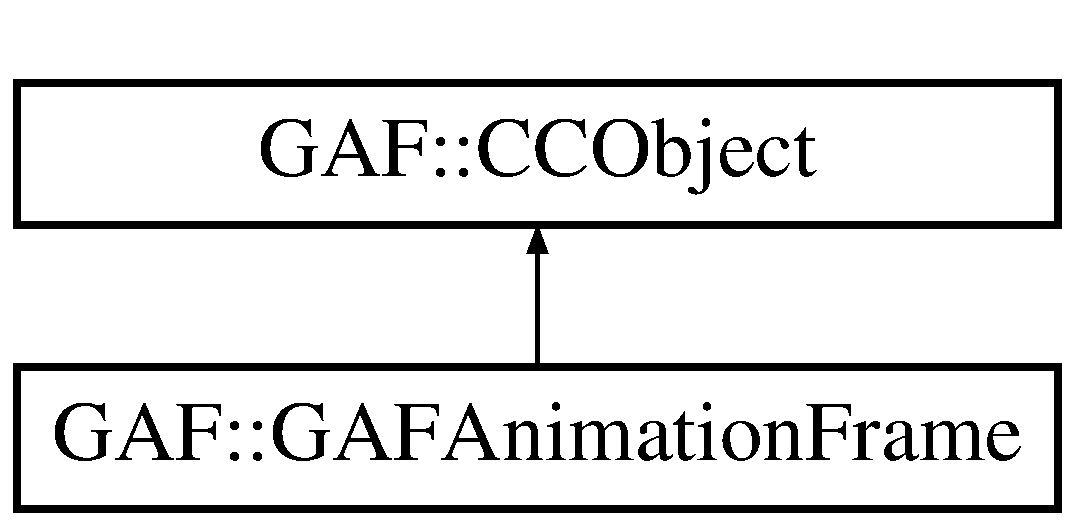
\includegraphics[height=2.000000cm]{class_g_a_f_1_1_g_a_f_animation_frame}
\end{center}
\end{figure}
\subsection*{Public Member Functions}
\begin{DoxyCompactItemize}
\item 
\hypertarget{class_g_a_f_1_1_g_a_f_animation_frame_aaab8e694d9f2c0e76490f365e2364244}{\hyperlink{class_g_a_f_1_1_c_c_array}{C\-C\-Array} $\ast$ {\bfseries object\-States} ()}\label{class_g_a_f_1_1_g_a_f_animation_frame_aaab8e694d9f2c0e76490f365e2364244}

\item 
\hypertarget{class_g_a_f_1_1_g_a_f_animation_frame_ae2124eb7022d6f60d09600cb8b7c2570}{void {\bfseries set\-Object\-States} (\hyperlink{class_g_a_f_1_1_c_c_array}{C\-C\-Array} $\ast$states)}\label{class_g_a_f_1_1_g_a_f_animation_frame_ae2124eb7022d6f60d09600cb8b7c2570}

\end{DoxyCompactItemize}


The documentation for this class was generated from the following file\-:\begin{DoxyCompactItemize}
\item 
G\-A\-F\-Animation\-Frame.\-h\end{DoxyCompactItemize}

\hypertarget{class_g_a_f_1_1_g_a_f_animation_sequence}{\section{G\-A\-F\-:\-:G\-A\-F\-Animation\-Sequence Class Reference}
\label{class_g_a_f_1_1_g_a_f_animation_sequence}\index{G\-A\-F\-::\-G\-A\-F\-Animation\-Sequence@{G\-A\-F\-::\-G\-A\-F\-Animation\-Sequence}}
}
Inheritance diagram for G\-A\-F\-:\-:G\-A\-F\-Animation\-Sequence\-:\begin{figure}[H]
\begin{center}
\leavevmode
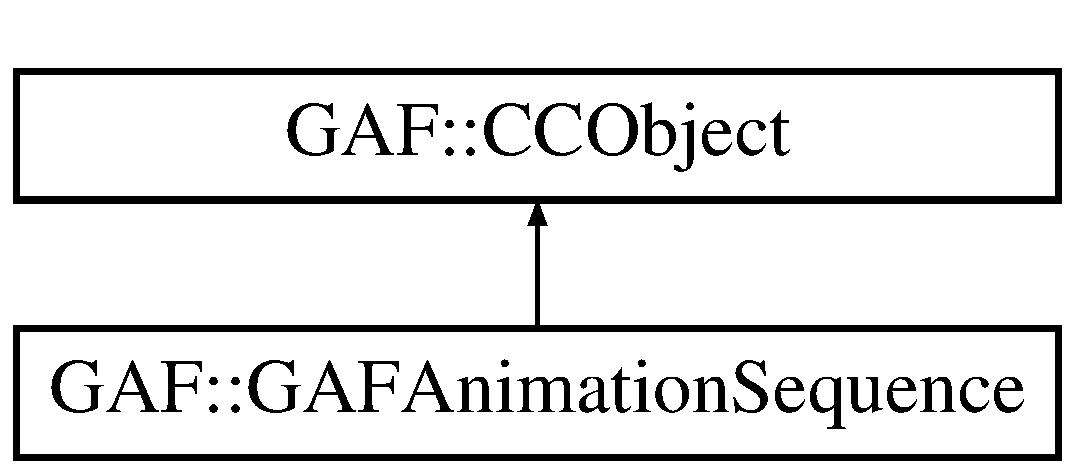
\includegraphics[height=2.000000cm]{class_g_a_f_1_1_g_a_f_animation_sequence}
\end{center}
\end{figure}
\subsection*{Public Member Functions}
\begin{DoxyCompactItemize}
\item 
\hypertarget{class_g_a_f_1_1_g_a_f_animation_sequence_a9cde0aeefe0013f12746f424139ed5be}{int {\bfseries length} () const }\label{class_g_a_f_1_1_g_a_f_animation_sequence_a9cde0aeefe0013f12746f424139ed5be}

\end{DoxyCompactItemize}
\subsection*{Public Attributes}
\begin{DoxyCompactItemize}
\item 
\hypertarget{class_g_a_f_1_1_g_a_f_animation_sequence_a7589a1bf527f6ff96c41b5722af7d9ab}{std\-::string {\bfseries name}}\label{class_g_a_f_1_1_g_a_f_animation_sequence_a7589a1bf527f6ff96c41b5722af7d9ab}

\item 
\hypertarget{class_g_a_f_1_1_g_a_f_animation_sequence_a5cd0c1aeb0565a2b839dedbd5a603a50}{int {\bfseries start\-Frame\-No}}\label{class_g_a_f_1_1_g_a_f_animation_sequence_a5cd0c1aeb0565a2b839dedbd5a603a50}

\item 
\hypertarget{class_g_a_f_1_1_g_a_f_animation_sequence_a936b4cf7ba81d69ab2e6c798558d434e}{int {\bfseries end\-Frame\-No}}\label{class_g_a_f_1_1_g_a_f_animation_sequence_a936b4cf7ba81d69ab2e6c798558d434e}

\end{DoxyCompactItemize}


The documentation for this class was generated from the following file\-:\begin{DoxyCompactItemize}
\item 
G\-A\-F\-Animation\-Sequence.\-h\end{DoxyCompactItemize}

\hypertarget{class_g_a_f_1_1_g_a_f_asset}{\section{G\-A\-F\-:\-:G\-A\-F\-Asset Class Reference}
\label{class_g_a_f_1_1_g_a_f_asset}\index{G\-A\-F\-::\-G\-A\-F\-Asset@{G\-A\-F\-::\-G\-A\-F\-Asset}}
}
Inheritance diagram for G\-A\-F\-:\-:G\-A\-F\-Asset\-:\begin{figure}[H]
\begin{center}
\leavevmode
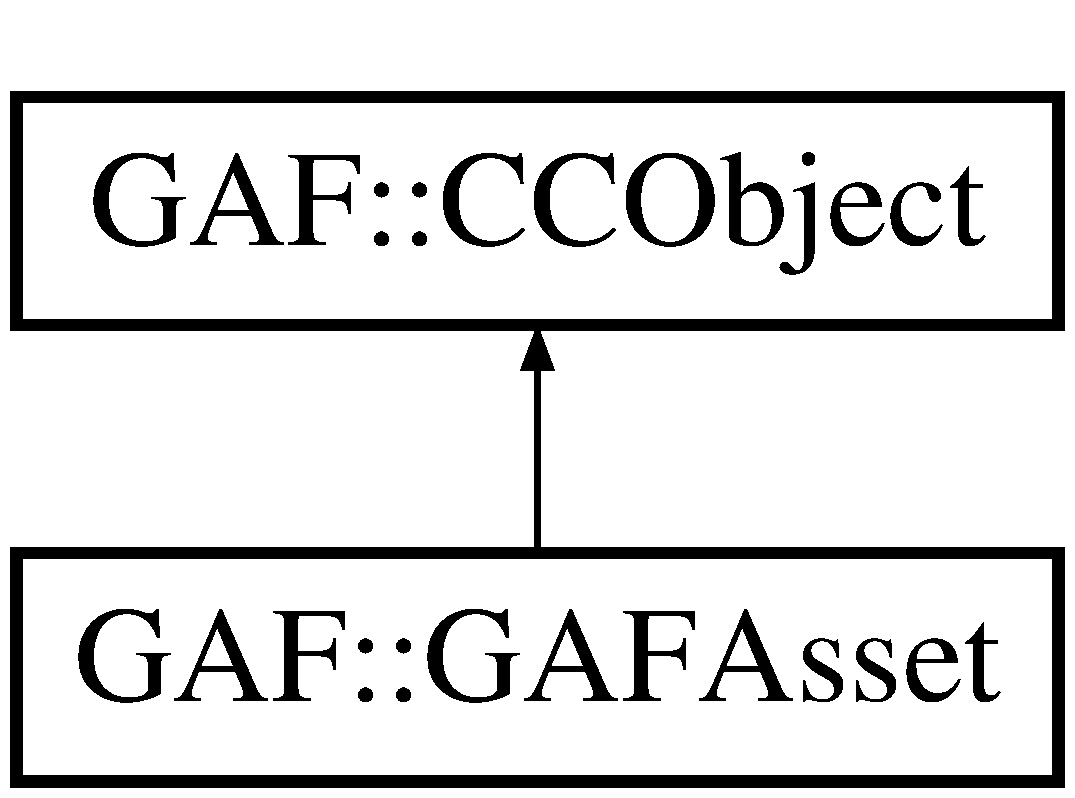
\includegraphics[height=2.000000cm]{class_g_a_f_1_1_g_a_f_asset}
\end{center}
\end{figure}
\subsection*{Public Member Functions}
\begin{DoxyCompactItemize}
\item 
\hypertarget{class_g_a_f_1_1_g_a_f_asset_a4f0ec3dad0ad82b5c7963a7ac26c7372}{bool {\bfseries init\-With\-Image\-Data} (const std\-::string \&json\-Path)}\label{class_g_a_f_1_1_g_a_f_asset_a4f0ec3dad0ad82b5c7963a7ac26c7372}

\item 
\hypertarget{class_g_a_f_1_1_g_a_f_asset_ac8b3c99a8a082a02d32168a6e6720da2}{int \hyperlink{class_g_a_f_1_1_g_a_f_asset_ac8b3c99a8a082a02d32168a6e6720da2}{animation\-Frames\-Count} () const }\label{class_g_a_f_1_1_g_a_f_asset_ac8b3c99a8a082a02d32168a6e6720da2}

\begin{DoxyCompactList}\small\item\em total number of frames in animation \end{DoxyCompactList}\item 
\hypertarget{class_g_a_f_1_1_g_a_f_asset_a9fced4b3b2f2060fcd5a18ef4d584fc6}{\hyperlink{class_g_a_f_1_1_g_a_f_texture_atlas}{G\-A\-F\-Texture\-Atlas} $\ast$ {\bfseries texture\-Atlas} ()}\label{class_g_a_f_1_1_g_a_f_asset_a9fced4b3b2f2060fcd5a18ef4d584fc6}

\item 
\hypertarget{class_g_a_f_1_1_g_a_f_asset_a7313ebc47dc135db64e11ff8d78f100e}{\hyperlink{class_g_a_f_1_1_c_c_dictionary}{C\-C\-Dictionary} $\ast$ \hyperlink{class_g_a_f_1_1_g_a_f_asset_a7313ebc47dc135db64e11ff8d78f100e}{objects} ()}\label{class_g_a_f_1_1_g_a_f_asset_a7313ebc47dc135db64e11ff8d78f100e}

\begin{DoxyCompactList}\small\item\em Dictionary of objects \mbox{[}Object\-Id -\/$>$ Atlas\-Element\-Name\mbox{]}. \end{DoxyCompactList}\item 
\hypertarget{class_g_a_f_1_1_g_a_f_asset_a1b82f9cf2556eeb8f642d1f2317d66af}{\hyperlink{class_g_a_f_1_1_c_c_dictionary}{C\-C\-Dictionary} $\ast$ \hyperlink{class_g_a_f_1_1_g_a_f_asset_a1b82f9cf2556eeb8f642d1f2317d66af}{masks} ()}\label{class_g_a_f_1_1_g_a_f_asset_a1b82f9cf2556eeb8f642d1f2317d66af}

\begin{DoxyCompactList}\small\item\em Dictionary of masks \mbox{[}Mask\-Id -\/$>$ Atlas\-Element\-Name\mbox{]}. \end{DoxyCompactList}\item 
\hypertarget{class_g_a_f_1_1_g_a_f_asset_a7e9ebad7448f699ef459227093086fe2}{\hyperlink{class_g_a_f_1_1_c_c_dictionary}{C\-C\-Dictionary} $\ast$ \hyperlink{class_g_a_f_1_1_g_a_f_asset_a7e9ebad7448f699ef459227093086fe2}{named\-Parts} ()}\label{class_g_a_f_1_1_g_a_f_asset_a7e9ebad7448f699ef459227093086fe2}

\begin{DoxyCompactList}\small\item\em Dictionary of masks \mbox{[}Mask\-Id -\/$>$ Atlas\-Element\-Name\mbox{]}. \end{DoxyCompactList}\item 
\hypertarget{class_g_a_f_1_1_g_a_f_asset_acd15bfc31ea707bd08e6080fea76ef3e}{\hyperlink{class_g_a_f_1_1_c_c_dictionary}{C\-C\-Dictionary} $\ast$ \hyperlink{class_g_a_f_1_1_g_a_f_asset_acd15bfc31ea707bd08e6080fea76ef3e}{animation\-Sequences} ()}\label{class_g_a_f_1_1_g_a_f_asset_acd15bfc31ea707bd08e6080fea76ef3e}

\begin{DoxyCompactList}\small\item\em List of G\-A\-F\-Animation\-Sequences objects. \end{DoxyCompactList}\item 
\hypertarget{class_g_a_f_1_1_g_a_f_asset_ab28aad7bb6081207de2e6f0871c64757}{\hyperlink{class_g_a_f_1_1_g_a_f_animation_sequence}{G\-A\-F\-Animation\-Sequence} $\ast$ \hyperlink{class_g_a_f_1_1_g_a_f_asset_ab28aad7bb6081207de2e6f0871c64757}{get\-Sequence} (const char $\ast$name)}\label{class_g_a_f_1_1_g_a_f_asset_ab28aad7bb6081207de2e6f0871c64757}

\begin{DoxyCompactList}\small\item\em get \hyperlink{class_g_a_f_1_1_g_a_f_animation_sequence}{G\-A\-F\-Animation\-Sequence} by name specified in editor \end{DoxyCompactList}\item 
\hypertarget{class_g_a_f_1_1_g_a_f_asset_a31432e877bd659fbfd1fde8b99251562}{\hyperlink{class_g_a_f_1_1_g_a_f_animation_sequence}{G\-A\-F\-Animation\-Sequence} $\ast$ \hyperlink{class_g_a_f_1_1_g_a_f_asset_a31432e877bd659fbfd1fde8b99251562}{get\-Sequence\-By\-Last\-Frame} (int frame)}\label{class_g_a_f_1_1_g_a_f_asset_a31432e877bd659fbfd1fde8b99251562}

\begin{DoxyCompactList}\small\item\em get \hyperlink{class_g_a_f_1_1_g_a_f_animation_sequence}{G\-A\-F\-Animation\-Sequence} by last frame number in sequence \end{DoxyCompactList}\item 
\hypertarget{class_g_a_f_1_1_g_a_f_asset_a9fee929a803e67ad2cb50b5de16c315a}{\hyperlink{class_g_a_f_1_1_c_c_array}{C\-C\-Array} $\ast$ \hyperlink{class_g_a_f_1_1_g_a_f_asset_a9fee929a803e67ad2cb50b5de16c315a}{animation\-Frames} ()}\label{class_g_a_f_1_1_g_a_f_asset_a9fee929a803e67ad2cb50b5de16c315a}

\begin{DoxyCompactList}\small\item\em List of \hyperlink{class_g_a_f_1_1_g_a_f_animation_frame}{G\-A\-F\-Animation\-Frame} objects. \end{DoxyCompactList}\item 
\hypertarget{class_g_a_f_1_1_g_a_f_asset_a675440c329d07af3dd70e52316ddaea5}{\hyperlink{class_g_a_f_1_1_g_a_f_animated_object}{G\-A\-F\-Animated\-Object} $\ast$ {\bfseries create\-Object} ()}\label{class_g_a_f_1_1_g_a_f_asset_a675440c329d07af3dd70e52316ddaea5}

\item 
\hypertarget{class_g_a_f_1_1_g_a_f_asset_a1b8286f43e4d5bb4f6b19d5d97965098}{\hyperlink{class_g_a_f_1_1_g_a_f_animated_object}{G\-A\-F\-Animated\-Object} $\ast$ {\bfseries create\-Object\-And\-Run} (bool looped=false)}\label{class_g_a_f_1_1_g_a_f_asset_a1b8286f43e4d5bb4f6b19d5d97965098}

\item 
\hypertarget{class_g_a_f_1_1_g_a_f_asset_a1016caada738c542caaea76baa415439}{float \hyperlink{class_g_a_f_1_1_g_a_f_asset_a1016caada738c542caaea76baa415439}{used\-Atlas\-Csf} () const }\label{class_g_a_f_1_1_g_a_f_asset_a1016caada738c542caaea76baa415439}

\begin{DoxyCompactList}\small\item\em used content scale factor \end{DoxyCompactList}\end{DoxyCompactItemize}
\subsection*{Static Public Member Functions}
\begin{DoxyCompactItemize}
\item 
\hypertarget{class_g_a_f_1_1_g_a_f_asset_a339f17f57d9f1ee0aaf937bc04f68484}{static \hyperlink{class_g_a_f_1_1_g_a_f_asset}{G\-A\-F\-Asset} $\ast$ \hyperlink{class_g_a_f_1_1_g_a_f_asset_a339f17f57d9f1ee0aaf937bc04f68484}{create} (const std\-::string \&json\-Path)}\label{class_g_a_f_1_1_g_a_f_asset_a339f17f57d9f1ee0aaf937bc04f68484}

\begin{DoxyCompactList}\small\item\em Initializes asset with J\-S\-O\-N data. \end{DoxyCompactList}\item 
\hypertarget{class_g_a_f_1_1_g_a_f_asset_a003a54790c5f383bf72b2918ec14335f}{static bool {\bfseries is\-Asset\-Version\-Playable} (const char $\ast$version)}\label{class_g_a_f_1_1_g_a_f_asset_a003a54790c5f383bf72b2918ec14335f}

\item 
\hypertarget{class_g_a_f_1_1_g_a_f_asset_a76d2a115303d19e6543a009bd75e280e}{static int \hyperlink{class_g_a_f_1_1_g_a_f_asset_a76d2a115303d19e6543a009bd75e280e}{desired\-Csf} ()}\label{class_g_a_f_1_1_g_a_f_asset_a76d2a115303d19e6543a009bd75e280e}

\begin{DoxyCompactList}\small\item\em desired content scale factor \end{DoxyCompactList}\item 
\hypertarget{class_g_a_f_1_1_g_a_f_asset_afa4fb372779763d31793bdf73cf22dd8}{static void \hyperlink{class_g_a_f_1_1_g_a_f_asset_afa4fb372779763d31793bdf73cf22dd8}{set\-Desired\-Csf} (int csf)}\label{class_g_a_f_1_1_g_a_f_asset_afa4fb372779763d31793bdf73cf22dd8}

\begin{DoxyCompactList}\small\item\em sets desired content scale factor \end{DoxyCompactList}\end{DoxyCompactItemize}


The documentation for this class was generated from the following file\-:\begin{DoxyCompactItemize}
\item 
G\-A\-F\-Asset.\-h\end{DoxyCompactItemize}

\hypertarget{class_g_a_f_1_1_g_a_f_blur_filter_data}{\section{G\-A\-F\-:\-:G\-A\-F\-Blur\-Filter\-Data Class Reference}
\label{class_g_a_f_1_1_g_a_f_blur_filter_data}\index{G\-A\-F\-::\-G\-A\-F\-Blur\-Filter\-Data@{G\-A\-F\-::\-G\-A\-F\-Blur\-Filter\-Data}}
}
Inheritance diagram for G\-A\-F\-:\-:G\-A\-F\-Blur\-Filter\-Data\-:\begin{figure}[H]
\begin{center}
\leavevmode
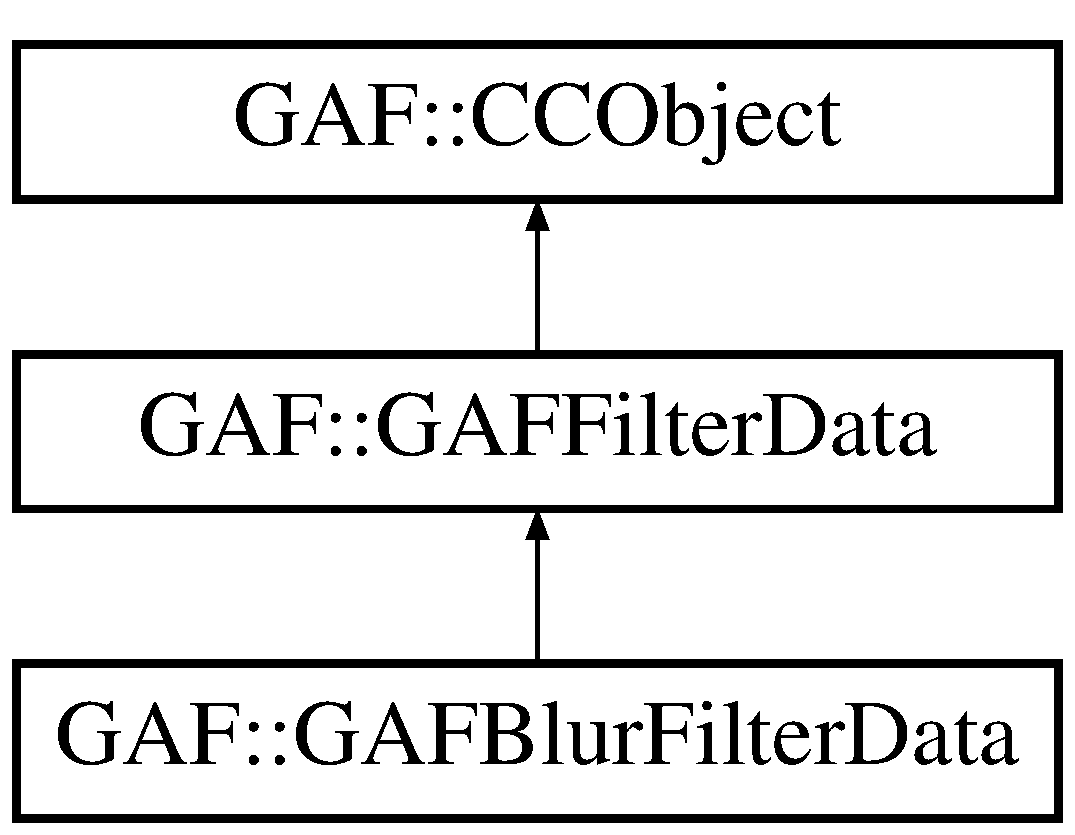
\includegraphics[height=3.000000cm]{class_g_a_f_1_1_g_a_f_blur_filter_data}
\end{center}
\end{figure}
\subsection*{Static Public Member Functions}
\begin{DoxyCompactItemize}
\item 
\hypertarget{class_g_a_f_1_1_g_a_f_blur_filter_data_a2959c14e886df2e3d00bacfa513b7f74}{static \hyperlink{class_g_a_f_1_1_g_a_f_blur_filter_data}{G\-A\-F\-Blur\-Filter\-Data} $\ast$ {\bfseries create} (float \-\_\-blur\-X, float \-\_\-blur\-Y)}\label{class_g_a_f_1_1_g_a_f_blur_filter_data_a2959c14e886df2e3d00bacfa513b7f74}

\end{DoxyCompactItemize}
\subsection*{Public Attributes}
\begin{DoxyCompactItemize}
\item 
\hypertarget{class_g_a_f_1_1_g_a_f_blur_filter_data_a3b3250afccae332781a2942c22981ff2}{\hyperlink{class_g_a_f_1_1_c_c_size}{C\-C\-Size} {\bfseries blur\-Size}}\label{class_g_a_f_1_1_g_a_f_blur_filter_data_a3b3250afccae332781a2942c22981ff2}

\end{DoxyCompactItemize}
\subsection*{Additional Inherited Members}


The documentation for this class was generated from the following file\-:\begin{DoxyCompactItemize}
\item 
G\-A\-F\-Filter\-Data.\-h\end{DoxyCompactItemize}

\hypertarget{class_g_a_f_1_1_g_a_f_data}{\section{G\-A\-F\-:\-:G\-A\-F\-Data Class Reference}
\label{class_g_a_f_1_1_g_a_f_data}\index{G\-A\-F\-::\-G\-A\-F\-Data@{G\-A\-F\-::\-G\-A\-F\-Data}}
}


{\ttfamily \#include $<$G\-A\-F\-Data.\-h$>$}

Inheritance diagram for G\-A\-F\-:\-:G\-A\-F\-Data\-:\begin{figure}[H]
\begin{center}
\leavevmode
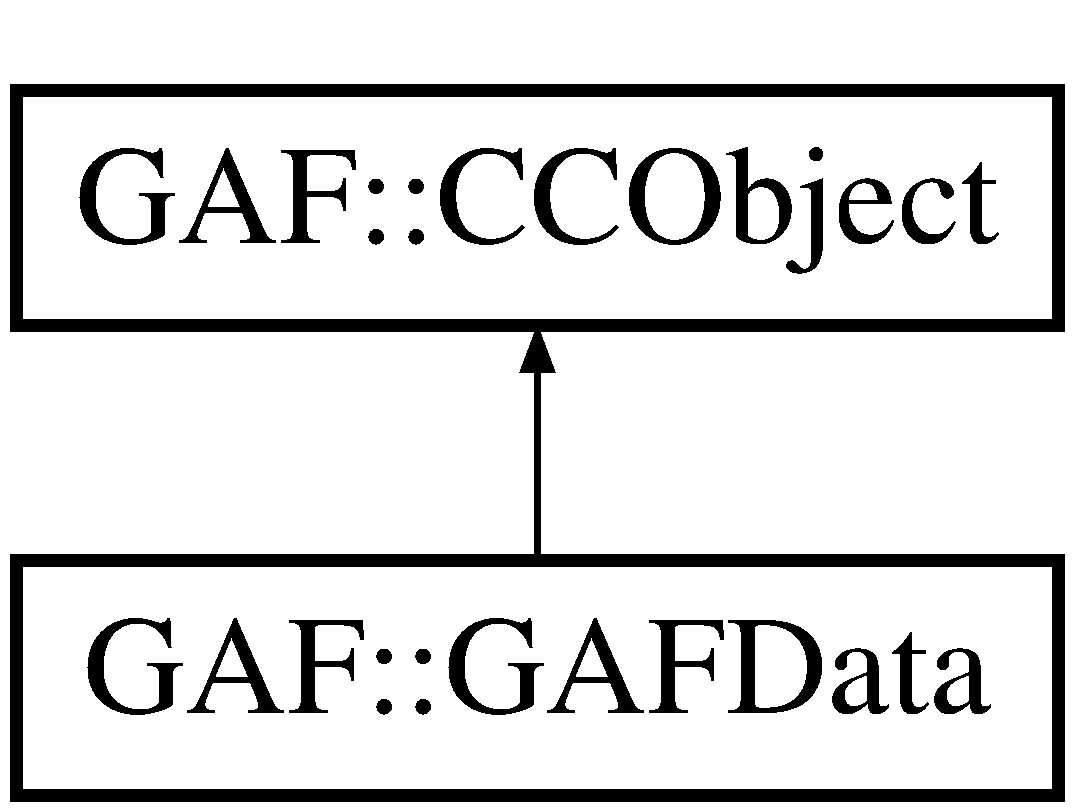
\includegraphics[height=2.000000cm]{class_g_a_f_1_1_g_a_f_data}
\end{center}
\end{figure}
\subsection*{Public Member Functions}
\begin{DoxyCompactItemize}
\item 
\hypertarget{class_g_a_f_1_1_g_a_f_data_aef1f44d75c6f72f2d28e24c7a3fd1a1f}{{\bfseries G\-A\-F\-Data} (unsigned char $\ast$\-\_\-ptr, int size, bool delete\-\_\-data=false)}\label{class_g_a_f_1_1_g_a_f_data_aef1f44d75c6f72f2d28e24c7a3fd1a1f}

\item 
\hypertarget{class_g_a_f_1_1_g_a_f_data_a20ce92e7efd7fb55b57e373b747515d1}{unsigned char $\ast$ {\bfseries bytes} () const }\label{class_g_a_f_1_1_g_a_f_data_a20ce92e7efd7fb55b57e373b747515d1}

\item 
\hypertarget{class_g_a_f_1_1_g_a_f_data_a9ddeff084b3c488fadec36afeaf24354}{void {\bfseries set\-Bytes} (unsigned char $\ast$bytes)}\label{class_g_a_f_1_1_g_a_f_data_a9ddeff084b3c488fadec36afeaf24354}

\item 
\hypertarget{class_g_a_f_1_1_g_a_f_data_aaabf7529ff1314ed6bbe0381c3dd2d9f}{unsigned long {\bfseries size} () const }\label{class_g_a_f_1_1_g_a_f_data_aaabf7529ff1314ed6bbe0381c3dd2d9f}

\item 
\hypertarget{class_g_a_f_1_1_g_a_f_data_a32f7e574f4f2afbb76dd0f07594e64e9}{void {\bfseries set\-Size} (unsigned long size)}\label{class_g_a_f_1_1_g_a_f_data_a32f7e574f4f2afbb76dd0f07594e64e9}

\item 
void \hyperlink{class_g_a_f_1_1_g_a_f_data_a562c8e9f3b3ba2713c16286a4e6bcf41}{set\-Delete\-Data} (bool delete\-Data)
\end{DoxyCompactItemize}


\subsection{Detailed Description}
Simple N\-S\-Data-\/like class for internal usage. Made public since it can be useful for G\-A\-F Marmalade users. It does N\-O\-T release memory by default -\/ be careful. 

\subsection{Member Function Documentation}
\hypertarget{class_g_a_f_1_1_g_a_f_data_a562c8e9f3b3ba2713c16286a4e6bcf41}{\index{G\-A\-F\-::\-G\-A\-F\-Data@{G\-A\-F\-::\-G\-A\-F\-Data}!set\-Delete\-Data@{set\-Delete\-Data}}
\index{set\-Delete\-Data@{set\-Delete\-Data}!GAF::GAFData@{G\-A\-F\-::\-G\-A\-F\-Data}}
\subsubsection[{set\-Delete\-Data}]{\setlength{\rightskip}{0pt plus 5cm}void G\-A\-F\-::\-G\-A\-F\-Data\-::set\-Delete\-Data (
\begin{DoxyParamCaption}
\item[{bool}]{delete\-Data}
\end{DoxyParamCaption}
)\hspace{0.3cm}{\ttfamily [inline]}}}\label{class_g_a_f_1_1_g_a_f_data_a562c8e9f3b3ba2713c16286a4e6bcf41}
By default \hyperlink{class_g_a_f_1_1_g_a_f_data}{G\-A\-F\-Data} does N\-O\-T release memory. However, it is possible to delete internal array in destructor. 
\begin{DoxyParams}{Parameters}
{\em delete\-Data} & -\/ delete internal array in desctructor or not \\
\hline
\end{DoxyParams}


The documentation for this class was generated from the following file\-:\begin{DoxyCompactItemize}
\item 
G\-A\-F\-Data.\-h\end{DoxyCompactItemize}

\hypertarget{class_g_a_f_1_1_g_a_f_filter_data}{\section{G\-A\-F\-:\-:G\-A\-F\-Filter\-Data Class Reference}
\label{class_g_a_f_1_1_g_a_f_filter_data}\index{G\-A\-F\-::\-G\-A\-F\-Filter\-Data@{G\-A\-F\-::\-G\-A\-F\-Filter\-Data}}
}
Inheritance diagram for G\-A\-F\-:\-:G\-A\-F\-Filter\-Data\-:\begin{figure}[H]
\begin{center}
\leavevmode
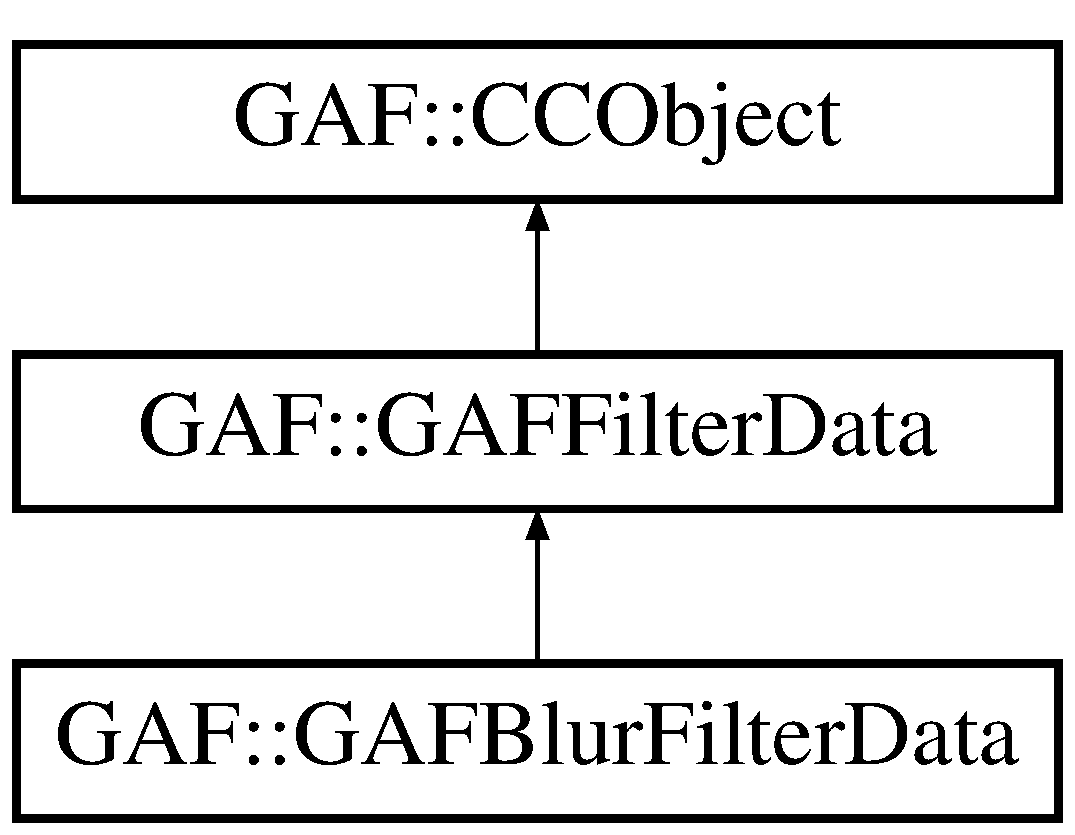
\includegraphics[height=3.000000cm]{class_g_a_f_1_1_g_a_f_filter_data}
\end{center}
\end{figure}
\subsection*{Additional Inherited Members}


The documentation for this class was generated from the following file\-:\begin{DoxyCompactItemize}
\item 
G\-A\-F\-Filter\-Data.\-h\end{DoxyCompactItemize}

\hypertarget{class_g_a_f_1_1_g_a_f_frame_played_delegate}{\section{G\-A\-F\-:\-:G\-A\-F\-Frame\-Played\-Delegate Class Reference}
\label{class_g_a_f_1_1_g_a_f_frame_played_delegate}\index{G\-A\-F\-::\-G\-A\-F\-Frame\-Played\-Delegate@{G\-A\-F\-::\-G\-A\-F\-Frame\-Played\-Delegate}}
}


{\ttfamily \#include $<$G\-A\-F\-Animated\-Object.\-h$>$}

\subsection*{Public Member Functions}
\begin{DoxyCompactItemize}
\item 
virtual void \hyperlink{class_g_a_f_1_1_g_a_f_frame_played_delegate_a46541dc98536863db94393b5673284e4}{on\-Frame\-Played} (\hyperlink{class_g_a_f_1_1_g_a_f_animated_object}{G\-A\-F\-Animated\-Object} $\ast$object, int frame)
\end{DoxyCompactItemize}


\subsection{Detailed Description}
You can get notification when particular frame of any \hyperlink{class_g_a_f_1_1_g_a_f_animated_object}{G\-A\-F\-Animated\-Object} is played. To do this you have to inherit \hyperlink{class_g_a_f_1_1_g_a_f_frame_played_delegate}{G\-A\-F\-Frame\-Played\-Delegate} and call set\-Frame\-Played\-Delegate method of your \hyperlink{class_g_a_f_1_1_g_a_f_animated_object}{G\-A\-F\-Animated\-Object} 

\subsection{Member Function Documentation}
\hypertarget{class_g_a_f_1_1_g_a_f_frame_played_delegate_a46541dc98536863db94393b5673284e4}{\index{G\-A\-F\-::\-G\-A\-F\-Frame\-Played\-Delegate@{G\-A\-F\-::\-G\-A\-F\-Frame\-Played\-Delegate}!on\-Frame\-Played@{on\-Frame\-Played}}
\index{on\-Frame\-Played@{on\-Frame\-Played}!GAF::GAFFramePlayedDelegate@{G\-A\-F\-::\-G\-A\-F\-Frame\-Played\-Delegate}}
\subsubsection[{on\-Frame\-Played}]{\setlength{\rightskip}{0pt plus 5cm}virtual void G\-A\-F\-::\-G\-A\-F\-Frame\-Played\-Delegate\-::on\-Frame\-Played (
\begin{DoxyParamCaption}
\item[{{\bf G\-A\-F\-Animated\-Object} $\ast$}]{object, }
\item[{int}]{frame}
\end{DoxyParamCaption}
)\hspace{0.3cm}{\ttfamily [virtual]}}}\label{class_g_a_f_1_1_g_a_f_frame_played_delegate_a46541dc98536863db94393b5673284e4}
Callback funtion, called by G\-A\-F. 
\begin{DoxyParams}{Parameters}
{\em object} & -\/ selected animated object \\
\hline
{\em frame} & -\/ frame number that is just played \\
\hline
\end{DoxyParams}


The documentation for this class was generated from the following file\-:\begin{DoxyCompactItemize}
\item 
G\-A\-F\-Animated\-Object.\-h\end{DoxyCompactItemize}

\hypertarget{class_g_a_f_1_1_g_a_f_interaction_object}{\section{G\-A\-F\-:\-:G\-A\-F\-Interaction\-Object Class Reference}
\label{class_g_a_f_1_1_g_a_f_interaction_object}\index{G\-A\-F\-::\-G\-A\-F\-Interaction\-Object@{G\-A\-F\-::\-G\-A\-F\-Interaction\-Object}}
}
Inheritance diagram for G\-A\-F\-:\-:G\-A\-F\-Interaction\-Object\-:\begin{figure}[H]
\begin{center}
\leavevmode
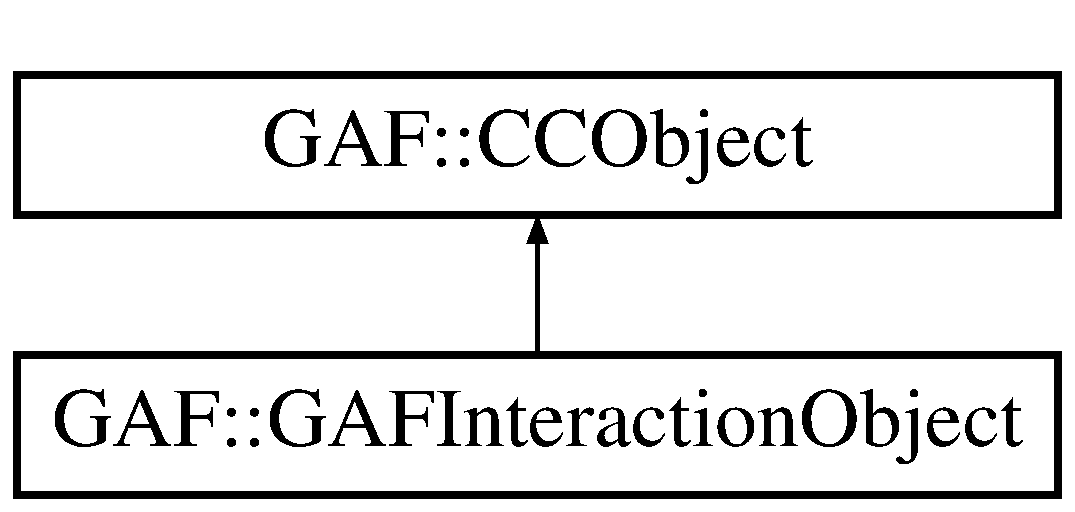
\includegraphics[height=2.000000cm]{class_g_a_f_1_1_g_a_f_interaction_object}
\end{center}
\end{figure}
\subsection*{Public Member Functions}
\begin{DoxyCompactItemize}
\item 
\hypertarget{class_g_a_f_1_1_g_a_f_interaction_object_aac8829b9b8f3b689a647394939ef72b2}{bool {\bfseries init\-With\-Dictionary} (\hyperlink{class_g_a_f_1_1_c_c_dictionary}{C\-C\-Dictionary} $\ast$a\-Dictionary)}\label{class_g_a_f_1_1_g_a_f_interaction_object_aac8829b9b8f3b689a647394939ef72b2}

\end{DoxyCompactItemize}
\subsection*{Static Public Member Functions}
\begin{DoxyCompactItemize}
\item 
\hypertarget{class_g_a_f_1_1_g_a_f_interaction_object_afa332acfa3fb81961619605d6cfb2854}{static \hyperlink{class_g_a_f_1_1_g_a_f_interaction_object}{G\-A\-F\-Interaction\-Object} $\ast$ {\bfseries create} (\hyperlink{class_g_a_f_1_1_c_c_dictionary}{C\-C\-Dictionary} $\ast$a\-Dictionary)}\label{class_g_a_f_1_1_g_a_f_interaction_object_afa332acfa3fb81961619605d6cfb2854}

\end{DoxyCompactItemize}
\subsection*{Public Attributes}
\begin{DoxyCompactItemize}
\item 
\hypertarget{class_g_a_f_1_1_g_a_f_interaction_object_a0086984dff9589d8d3c287039648ea13}{std\-::string {\bfseries name}}\label{class_g_a_f_1_1_g_a_f_interaction_object_a0086984dff9589d8d3c287039648ea13}

\item 
\hypertarget{class_g_a_f_1_1_g_a_f_interaction_object_a4f8c3543199eeacf9264e82bfba44b5c}{\hyperlink{class_g_a_f_1_1_c_c_point}{C\-C\-Point} {\bfseries pivot\-Point}}\label{class_g_a_f_1_1_g_a_f_interaction_object_a4f8c3543199eeacf9264e82bfba44b5c}

\item 
\hypertarget{class_g_a_f_1_1_g_a_f_interaction_object_a18458d08193fd96a8b189e5bd7543c61}{\hyperlink{class_g_a_f_1_1_c_c_rect}{C\-C\-Rect} {\bfseries bounds}}\label{class_g_a_f_1_1_g_a_f_interaction_object_a18458d08193fd96a8b189e5bd7543c61}

\end{DoxyCompactItemize}


The documentation for this class was generated from the following file\-:\begin{DoxyCompactItemize}
\item 
G\-A\-F\-Interaction\-Object.\-h\end{DoxyCompactItemize}

\hypertarget{class_g_a_f_1_1_g_a_f_marmalade_g_f_x}{\section{G\-A\-F\-:\-:G\-A\-F\-Marmalade\-G\-F\-X Class Reference}
\label{class_g_a_f_1_1_g_a_f_marmalade_g_f_x}\index{G\-A\-F\-::\-G\-A\-F\-Marmalade\-G\-F\-X@{G\-A\-F\-::\-G\-A\-F\-Marmalade\-G\-F\-X}}
}


{\ttfamily \#include $<$G\-A\-F\-Marmalade.\-h$>$}

\subsection*{Static Public Member Functions}
\begin{DoxyCompactItemize}
\item 
static void $\ast$ \hyperlink{class_g_a_f_1_1_g_a_f_marmalade_g_f_x_a3cf51925d3bcba812aa68d6f795776e8}{create\-Image} (const char $\ast$path)
\item 
static void \hyperlink{class_g_a_f_1_1_g_a_f_marmalade_g_f_x_a9170f1540e2d6672d76f18ed405f74e3}{release\-Image} (void $\ast$image)
\item 
static void $\ast$ \hyperlink{class_g_a_f_1_1_g_a_f_marmalade_g_f_x_a39395671c1920c67a28e5b0d83ade354}{create\-Texture} (void $\ast$image)
\item 
static void \hyperlink{class_g_a_f_1_1_g_a_f_marmalade_g_f_x_a1816b3f6a535721350373376256cb634}{release\-Texture} (void $\ast$texture)
\item 
\hypertarget{class_g_a_f_1_1_g_a_f_marmalade_g_f_x_a51f213df0e537a5994f89f66f93d8cbc}{static void $\ast$ \hyperlink{class_g_a_f_1_1_g_a_f_marmalade_g_f_x_a51f213df0e537a5994f89f66f93d8cbc}{create\-Sprite\-Container} ()}\label{class_g_a_f_1_1_g_a_f_marmalade_g_f_x_a51f213df0e537a5994f89f66f93d8cbc}

\begin{DoxyCompactList}\small\item\em You backend must have \char`\"{}sprite\-Container\char`\"{} abstraction. Most likely it is sprite itself. \end{DoxyCompactList}\item 
static void \hyperlink{class_g_a_f_1_1_g_a_f_marmalade_g_f_x_a7cd848f49d9aa6845a7c3d23b398b962}{release\-Sprite\-Container} (void $\ast$sprite\-Contaner)
\item 
static void \hyperlink{class_g_a_f_1_1_g_a_f_marmalade_g_f_x_a5ca22e99c8365ea12c844204b2a490ca}{set\-Sprite\-Container\-Scale} (void $\ast$sprite\-Contaner, float scale)
\item 
static void \hyperlink{class_g_a_f_1_1_g_a_f_marmalade_g_f_x_a0b97999d542ee4f2a303b0e62db74e86}{set\-Sprite\-Container\-Position} (void $\ast$sprte\-Container, float x, float y)
\item 
static void \hyperlink{class_g_a_f_1_1_g_a_f_marmalade_g_f_x_a99623ee7afb73f8b34ea38558d48d550}{set\-Sprite\-Position} (void $\ast$sprte, float x, float y)
\item 
static void \hyperlink{class_g_a_f_1_1_g_a_f_marmalade_g_f_x_a27662973702e6c78a2ea08d9b1a2f66e}{set\-Sprite\-Locator} (void $\ast$sprte, bool locator)
\item 
\hypertarget{class_g_a_f_1_1_g_a_f_marmalade_g_f_x_a532e1b916a435589f352be1d0fd64be1}{static void $\ast$ \hyperlink{class_g_a_f_1_1_g_a_f_marmalade_g_f_x_a532e1b916a435589f352be1d0fd64be1}{create\-Sprite} (\hyperlink{class_g_a_f_1_1_g_a_f_sprite_callback}{G\-A\-F\-::\-G\-A\-F\-Sprite\-Callback} $\ast$cb)}\label{class_g_a_f_1_1_g_a_f_marmalade_g_f_x_a532e1b916a435589f352be1d0fd64be1}

\begin{DoxyCompactList}\small\item\em You backend must have \char`\"{}sprite\char`\"{} abstraction. \end{DoxyCompactList}\item 
\hypertarget{class_g_a_f_1_1_g_a_f_marmalade_g_f_x_a8576303216810d7cf998033bbb448eb3}{static void $\ast$ \hyperlink{class_g_a_f_1_1_g_a_f_marmalade_g_f_x_a8576303216810d7cf998033bbb448eb3}{create\-Stencil\-Sprite} (\hyperlink{class_g_a_f_1_1_g_a_f_sprite_callback}{G\-A\-F\-::\-G\-A\-F\-Sprite\-Callback} $\ast$cb)}\label{class_g_a_f_1_1_g_a_f_marmalade_g_f_x_a8576303216810d7cf998033bbb448eb3}

\begin{DoxyCompactList}\small\item\em You backend must have \char`\"{}stencil sprite\char`\"{} abstraction. It must support masked objects. \end{DoxyCompactList}\item 
static void \hyperlink{class_g_a_f_1_1_g_a_f_marmalade_g_f_x_a549dc4e4ea1b208815a4efbb8fb3573d}{stencil\-Sprite\-Add\-Masked\-Object} (void $\ast$stencil\-Sprite, void $\ast$masked\-Object)
\item 
static void \hyperlink{class_g_a_f_1_1_g_a_f_marmalade_g_f_x_abc8a09dd883016053e10b31b6cdc4f5d}{stencil\-Sprite\-Update\-Mask\-Container\-Of} (void $\ast$stencil\-Sprite)
\item 
static bool \hyperlink{class_g_a_f_1_1_g_a_f_marmalade_g_f_x_a2026106206694ae8479daee70e25ac77}{init\-Sprite} (void $\ast$sprite, void $\ast$texture, float x, float y, float w, float h, bool rotated)
\item 
static void \hyperlink{class_g_a_f_1_1_g_a_f_marmalade_g_f_x_a6903462f1f840fff5a45312cda08c5e3}{release\-Sprite} (void $\ast$sprite)
\item 
static void \hyperlink{class_g_a_f_1_1_g_a_f_marmalade_g_f_x_accfa7a7c4665d5613a5c185603c2ae47}{set\-Sprite\-Transform} (void $\ast$sprite, const \hyperlink{class_g_a_f_1_1_c_c_affine_transform}{C\-C\-Affine\-Transform} \&transform)
\item 
static void $\ast$ \hyperlink{class_g_a_f_1_1_g_a_f_marmalade_g_f_x_aa85e3d2d9c75297bbadcb8f36beef8d7}{create\-Sprite\-Frame} (void $\ast$texture, float x, float y, float w, float h)
\item 
static void \hyperlink{class_g_a_f_1_1_g_a_f_marmalade_g_f_x_adc04e3b9f1e994a2bcebeadd88bd84ec}{release\-Sprite\-Frame} (void $\ast$sprite\-Frame)
\item 
static float \hyperlink{class_g_a_f_1_1_g_a_f_marmalade_g_f_x_a1cf7a56263c10187a2e154ba73c924f5}{get\-Sprite\-Content\-Size\-Width} (void $\ast$sprite)
\item 
static float \hyperlink{class_g_a_f_1_1_g_a_f_marmalade_g_f_x_a4820e51a219e807d0f1bf2f31faa7a4e}{get\-Sprite\-Content\-Size\-Height} (void $\ast$sprite)
\item 
static float \hyperlink{class_g_a_f_1_1_g_a_f_marmalade_g_f_x_a11fbebb5124bfc2a2f442eda4d0f8dc7}{get\-Sprite\-Anchor\-Position\-X} (void $\ast$sprite)
\item 
static float \hyperlink{class_g_a_f_1_1_g_a_f_marmalade_g_f_x_a77414124423838b04cd30cf983b7c664}{get\-Sprite\-Anchor\-Position\-Y} (void $\ast$sprite)
\item 
static int \hyperlink{class_g_a_f_1_1_g_a_f_marmalade_g_f_x_a66e33e99c61c1c32fd5335f7a563b42e}{get\-Sprite\-Zorder} (void $\ast$sprite)
\item 
static void \hyperlink{class_g_a_f_1_1_g_a_f_marmalade_g_f_x_a4094142fd3844a976e0ca03a5c64098f}{set\-Sprite\-Atlas\-Scale} (void $\ast$sprite, float scale)
\item 
static void $\ast$ \hyperlink{class_g_a_f_1_1_g_a_f_marmalade_g_f_x_a2b2282d1facfe40492e1d26ebc6c99dd}{get\-Sprite\-Parent} (void $\ast$sprite)
\item 
static void \hyperlink{class_g_a_f_1_1_g_a_f_marmalade_g_f_x_a5139d0f53eee9c67fa0995b1a8a2c9a4}{set\-Sprite\-Blur\-Radius} (void $\ast$sprite, float width, float height)
\item 
static void \hyperlink{class_g_a_f_1_1_g_a_f_marmalade_g_f_x_a64d246d6346ac1bd7de834894e92ba5a}{set\-Sprite\-Shader} (void $\ast$sprite, void $\ast$shader)
\item 
static void \hyperlink{class_g_a_f_1_1_g_a_f_marmalade_g_f_x_ad959554fc1cb14e8cf36efe269669d1f}{set\-Sprite\-Visible} (void $\ast$sprite, bool visible)
\item 
static void \hyperlink{class_g_a_f_1_1_g_a_f_marmalade_g_f_x_a5a12ea4b0fe453a0fc8dd46a3504bbe3}{set\-Sprite\-Anchor\-Point} (void $\ast$sprite, float x, float y)
\item 
static void \hyperlink{class_g_a_f_1_1_g_a_f_marmalade_g_f_x_aa1ee9a51e41aef8ef9ad197d80e51bfd}{set\-Sprite\-Zorder} (void $\ast$sprite, int z\-Order)
\item 
static void \hyperlink{class_g_a_f_1_1_g_a_f_marmalade_g_f_x_a97f7a8f2f82bcf2286cc3daaeec65046}{set\-Alpha\-Blending\-For\-Sprite} (void $\ast$sprite)
\item 
static void \hyperlink{class_g_a_f_1_1_g_a_f_marmalade_g_f_x_aad2b1d54954271b383655900c7a9b704}{set\-Sprite\-Container\-Zorder} (void $\ast$sprite\-Container, int z\-Order)
\item 
static void \hyperlink{class_g_a_f_1_1_g_a_f_marmalade_g_f_x_aa9306a997c52bb7b03ef2e13cf73297c}{scene\-Add\-Sprite\-Container} (void $\ast$scene, void $\ast$sprite\-Container)
\item 
static void \hyperlink{class_g_a_f_1_1_g_a_f_marmalade_g_f_x_a4e64e1c2a13125991357524949ea9472}{scene\-Remove\-Sprite\-Container} (void $\ast$scene, void $\ast$sprite\-Container)
\item 
static void \hyperlink{class_g_a_f_1_1_g_a_f_marmalade_g_f_x_a2f34d292870b7b7878665489873d5aaa}{sprite\-Container\-Add\-Sprite} (void $\ast$sprite\-Container, void $\ast$sprite)
\item 
static void \hyperlink{class_g_a_f_1_1_g_a_f_marmalade_g_f_x_a9834611e200459c3d0029caf080efd33}{sprite\-Container\-Remove\-Sprite} (void $\ast$sprite\-Container, void $\ast$sprite, bool cleanup)
\item 
static bool \hyperlink{class_g_a_f_1_1_g_a_f_marmalade_g_f_x_a948922dd8b7b9ae7bf4854cb81427ea4}{init\-Sprite\-With\-Sprite\-Frame} (void $\ast$sprite, void $\ast$sprite\-Frame)
\item 
\hypertarget{class_g_a_f_1_1_g_a_f_marmalade_g_f_x_acbe20a989f371ede8c045280f42d0b6d}{static void \hyperlink{class_g_a_f_1_1_g_a_f_marmalade_g_f_x_acbe20a989f371ede8c045280f42d0b6d}{schedule\-Update\-Per\-Frame} (\hyperlink{class_g_a_f_1_1_c_c_object}{C\-C\-Object} $\ast$object, G\-A\-F\-S\-E\-L\-\_\-\-Call\-Func)}\label{class_g_a_f_1_1_g_a_f_marmalade_g_f_x_acbe20a989f371ede8c045280f42d0b6d}

\begin{DoxyCompactList}\small\item\em used to update animations internally \end{DoxyCompactList}\item 
\hypertarget{class_g_a_f_1_1_g_a_f_marmalade_g_f_x_a85b396b19691358b7b1318eb65ed9c7a}{static void {\bfseries unschedule\-Update\-Per\-Frame} (\hyperlink{class_g_a_f_1_1_c_c_object}{C\-C\-Object} $\ast$object, G\-A\-F\-S\-E\-L\-\_\-\-Call\-Func)}\label{class_g_a_f_1_1_g_a_f_marmalade_g_f_x_a85b396b19691358b7b1318eb65ed9c7a}

\item 
\hypertarget{class_g_a_f_1_1_g_a_f_marmalade_g_f_x_a29a77c913497ddef3396f1e430ba428e}{static float \hyperlink{class_g_a_f_1_1_g_a_f_marmalade_g_f_x_a29a77c913497ddef3396f1e430ba428e}{get\-Animation\-Interval} ()}\label{class_g_a_f_1_1_g_a_f_marmalade_g_f_x_a29a77c913497ddef3396f1e430ba428e}

\begin{DoxyCompactList}\small\item\em used to get interval between frames in seconds \end{DoxyCompactList}\item 
static void \hyperlink{class_g_a_f_1_1_g_a_f_marmalade_g_f_x_a1c70fe78be6ca6ec191b38aa91c5fa44}{on\-Frame} ()
\end{DoxyCompactItemize}


\subsection{Detailed Description}
\begin{DoxyNote}{Note}
You must call \hyperlink{class_g_a_f_1_1_g_a_f_marmalade_g_f_x_a1c70fe78be6ca6ec191b38aa91c5fa44}{on\-Frame()} every frame after your rendering step is over or at the beginning of the frame.
\end{DoxyNote}
To implemnet rendering playback other than Cocos2dx you must implement all functions listed in \hyperlink{class_g_a_f_1_1_g_a_f_marmalade_g_f_x}{G\-A\-F\-Marmalade\-G\-F\-X}. For sample implementation you can check current Cocos2dx-\/bases implementation. Our advice is to contact gafmedia.\-com before you start to work on your own backend -\/ most likely backend you need is already in development. We tryed to be as less demanding as we can in terms of backend features you need to implement \hyperlink{class_g_a_f_1_1_g_a_f_marmalade_g_f_x}{G\-A\-F\-Marmalade\-G\-F\-X}. If your game engine features sprites, transformation and Open\-G\-L E\-S shaders it should not take too long to implement playback. If you have only Open\-G\-L E\-S immediate mode then things are more diffictult to you -\/ you have to implement mentioned abstructions. The most important thing with immediate mode implementation is carefully set and restore Open\-G\-L states. 

\subsection{Member Function Documentation}
\hypertarget{class_g_a_f_1_1_g_a_f_marmalade_g_f_x_a3cf51925d3bcba812aa68d6f795776e8}{\index{G\-A\-F\-::\-G\-A\-F\-Marmalade\-G\-F\-X@{G\-A\-F\-::\-G\-A\-F\-Marmalade\-G\-F\-X}!create\-Image@{create\-Image}}
\index{create\-Image@{create\-Image}!GAF::GAFMarmaladeGFX@{G\-A\-F\-::\-G\-A\-F\-Marmalade\-G\-F\-X}}
\subsubsection[{create\-Image}]{\setlength{\rightskip}{0pt plus 5cm}static void$\ast$ G\-A\-F\-::\-G\-A\-F\-Marmalade\-G\-F\-X\-::create\-Image (
\begin{DoxyParamCaption}
\item[{const char $\ast$}]{path}
\end{DoxyParamCaption}
)\hspace{0.3cm}{\ttfamily [static]}}}\label{class_g_a_f_1_1_g_a_f_marmalade_g_f_x_a3cf51925d3bcba812aa68d6f795776e8}
You backend must have \char`\"{}image\char`\"{} abstraction. 
\begin{DoxyParams}{Parameters}
{\em path} & -\/ resource path. This can be anything, but most likely it will be file system path. If you are going to do something else note that your code should respect image paths produced by G\-A\-F converter. \\
\hline
\end{DoxyParams}
\hypertarget{class_g_a_f_1_1_g_a_f_marmalade_g_f_x_aa85e3d2d9c75297bbadcb8f36beef8d7}{\index{G\-A\-F\-::\-G\-A\-F\-Marmalade\-G\-F\-X@{G\-A\-F\-::\-G\-A\-F\-Marmalade\-G\-F\-X}!create\-Sprite\-Frame@{create\-Sprite\-Frame}}
\index{create\-Sprite\-Frame@{create\-Sprite\-Frame}!GAF::GAFMarmaladeGFX@{G\-A\-F\-::\-G\-A\-F\-Marmalade\-G\-F\-X}}
\subsubsection[{create\-Sprite\-Frame}]{\setlength{\rightskip}{0pt plus 5cm}static void$\ast$ G\-A\-F\-::\-G\-A\-F\-Marmalade\-G\-F\-X\-::create\-Sprite\-Frame (
\begin{DoxyParamCaption}
\item[{void $\ast$}]{texture, }
\item[{float}]{x, }
\item[{float}]{y, }
\item[{float}]{w, }
\item[{float}]{h}
\end{DoxyParamCaption}
)\hspace{0.3cm}{\ttfamily [static]}}}\label{class_g_a_f_1_1_g_a_f_marmalade_g_f_x_aa85e3d2d9c75297bbadcb8f36beef8d7}
Your backend must have sprite frame abstraction. Basially it is just texture and texture rect. 
\begin{DoxyParams}{Parameters}
{\em texture} & -\/ created by \hyperlink{class_g_a_f_1_1_g_a_f_marmalade_g_f_x_a39395671c1920c67a28e5b0d83ade354}{G\-A\-F\-Marmalade\-G\-F\-X\-::create\-Texture} \\
\hline
{\em x,y,w,h} & -\/ texture rect \\
\hline
\end{DoxyParams}
\hypertarget{class_g_a_f_1_1_g_a_f_marmalade_g_f_x_a39395671c1920c67a28e5b0d83ade354}{\index{G\-A\-F\-::\-G\-A\-F\-Marmalade\-G\-F\-X@{G\-A\-F\-::\-G\-A\-F\-Marmalade\-G\-F\-X}!create\-Texture@{create\-Texture}}
\index{create\-Texture@{create\-Texture}!GAF::GAFMarmaladeGFX@{G\-A\-F\-::\-G\-A\-F\-Marmalade\-G\-F\-X}}
\subsubsection[{create\-Texture}]{\setlength{\rightskip}{0pt plus 5cm}static void$\ast$ G\-A\-F\-::\-G\-A\-F\-Marmalade\-G\-F\-X\-::create\-Texture (
\begin{DoxyParamCaption}
\item[{void $\ast$}]{image}
\end{DoxyParamCaption}
)\hspace{0.3cm}{\ttfamily [static]}}}\label{class_g_a_f_1_1_g_a_f_marmalade_g_f_x_a39395671c1920c67a28e5b0d83ade354}
You backend must have \char`\"{}texture\char`\"{} abstraction. 
\begin{DoxyParams}{Parameters}
{\em image} & -\/ image created by \hyperlink{class_g_a_f_1_1_g_a_f_marmalade_g_f_x_a3cf51925d3bcba812aa68d6f795776e8}{G\-A\-F\-Marmalade\-G\-F\-X\-::create\-Image} \\
\hline
\end{DoxyParams}
\hypertarget{class_g_a_f_1_1_g_a_f_marmalade_g_f_x_a11fbebb5124bfc2a2f442eda4d0f8dc7}{\index{G\-A\-F\-::\-G\-A\-F\-Marmalade\-G\-F\-X@{G\-A\-F\-::\-G\-A\-F\-Marmalade\-G\-F\-X}!get\-Sprite\-Anchor\-Position\-X@{get\-Sprite\-Anchor\-Position\-X}}
\index{get\-Sprite\-Anchor\-Position\-X@{get\-Sprite\-Anchor\-Position\-X}!GAF::GAFMarmaladeGFX@{G\-A\-F\-::\-G\-A\-F\-Marmalade\-G\-F\-X}}
\subsubsection[{get\-Sprite\-Anchor\-Position\-X}]{\setlength{\rightskip}{0pt plus 5cm}static float G\-A\-F\-::\-G\-A\-F\-Marmalade\-G\-F\-X\-::get\-Sprite\-Anchor\-Position\-X (
\begin{DoxyParamCaption}
\item[{void $\ast$}]{sprite}
\end{DoxyParamCaption}
)\hspace{0.3cm}{\ttfamily [static]}}}\label{class_g_a_f_1_1_g_a_f_marmalade_g_f_x_a11fbebb5124bfc2a2f442eda4d0f8dc7}

\begin{DoxyParams}{Parameters}
{\em sprite} & -\/ created by \hyperlink{class_g_a_f_1_1_g_a_f_marmalade_g_f_x_a532e1b916a435589f352be1d0fd64be1}{G\-A\-F\-Marmalade\-G\-F\-X\-::create\-Sprite} \\
\hline
\end{DoxyParams}
\begin{DoxyReturn}{Returns}
x position of sprite's anchor point 
\end{DoxyReturn}
\hypertarget{class_g_a_f_1_1_g_a_f_marmalade_g_f_x_a77414124423838b04cd30cf983b7c664}{\index{G\-A\-F\-::\-G\-A\-F\-Marmalade\-G\-F\-X@{G\-A\-F\-::\-G\-A\-F\-Marmalade\-G\-F\-X}!get\-Sprite\-Anchor\-Position\-Y@{get\-Sprite\-Anchor\-Position\-Y}}
\index{get\-Sprite\-Anchor\-Position\-Y@{get\-Sprite\-Anchor\-Position\-Y}!GAF::GAFMarmaladeGFX@{G\-A\-F\-::\-G\-A\-F\-Marmalade\-G\-F\-X}}
\subsubsection[{get\-Sprite\-Anchor\-Position\-Y}]{\setlength{\rightskip}{0pt plus 5cm}static float G\-A\-F\-::\-G\-A\-F\-Marmalade\-G\-F\-X\-::get\-Sprite\-Anchor\-Position\-Y (
\begin{DoxyParamCaption}
\item[{void $\ast$}]{sprite}
\end{DoxyParamCaption}
)\hspace{0.3cm}{\ttfamily [static]}}}\label{class_g_a_f_1_1_g_a_f_marmalade_g_f_x_a77414124423838b04cd30cf983b7c664}

\begin{DoxyParams}{Parameters}
{\em sprite} & -\/ created by \hyperlink{class_g_a_f_1_1_g_a_f_marmalade_g_f_x_a532e1b916a435589f352be1d0fd64be1}{G\-A\-F\-Marmalade\-G\-F\-X\-::create\-Sprite} \\
\hline
\end{DoxyParams}
\begin{DoxyReturn}{Returns}
y position of sprite's anchor point 
\end{DoxyReturn}
\hypertarget{class_g_a_f_1_1_g_a_f_marmalade_g_f_x_a4820e51a219e807d0f1bf2f31faa7a4e}{\index{G\-A\-F\-::\-G\-A\-F\-Marmalade\-G\-F\-X@{G\-A\-F\-::\-G\-A\-F\-Marmalade\-G\-F\-X}!get\-Sprite\-Content\-Size\-Height@{get\-Sprite\-Content\-Size\-Height}}
\index{get\-Sprite\-Content\-Size\-Height@{get\-Sprite\-Content\-Size\-Height}!GAF::GAFMarmaladeGFX@{G\-A\-F\-::\-G\-A\-F\-Marmalade\-G\-F\-X}}
\subsubsection[{get\-Sprite\-Content\-Size\-Height}]{\setlength{\rightskip}{0pt plus 5cm}static float G\-A\-F\-::\-G\-A\-F\-Marmalade\-G\-F\-X\-::get\-Sprite\-Content\-Size\-Height (
\begin{DoxyParamCaption}
\item[{void $\ast$}]{sprite}
\end{DoxyParamCaption}
)\hspace{0.3cm}{\ttfamily [static]}}}\label{class_g_a_f_1_1_g_a_f_marmalade_g_f_x_a4820e51a219e807d0f1bf2f31faa7a4e}

\begin{DoxyParams}{Parameters}
{\em sprite} & -\/ created by \hyperlink{class_g_a_f_1_1_g_a_f_marmalade_g_f_x_a532e1b916a435589f352be1d0fd64be1}{G\-A\-F\-Marmalade\-G\-F\-X\-::create\-Sprite} \\
\hline
\end{DoxyParams}
\begin{DoxyReturn}{Returns}
content size height 
\end{DoxyReturn}
\hypertarget{class_g_a_f_1_1_g_a_f_marmalade_g_f_x_a1cf7a56263c10187a2e154ba73c924f5}{\index{G\-A\-F\-::\-G\-A\-F\-Marmalade\-G\-F\-X@{G\-A\-F\-::\-G\-A\-F\-Marmalade\-G\-F\-X}!get\-Sprite\-Content\-Size\-Width@{get\-Sprite\-Content\-Size\-Width}}
\index{get\-Sprite\-Content\-Size\-Width@{get\-Sprite\-Content\-Size\-Width}!GAF::GAFMarmaladeGFX@{G\-A\-F\-::\-G\-A\-F\-Marmalade\-G\-F\-X}}
\subsubsection[{get\-Sprite\-Content\-Size\-Width}]{\setlength{\rightskip}{0pt plus 5cm}static float G\-A\-F\-::\-G\-A\-F\-Marmalade\-G\-F\-X\-::get\-Sprite\-Content\-Size\-Width (
\begin{DoxyParamCaption}
\item[{void $\ast$}]{sprite}
\end{DoxyParamCaption}
)\hspace{0.3cm}{\ttfamily [static]}}}\label{class_g_a_f_1_1_g_a_f_marmalade_g_f_x_a1cf7a56263c10187a2e154ba73c924f5}

\begin{DoxyParams}{Parameters}
{\em sprite} & -\/ created by \hyperlink{class_g_a_f_1_1_g_a_f_marmalade_g_f_x_a532e1b916a435589f352be1d0fd64be1}{G\-A\-F\-Marmalade\-G\-F\-X\-::create\-Sprite} \\
\hline
\end{DoxyParams}
\begin{DoxyReturn}{Returns}
content size width 
\end{DoxyReturn}
\hypertarget{class_g_a_f_1_1_g_a_f_marmalade_g_f_x_a2b2282d1facfe40492e1d26ebc6c99dd}{\index{G\-A\-F\-::\-G\-A\-F\-Marmalade\-G\-F\-X@{G\-A\-F\-::\-G\-A\-F\-Marmalade\-G\-F\-X}!get\-Sprite\-Parent@{get\-Sprite\-Parent}}
\index{get\-Sprite\-Parent@{get\-Sprite\-Parent}!GAF::GAFMarmaladeGFX@{G\-A\-F\-::\-G\-A\-F\-Marmalade\-G\-F\-X}}
\subsubsection[{get\-Sprite\-Parent}]{\setlength{\rightskip}{0pt plus 5cm}static void$\ast$ G\-A\-F\-::\-G\-A\-F\-Marmalade\-G\-F\-X\-::get\-Sprite\-Parent (
\begin{DoxyParamCaption}
\item[{void $\ast$}]{sprite}
\end{DoxyParamCaption}
)\hspace{0.3cm}{\ttfamily [static]}}}\label{class_g_a_f_1_1_g_a_f_marmalade_g_f_x_a2b2282d1facfe40492e1d26ebc6c99dd}

\begin{DoxyParams}{Parameters}
{\em sprite} & -\/ created by \hyperlink{class_g_a_f_1_1_g_a_f_marmalade_g_f_x_a532e1b916a435589f352be1d0fd64be1}{G\-A\-F\-Marmalade\-G\-F\-X\-::create\-Sprite} \\
\hline
\end{DoxyParams}
\hypertarget{class_g_a_f_1_1_g_a_f_marmalade_g_f_x_a66e33e99c61c1c32fd5335f7a563b42e}{\index{G\-A\-F\-::\-G\-A\-F\-Marmalade\-G\-F\-X@{G\-A\-F\-::\-G\-A\-F\-Marmalade\-G\-F\-X}!get\-Sprite\-Zorder@{get\-Sprite\-Zorder}}
\index{get\-Sprite\-Zorder@{get\-Sprite\-Zorder}!GAF::GAFMarmaladeGFX@{G\-A\-F\-::\-G\-A\-F\-Marmalade\-G\-F\-X}}
\subsubsection[{get\-Sprite\-Zorder}]{\setlength{\rightskip}{0pt plus 5cm}static int G\-A\-F\-::\-G\-A\-F\-Marmalade\-G\-F\-X\-::get\-Sprite\-Zorder (
\begin{DoxyParamCaption}
\item[{void $\ast$}]{sprite}
\end{DoxyParamCaption}
)\hspace{0.3cm}{\ttfamily [static]}}}\label{class_g_a_f_1_1_g_a_f_marmalade_g_f_x_a66e33e99c61c1c32fd5335f7a563b42e}

\begin{DoxyParams}{Parameters}
{\em sprite} & -\/ created by \hyperlink{class_g_a_f_1_1_g_a_f_marmalade_g_f_x_a532e1b916a435589f352be1d0fd64be1}{G\-A\-F\-Marmalade\-G\-F\-X\-::create\-Sprite} \\
\hline
\end{DoxyParams}
\begin{DoxyReturn}{Returns}
z order of the sprite 
\end{DoxyReturn}
\hypertarget{class_g_a_f_1_1_g_a_f_marmalade_g_f_x_a2026106206694ae8479daee70e25ac77}{\index{G\-A\-F\-::\-G\-A\-F\-Marmalade\-G\-F\-X@{G\-A\-F\-::\-G\-A\-F\-Marmalade\-G\-F\-X}!init\-Sprite@{init\-Sprite}}
\index{init\-Sprite@{init\-Sprite}!GAF::GAFMarmaladeGFX@{G\-A\-F\-::\-G\-A\-F\-Marmalade\-G\-F\-X}}
\subsubsection[{init\-Sprite}]{\setlength{\rightskip}{0pt plus 5cm}static bool G\-A\-F\-::\-G\-A\-F\-Marmalade\-G\-F\-X\-::init\-Sprite (
\begin{DoxyParamCaption}
\item[{void $\ast$}]{sprite, }
\item[{void $\ast$}]{texture, }
\item[{float}]{x, }
\item[{float}]{y, }
\item[{float}]{w, }
\item[{float}]{h, }
\item[{bool}]{rotated}
\end{DoxyParamCaption}
)\hspace{0.3cm}{\ttfamily [static]}}}\label{class_g_a_f_1_1_g_a_f_marmalade_g_f_x_a2026106206694ae8479daee70e25ac77}
Sprite initialization 
\begin{DoxyParams}{Parameters}
{\em sprite} & -\/ created by \hyperlink{class_g_a_f_1_1_g_a_f_marmalade_g_f_x_a532e1b916a435589f352be1d0fd64be1}{G\-A\-F\-Marmalade\-G\-F\-X\-::create\-Sprite} \\
\hline
{\em texture} & -\/ created by \hyperlink{class_g_a_f_1_1_g_a_f_marmalade_g_f_x_a39395671c1920c67a28e5b0d83ade354}{G\-A\-F\-Marmalade\-G\-F\-X\-::create\-Texture} \\
\hline
{\em x,y,w,h} & -\/ sprite rect \\
\hline
{\em rotated} & -\/ if sprite rect rotated or not \\
\hline
\end{DoxyParams}
\hypertarget{class_g_a_f_1_1_g_a_f_marmalade_g_f_x_a948922dd8b7b9ae7bf4854cb81427ea4}{\index{G\-A\-F\-::\-G\-A\-F\-Marmalade\-G\-F\-X@{G\-A\-F\-::\-G\-A\-F\-Marmalade\-G\-F\-X}!init\-Sprite\-With\-Sprite\-Frame@{init\-Sprite\-With\-Sprite\-Frame}}
\index{init\-Sprite\-With\-Sprite\-Frame@{init\-Sprite\-With\-Sprite\-Frame}!GAF::GAFMarmaladeGFX@{G\-A\-F\-::\-G\-A\-F\-Marmalade\-G\-F\-X}}
\subsubsection[{init\-Sprite\-With\-Sprite\-Frame}]{\setlength{\rightskip}{0pt plus 5cm}static bool G\-A\-F\-::\-G\-A\-F\-Marmalade\-G\-F\-X\-::init\-Sprite\-With\-Sprite\-Frame (
\begin{DoxyParamCaption}
\item[{void $\ast$}]{sprite, }
\item[{void $\ast$}]{sprite\-Frame}
\end{DoxyParamCaption}
)\hspace{0.3cm}{\ttfamily [static]}}}\label{class_g_a_f_1_1_g_a_f_marmalade_g_f_x_a948922dd8b7b9ae7bf4854cb81427ea4}

\begin{DoxyParams}{Parameters}
{\em sprite} & -\/ created by \hyperlink{class_g_a_f_1_1_g_a_f_marmalade_g_f_x_a532e1b916a435589f352be1d0fd64be1}{G\-A\-F\-Marmalade\-G\-F\-X\-::create\-Sprite} \\
\hline
{\em sprite\-Frame} & -\/ created by \hyperlink{class_g_a_f_1_1_g_a_f_marmalade_g_f_x_aa85e3d2d9c75297bbadcb8f36beef8d7}{G\-A\-F\-Marmalade\-G\-F\-X\-::create\-Sprite\-Frame} \\
\hline
\end{DoxyParams}
\hypertarget{class_g_a_f_1_1_g_a_f_marmalade_g_f_x_a1c70fe78be6ca6ec191b38aa91c5fa44}{\index{G\-A\-F\-::\-G\-A\-F\-Marmalade\-G\-F\-X@{G\-A\-F\-::\-G\-A\-F\-Marmalade\-G\-F\-X}!on\-Frame@{on\-Frame}}
\index{on\-Frame@{on\-Frame}!GAF::GAFMarmaladeGFX@{G\-A\-F\-::\-G\-A\-F\-Marmalade\-G\-F\-X}}
\subsubsection[{on\-Frame}]{\setlength{\rightskip}{0pt plus 5cm}static void G\-A\-F\-::\-G\-A\-F\-Marmalade\-G\-F\-X\-::on\-Frame (
\begin{DoxyParamCaption}
{}
\end{DoxyParamCaption}
)\hspace{0.3cm}{\ttfamily [static]}}}\label{class_g_a_f_1_1_g_a_f_marmalade_g_f_x_a1c70fe78be6ca6ec191b38aa91c5fa44}
\begin{DoxyNote}{Note}
You must call \hyperlink{class_g_a_f_1_1_g_a_f_marmalade_g_f_x_a1c70fe78be6ca6ec191b38aa91c5fa44}{on\-Frame()} every frame after your rendering step is over or at the beginning of the frame. 
\end{DoxyNote}
\hypertarget{class_g_a_f_1_1_g_a_f_marmalade_g_f_x_a9170f1540e2d6672d76f18ed405f74e3}{\index{G\-A\-F\-::\-G\-A\-F\-Marmalade\-G\-F\-X@{G\-A\-F\-::\-G\-A\-F\-Marmalade\-G\-F\-X}!release\-Image@{release\-Image}}
\index{release\-Image@{release\-Image}!GAF::GAFMarmaladeGFX@{G\-A\-F\-::\-G\-A\-F\-Marmalade\-G\-F\-X}}
\subsubsection[{release\-Image}]{\setlength{\rightskip}{0pt plus 5cm}static void G\-A\-F\-::\-G\-A\-F\-Marmalade\-G\-F\-X\-::release\-Image (
\begin{DoxyParamCaption}
\item[{void $\ast$}]{image}
\end{DoxyParamCaption}
)\hspace{0.3cm}{\ttfamily [static]}}}\label{class_g_a_f_1_1_g_a_f_marmalade_g_f_x_a9170f1540e2d6672d76f18ed405f74e3}

\begin{DoxyParams}{Parameters}
{\em image} & -\/ created by \hyperlink{class_g_a_f_1_1_g_a_f_marmalade_g_f_x_a3cf51925d3bcba812aa68d6f795776e8}{G\-A\-F\-Marmalade\-G\-F\-X\-::create\-Image} \\
\hline
\end{DoxyParams}
\hypertarget{class_g_a_f_1_1_g_a_f_marmalade_g_f_x_a6903462f1f840fff5a45312cda08c5e3}{\index{G\-A\-F\-::\-G\-A\-F\-Marmalade\-G\-F\-X@{G\-A\-F\-::\-G\-A\-F\-Marmalade\-G\-F\-X}!release\-Sprite@{release\-Sprite}}
\index{release\-Sprite@{release\-Sprite}!GAF::GAFMarmaladeGFX@{G\-A\-F\-::\-G\-A\-F\-Marmalade\-G\-F\-X}}
\subsubsection[{release\-Sprite}]{\setlength{\rightskip}{0pt plus 5cm}static void G\-A\-F\-::\-G\-A\-F\-Marmalade\-G\-F\-X\-::release\-Sprite (
\begin{DoxyParamCaption}
\item[{void $\ast$}]{sprite}
\end{DoxyParamCaption}
)\hspace{0.3cm}{\ttfamily [static]}}}\label{class_g_a_f_1_1_g_a_f_marmalade_g_f_x_a6903462f1f840fff5a45312cda08c5e3}

\begin{DoxyParams}{Parameters}
{\em sprite} & -\/ created by create\-Sprite \\
\hline
\end{DoxyParams}
\hypertarget{class_g_a_f_1_1_g_a_f_marmalade_g_f_x_a7cd848f49d9aa6845a7c3d23b398b962}{\index{G\-A\-F\-::\-G\-A\-F\-Marmalade\-G\-F\-X@{G\-A\-F\-::\-G\-A\-F\-Marmalade\-G\-F\-X}!release\-Sprite\-Container@{release\-Sprite\-Container}}
\index{release\-Sprite\-Container@{release\-Sprite\-Container}!GAF::GAFMarmaladeGFX@{G\-A\-F\-::\-G\-A\-F\-Marmalade\-G\-F\-X}}
\subsubsection[{release\-Sprite\-Container}]{\setlength{\rightskip}{0pt plus 5cm}static void G\-A\-F\-::\-G\-A\-F\-Marmalade\-G\-F\-X\-::release\-Sprite\-Container (
\begin{DoxyParamCaption}
\item[{void $\ast$}]{sprite\-Contaner}
\end{DoxyParamCaption}
)\hspace{0.3cm}{\ttfamily [static]}}}\label{class_g_a_f_1_1_g_a_f_marmalade_g_f_x_a7cd848f49d9aa6845a7c3d23b398b962}

\begin{DoxyParams}{Parameters}
{\em sprite\-Contaner} & -\/ create by \hyperlink{class_g_a_f_1_1_g_a_f_marmalade_g_f_x_a51f213df0e537a5994f89f66f93d8cbc}{G\-A\-F\-Marmalade\-G\-F\-X\-::create\-Sprite\-Container} \\
\hline
\end{DoxyParams}
\hypertarget{class_g_a_f_1_1_g_a_f_marmalade_g_f_x_adc04e3b9f1e994a2bcebeadd88bd84ec}{\index{G\-A\-F\-::\-G\-A\-F\-Marmalade\-G\-F\-X@{G\-A\-F\-::\-G\-A\-F\-Marmalade\-G\-F\-X}!release\-Sprite\-Frame@{release\-Sprite\-Frame}}
\index{release\-Sprite\-Frame@{release\-Sprite\-Frame}!GAF::GAFMarmaladeGFX@{G\-A\-F\-::\-G\-A\-F\-Marmalade\-G\-F\-X}}
\subsubsection[{release\-Sprite\-Frame}]{\setlength{\rightskip}{0pt plus 5cm}static void G\-A\-F\-::\-G\-A\-F\-Marmalade\-G\-F\-X\-::release\-Sprite\-Frame (
\begin{DoxyParamCaption}
\item[{void $\ast$}]{sprite\-Frame}
\end{DoxyParamCaption}
)\hspace{0.3cm}{\ttfamily [static]}}}\label{class_g_a_f_1_1_g_a_f_marmalade_g_f_x_adc04e3b9f1e994a2bcebeadd88bd84ec}

\begin{DoxyParams}{Parameters}
{\em sprite\-Frame} & -\/ created by \hyperlink{class_g_a_f_1_1_g_a_f_marmalade_g_f_x_aa85e3d2d9c75297bbadcb8f36beef8d7}{G\-A\-F\-Marmalade\-G\-F\-X\-::create\-Sprite\-Frame} \\
\hline
\end{DoxyParams}
\hypertarget{class_g_a_f_1_1_g_a_f_marmalade_g_f_x_a1816b3f6a535721350373376256cb634}{\index{G\-A\-F\-::\-G\-A\-F\-Marmalade\-G\-F\-X@{G\-A\-F\-::\-G\-A\-F\-Marmalade\-G\-F\-X}!release\-Texture@{release\-Texture}}
\index{release\-Texture@{release\-Texture}!GAF::GAFMarmaladeGFX@{G\-A\-F\-::\-G\-A\-F\-Marmalade\-G\-F\-X}}
\subsubsection[{release\-Texture}]{\setlength{\rightskip}{0pt plus 5cm}static void G\-A\-F\-::\-G\-A\-F\-Marmalade\-G\-F\-X\-::release\-Texture (
\begin{DoxyParamCaption}
\item[{void $\ast$}]{texture}
\end{DoxyParamCaption}
)\hspace{0.3cm}{\ttfamily [static]}}}\label{class_g_a_f_1_1_g_a_f_marmalade_g_f_x_a1816b3f6a535721350373376256cb634}

\begin{DoxyParams}{Parameters}
{\em texture} & -\/ created by \hyperlink{class_g_a_f_1_1_g_a_f_marmalade_g_f_x_a39395671c1920c67a28e5b0d83ade354}{G\-A\-F\-Marmalade\-G\-F\-X\-::create\-Texture} \\
\hline
\end{DoxyParams}
\hypertarget{class_g_a_f_1_1_g_a_f_marmalade_g_f_x_aa9306a997c52bb7b03ef2e13cf73297c}{\index{G\-A\-F\-::\-G\-A\-F\-Marmalade\-G\-F\-X@{G\-A\-F\-::\-G\-A\-F\-Marmalade\-G\-F\-X}!scene\-Add\-Sprite\-Container@{scene\-Add\-Sprite\-Container}}
\index{scene\-Add\-Sprite\-Container@{scene\-Add\-Sprite\-Container}!GAF::GAFMarmaladeGFX@{G\-A\-F\-::\-G\-A\-F\-Marmalade\-G\-F\-X}}
\subsubsection[{scene\-Add\-Sprite\-Container}]{\setlength{\rightskip}{0pt plus 5cm}static void G\-A\-F\-::\-G\-A\-F\-Marmalade\-G\-F\-X\-::scene\-Add\-Sprite\-Container (
\begin{DoxyParamCaption}
\item[{void $\ast$}]{scene, }
\item[{void $\ast$}]{sprite\-Container}
\end{DoxyParamCaption}
)\hspace{0.3cm}{\ttfamily [static]}}}\label{class_g_a_f_1_1_g_a_f_marmalade_g_f_x_aa9306a997c52bb7b03ef2e13cf73297c}
adds sprite container to scene 
\begin{DoxyParams}{Parameters}
{\em scene} & -\/ object that can contin sprite containers. \\
\hline
{\em sprite\-Container} & -\/ created by \hyperlink{class_g_a_f_1_1_g_a_f_marmalade_g_f_x_a51f213df0e537a5994f89f66f93d8cbc}{G\-A\-F\-Marmalade\-G\-F\-X\-::create\-Sprite\-Container} \\
\hline
\end{DoxyParams}
\hypertarget{class_g_a_f_1_1_g_a_f_marmalade_g_f_x_a4e64e1c2a13125991357524949ea9472}{\index{G\-A\-F\-::\-G\-A\-F\-Marmalade\-G\-F\-X@{G\-A\-F\-::\-G\-A\-F\-Marmalade\-G\-F\-X}!scene\-Remove\-Sprite\-Container@{scene\-Remove\-Sprite\-Container}}
\index{scene\-Remove\-Sprite\-Container@{scene\-Remove\-Sprite\-Container}!GAF::GAFMarmaladeGFX@{G\-A\-F\-::\-G\-A\-F\-Marmalade\-G\-F\-X}}
\subsubsection[{scene\-Remove\-Sprite\-Container}]{\setlength{\rightskip}{0pt plus 5cm}static void G\-A\-F\-::\-G\-A\-F\-Marmalade\-G\-F\-X\-::scene\-Remove\-Sprite\-Container (
\begin{DoxyParamCaption}
\item[{void $\ast$}]{scene, }
\item[{void $\ast$}]{sprite\-Container}
\end{DoxyParamCaption}
)\hspace{0.3cm}{\ttfamily [static]}}}\label{class_g_a_f_1_1_g_a_f_marmalade_g_f_x_a4e64e1c2a13125991357524949ea9472}
removes sprite container from scene 
\begin{DoxyParams}{Parameters}
{\em scene} & -\/ object that can contin sprite containers. \\
\hline
{\em sprite\-Container} & -\/ created by \hyperlink{class_g_a_f_1_1_g_a_f_marmalade_g_f_x_a51f213df0e537a5994f89f66f93d8cbc}{G\-A\-F\-Marmalade\-G\-F\-X\-::create\-Sprite\-Container} \\
\hline
\end{DoxyParams}
\hypertarget{class_g_a_f_1_1_g_a_f_marmalade_g_f_x_a97f7a8f2f82bcf2286cc3daaeec65046}{\index{G\-A\-F\-::\-G\-A\-F\-Marmalade\-G\-F\-X@{G\-A\-F\-::\-G\-A\-F\-Marmalade\-G\-F\-X}!set\-Alpha\-Blending\-For\-Sprite@{set\-Alpha\-Blending\-For\-Sprite}}
\index{set\-Alpha\-Blending\-For\-Sprite@{set\-Alpha\-Blending\-For\-Sprite}!GAF::GAFMarmaladeGFX@{G\-A\-F\-::\-G\-A\-F\-Marmalade\-G\-F\-X}}
\subsubsection[{set\-Alpha\-Blending\-For\-Sprite}]{\setlength{\rightskip}{0pt plus 5cm}static void G\-A\-F\-::\-G\-A\-F\-Marmalade\-G\-F\-X\-::set\-Alpha\-Blending\-For\-Sprite (
\begin{DoxyParamCaption}
\item[{void $\ast$}]{sprite}
\end{DoxyParamCaption}
)\hspace{0.3cm}{\ttfamily [static]}}}\label{class_g_a_f_1_1_g_a_f_marmalade_g_f_x_a97f7a8f2f82bcf2286cc3daaeec65046}
Must set parameters that are equivalent to the following \-: src -\/ O\-N\-E dst -\/ O\-N\-E\-\_\-\-M\-I\-N\-U\-S\-\_\-\-S\-R\-C\-\_\-\-A\-L\-P\-H\-A 
\begin{DoxyParams}{Parameters}
{\em sprite} & -\/ created by \hyperlink{class_g_a_f_1_1_g_a_f_marmalade_g_f_x_a532e1b916a435589f352be1d0fd64be1}{G\-A\-F\-Marmalade\-G\-F\-X\-::create\-Sprite} \\
\hline
\end{DoxyParams}
\hypertarget{class_g_a_f_1_1_g_a_f_marmalade_g_f_x_a5a12ea4b0fe453a0fc8dd46a3504bbe3}{\index{G\-A\-F\-::\-G\-A\-F\-Marmalade\-G\-F\-X@{G\-A\-F\-::\-G\-A\-F\-Marmalade\-G\-F\-X}!set\-Sprite\-Anchor\-Point@{set\-Sprite\-Anchor\-Point}}
\index{set\-Sprite\-Anchor\-Point@{set\-Sprite\-Anchor\-Point}!GAF::GAFMarmaladeGFX@{G\-A\-F\-::\-G\-A\-F\-Marmalade\-G\-F\-X}}
\subsubsection[{set\-Sprite\-Anchor\-Point}]{\setlength{\rightskip}{0pt plus 5cm}static void G\-A\-F\-::\-G\-A\-F\-Marmalade\-G\-F\-X\-::set\-Sprite\-Anchor\-Point (
\begin{DoxyParamCaption}
\item[{void $\ast$}]{sprite, }
\item[{float}]{x, }
\item[{float}]{y}
\end{DoxyParamCaption}
)\hspace{0.3cm}{\ttfamily [static]}}}\label{class_g_a_f_1_1_g_a_f_marmalade_g_f_x_a5a12ea4b0fe453a0fc8dd46a3504bbe3}

\begin{DoxyParams}{Parameters}
{\em sprite} & -\/ created by \hyperlink{class_g_a_f_1_1_g_a_f_marmalade_g_f_x_a532e1b916a435589f352be1d0fd64be1}{G\-A\-F\-Marmalade\-G\-F\-X\-::create\-Sprite} \\
\hline
{\em x,y} & -\/ ahchor point \\
\hline
\end{DoxyParams}
\hypertarget{class_g_a_f_1_1_g_a_f_marmalade_g_f_x_a4094142fd3844a976e0ca03a5c64098f}{\index{G\-A\-F\-::\-G\-A\-F\-Marmalade\-G\-F\-X@{G\-A\-F\-::\-G\-A\-F\-Marmalade\-G\-F\-X}!set\-Sprite\-Atlas\-Scale@{set\-Sprite\-Atlas\-Scale}}
\index{set\-Sprite\-Atlas\-Scale@{set\-Sprite\-Atlas\-Scale}!GAF::GAFMarmaladeGFX@{G\-A\-F\-::\-G\-A\-F\-Marmalade\-G\-F\-X}}
\subsubsection[{set\-Sprite\-Atlas\-Scale}]{\setlength{\rightskip}{0pt plus 5cm}static void G\-A\-F\-::\-G\-A\-F\-Marmalade\-G\-F\-X\-::set\-Sprite\-Atlas\-Scale (
\begin{DoxyParamCaption}
\item[{void $\ast$}]{sprite, }
\item[{float}]{scale}
\end{DoxyParamCaption}
)\hspace{0.3cm}{\ttfamily [static]}}}\label{class_g_a_f_1_1_g_a_f_marmalade_g_f_x_a4094142fd3844a976e0ca03a5c64098f}
set G\-A\-F atlas scale of the sprite 
\begin{DoxyParams}{Parameters}
{\em sprite} & -\/ created by \hyperlink{class_g_a_f_1_1_g_a_f_marmalade_g_f_x_a532e1b916a435589f352be1d0fd64be1}{G\-A\-F\-Marmalade\-G\-F\-X\-::create\-Sprite} \\
\hline
\end{DoxyParams}
\hypertarget{class_g_a_f_1_1_g_a_f_marmalade_g_f_x_a5139d0f53eee9c67fa0995b1a8a2c9a4}{\index{G\-A\-F\-::\-G\-A\-F\-Marmalade\-G\-F\-X@{G\-A\-F\-::\-G\-A\-F\-Marmalade\-G\-F\-X}!set\-Sprite\-Blur\-Radius@{set\-Sprite\-Blur\-Radius}}
\index{set\-Sprite\-Blur\-Radius@{set\-Sprite\-Blur\-Radius}!GAF::GAFMarmaladeGFX@{G\-A\-F\-::\-G\-A\-F\-Marmalade\-G\-F\-X}}
\subsubsection[{set\-Sprite\-Blur\-Radius}]{\setlength{\rightskip}{0pt plus 5cm}static void G\-A\-F\-::\-G\-A\-F\-Marmalade\-G\-F\-X\-::set\-Sprite\-Blur\-Radius (
\begin{DoxyParamCaption}
\item[{void $\ast$}]{sprite, }
\item[{float}]{width, }
\item[{float}]{height}
\end{DoxyParamCaption}
)\hspace{0.3cm}{\ttfamily [static]}}}\label{class_g_a_f_1_1_g_a_f_marmalade_g_f_x_a5139d0f53eee9c67fa0995b1a8a2c9a4}

\begin{DoxyParams}{Parameters}
{\em sprite} & -\/ created by \hyperlink{class_g_a_f_1_1_g_a_f_marmalade_g_f_x_a532e1b916a435589f352be1d0fd64be1}{G\-A\-F\-Marmalade\-G\-F\-X\-::create\-Sprite} \\
\hline
\end{DoxyParams}
\hypertarget{class_g_a_f_1_1_g_a_f_marmalade_g_f_x_a0b97999d542ee4f2a303b0e62db74e86}{\index{G\-A\-F\-::\-G\-A\-F\-Marmalade\-G\-F\-X@{G\-A\-F\-::\-G\-A\-F\-Marmalade\-G\-F\-X}!set\-Sprite\-Container\-Position@{set\-Sprite\-Container\-Position}}
\index{set\-Sprite\-Container\-Position@{set\-Sprite\-Container\-Position}!GAF::GAFMarmaladeGFX@{G\-A\-F\-::\-G\-A\-F\-Marmalade\-G\-F\-X}}
\subsubsection[{set\-Sprite\-Container\-Position}]{\setlength{\rightskip}{0pt plus 5cm}static void G\-A\-F\-::\-G\-A\-F\-Marmalade\-G\-F\-X\-::set\-Sprite\-Container\-Position (
\begin{DoxyParamCaption}
\item[{void $\ast$}]{sprte\-Container, }
\item[{float}]{x, }
\item[{float}]{y}
\end{DoxyParamCaption}
)\hspace{0.3cm}{\ttfamily [static]}}}\label{class_g_a_f_1_1_g_a_f_marmalade_g_f_x_a0b97999d542ee4f2a303b0e62db74e86}
\begin{DoxyNote}{Note}
sprites located in sprite continer must respect parent's position 
\end{DoxyNote}
\hypertarget{class_g_a_f_1_1_g_a_f_marmalade_g_f_x_a5ca22e99c8365ea12c844204b2a490ca}{\index{G\-A\-F\-::\-G\-A\-F\-Marmalade\-G\-F\-X@{G\-A\-F\-::\-G\-A\-F\-Marmalade\-G\-F\-X}!set\-Sprite\-Container\-Scale@{set\-Sprite\-Container\-Scale}}
\index{set\-Sprite\-Container\-Scale@{set\-Sprite\-Container\-Scale}!GAF::GAFMarmaladeGFX@{G\-A\-F\-::\-G\-A\-F\-Marmalade\-G\-F\-X}}
\subsubsection[{set\-Sprite\-Container\-Scale}]{\setlength{\rightskip}{0pt plus 5cm}static void G\-A\-F\-::\-G\-A\-F\-Marmalade\-G\-F\-X\-::set\-Sprite\-Container\-Scale (
\begin{DoxyParamCaption}
\item[{void $\ast$}]{sprite\-Contaner, }
\item[{float}]{scale}
\end{DoxyParamCaption}
)\hspace{0.3cm}{\ttfamily [static]}}}\label{class_g_a_f_1_1_g_a_f_marmalade_g_f_x_a5ca22e99c8365ea12c844204b2a490ca}
\begin{DoxyNote}{Note}
sprites located in sprite continer must respect parent's scale 
\end{DoxyNote}
\hypertarget{class_g_a_f_1_1_g_a_f_marmalade_g_f_x_aad2b1d54954271b383655900c7a9b704}{\index{G\-A\-F\-::\-G\-A\-F\-Marmalade\-G\-F\-X@{G\-A\-F\-::\-G\-A\-F\-Marmalade\-G\-F\-X}!set\-Sprite\-Container\-Zorder@{set\-Sprite\-Container\-Zorder}}
\index{set\-Sprite\-Container\-Zorder@{set\-Sprite\-Container\-Zorder}!GAF::GAFMarmaladeGFX@{G\-A\-F\-::\-G\-A\-F\-Marmalade\-G\-F\-X}}
\subsubsection[{set\-Sprite\-Container\-Zorder}]{\setlength{\rightskip}{0pt plus 5cm}static void G\-A\-F\-::\-G\-A\-F\-Marmalade\-G\-F\-X\-::set\-Sprite\-Container\-Zorder (
\begin{DoxyParamCaption}
\item[{void $\ast$}]{sprite\-Container, }
\item[{int}]{z\-Order}
\end{DoxyParamCaption}
)\hspace{0.3cm}{\ttfamily [static]}}}\label{class_g_a_f_1_1_g_a_f_marmalade_g_f_x_aad2b1d54954271b383655900c7a9b704}

\begin{DoxyParams}{Parameters}
{\em sprite\-Container} & -\/ created by \hyperlink{class_g_a_f_1_1_g_a_f_marmalade_g_f_x_a51f213df0e537a5994f89f66f93d8cbc}{G\-A\-F\-Marmalade\-G\-F\-X\-::create\-Sprite\-Container} \\
\hline
{\em z\-Order} & -\/ z order \\
\hline
\end{DoxyParams}
\hypertarget{class_g_a_f_1_1_g_a_f_marmalade_g_f_x_a27662973702e6c78a2ea08d9b1a2f66e}{\index{G\-A\-F\-::\-G\-A\-F\-Marmalade\-G\-F\-X@{G\-A\-F\-::\-G\-A\-F\-Marmalade\-G\-F\-X}!set\-Sprite\-Locator@{set\-Sprite\-Locator}}
\index{set\-Sprite\-Locator@{set\-Sprite\-Locator}!GAF::GAFMarmaladeGFX@{G\-A\-F\-::\-G\-A\-F\-Marmalade\-G\-F\-X}}
\subsubsection[{set\-Sprite\-Locator}]{\setlength{\rightskip}{0pt plus 5cm}static void G\-A\-F\-::\-G\-A\-F\-Marmalade\-G\-F\-X\-::set\-Sprite\-Locator (
\begin{DoxyParamCaption}
\item[{void $\ast$}]{sprte, }
\item[{bool}]{locator}
\end{DoxyParamCaption}
)\hspace{0.3cm}{\ttfamily [static]}}}\label{class_g_a_f_1_1_g_a_f_marmalade_g_f_x_a27662973702e6c78a2ea08d9b1a2f66e}

\begin{DoxyParams}{Parameters}
{\em sprte} & -\/ created by \hyperlink{class_g_a_f_1_1_g_a_f_marmalade_g_f_x_a532e1b916a435589f352be1d0fd64be1}{G\-A\-F\-Marmalade\-G\-F\-X\-::create\-Sprite} \\
\hline
\end{DoxyParams}
\hypertarget{class_g_a_f_1_1_g_a_f_marmalade_g_f_x_a99623ee7afb73f8b34ea38558d48d550}{\index{G\-A\-F\-::\-G\-A\-F\-Marmalade\-G\-F\-X@{G\-A\-F\-::\-G\-A\-F\-Marmalade\-G\-F\-X}!set\-Sprite\-Position@{set\-Sprite\-Position}}
\index{set\-Sprite\-Position@{set\-Sprite\-Position}!GAF::GAFMarmaladeGFX@{G\-A\-F\-::\-G\-A\-F\-Marmalade\-G\-F\-X}}
\subsubsection[{set\-Sprite\-Position}]{\setlength{\rightskip}{0pt plus 5cm}static void G\-A\-F\-::\-G\-A\-F\-Marmalade\-G\-F\-X\-::set\-Sprite\-Position (
\begin{DoxyParamCaption}
\item[{void $\ast$}]{sprte, }
\item[{float}]{x, }
\item[{float}]{y}
\end{DoxyParamCaption}
)\hspace{0.3cm}{\ttfamily [static]}}}\label{class_g_a_f_1_1_g_a_f_marmalade_g_f_x_a99623ee7afb73f8b34ea38558d48d550}

\begin{DoxyParams}{Parameters}
{\em sprte} & -\/ created by \hyperlink{class_g_a_f_1_1_g_a_f_marmalade_g_f_x_a532e1b916a435589f352be1d0fd64be1}{G\-A\-F\-Marmalade\-G\-F\-X\-::create\-Sprite} \\
\hline
\end{DoxyParams}
\hypertarget{class_g_a_f_1_1_g_a_f_marmalade_g_f_x_a64d246d6346ac1bd7de834894e92ba5a}{\index{G\-A\-F\-::\-G\-A\-F\-Marmalade\-G\-F\-X@{G\-A\-F\-::\-G\-A\-F\-Marmalade\-G\-F\-X}!set\-Sprite\-Shader@{set\-Sprite\-Shader}}
\index{set\-Sprite\-Shader@{set\-Sprite\-Shader}!GAF::GAFMarmaladeGFX@{G\-A\-F\-::\-G\-A\-F\-Marmalade\-G\-F\-X}}
\subsubsection[{set\-Sprite\-Shader}]{\setlength{\rightskip}{0pt plus 5cm}static void G\-A\-F\-::\-G\-A\-F\-Marmalade\-G\-F\-X\-::set\-Sprite\-Shader (
\begin{DoxyParamCaption}
\item[{void $\ast$}]{sprite, }
\item[{void $\ast$}]{shader}
\end{DoxyParamCaption}
)\hspace{0.3cm}{\ttfamily [static]}}}\label{class_g_a_f_1_1_g_a_f_marmalade_g_f_x_a64d246d6346ac1bd7de834894e92ba5a}

\begin{DoxyParams}{Parameters}
{\em sprite} & -\/ created by \hyperlink{class_g_a_f_1_1_g_a_f_marmalade_g_f_x_a532e1b916a435589f352be1d0fd64be1}{G\-A\-F\-Marmalade\-G\-F\-X\-::create\-Sprite} \\
\hline
\end{DoxyParams}
\hypertarget{class_g_a_f_1_1_g_a_f_marmalade_g_f_x_accfa7a7c4665d5613a5c185603c2ae47}{\index{G\-A\-F\-::\-G\-A\-F\-Marmalade\-G\-F\-X@{G\-A\-F\-::\-G\-A\-F\-Marmalade\-G\-F\-X}!set\-Sprite\-Transform@{set\-Sprite\-Transform}}
\index{set\-Sprite\-Transform@{set\-Sprite\-Transform}!GAF::GAFMarmaladeGFX@{G\-A\-F\-::\-G\-A\-F\-Marmalade\-G\-F\-X}}
\subsubsection[{set\-Sprite\-Transform}]{\setlength{\rightskip}{0pt plus 5cm}static void G\-A\-F\-::\-G\-A\-F\-Marmalade\-G\-F\-X\-::set\-Sprite\-Transform (
\begin{DoxyParamCaption}
\item[{void $\ast$}]{sprite, }
\item[{const {\bf C\-C\-Affine\-Transform} \&}]{transform}
\end{DoxyParamCaption}
)\hspace{0.3cm}{\ttfamily [static]}}}\label{class_g_a_f_1_1_g_a_f_marmalade_g_f_x_accfa7a7c4665d5613a5c185603c2ae47}
Your backend must support affine transformations for sprites 
\begin{DoxyParams}{Parameters}
{\em sprite} & -\/ creatd by \hyperlink{class_g_a_f_1_1_g_a_f_marmalade_g_f_x_a532e1b916a435589f352be1d0fd64be1}{G\-A\-F\-Marmalade\-G\-F\-X\-::create\-Sprite} \\
\hline
{\em transform} & -\/ transformation \\
\hline
\end{DoxyParams}
\hypertarget{class_g_a_f_1_1_g_a_f_marmalade_g_f_x_ad959554fc1cb14e8cf36efe269669d1f}{\index{G\-A\-F\-::\-G\-A\-F\-Marmalade\-G\-F\-X@{G\-A\-F\-::\-G\-A\-F\-Marmalade\-G\-F\-X}!set\-Sprite\-Visible@{set\-Sprite\-Visible}}
\index{set\-Sprite\-Visible@{set\-Sprite\-Visible}!GAF::GAFMarmaladeGFX@{G\-A\-F\-::\-G\-A\-F\-Marmalade\-G\-F\-X}}
\subsubsection[{set\-Sprite\-Visible}]{\setlength{\rightskip}{0pt plus 5cm}static void G\-A\-F\-::\-G\-A\-F\-Marmalade\-G\-F\-X\-::set\-Sprite\-Visible (
\begin{DoxyParamCaption}
\item[{void $\ast$}]{sprite, }
\item[{bool}]{visible}
\end{DoxyParamCaption}
)\hspace{0.3cm}{\ttfamily [static]}}}\label{class_g_a_f_1_1_g_a_f_marmalade_g_f_x_ad959554fc1cb14e8cf36efe269669d1f}

\begin{DoxyParams}{Parameters}
{\em sprite} & -\/ created by \hyperlink{class_g_a_f_1_1_g_a_f_marmalade_g_f_x_a532e1b916a435589f352be1d0fd64be1}{G\-A\-F\-Marmalade\-G\-F\-X\-::create\-Sprite} \\
\hline
{\em visible} & -\/ sprite visibility \\
\hline
\end{DoxyParams}
\hypertarget{class_g_a_f_1_1_g_a_f_marmalade_g_f_x_aa1ee9a51e41aef8ef9ad197d80e51bfd}{\index{G\-A\-F\-::\-G\-A\-F\-Marmalade\-G\-F\-X@{G\-A\-F\-::\-G\-A\-F\-Marmalade\-G\-F\-X}!set\-Sprite\-Zorder@{set\-Sprite\-Zorder}}
\index{set\-Sprite\-Zorder@{set\-Sprite\-Zorder}!GAF::GAFMarmaladeGFX@{G\-A\-F\-::\-G\-A\-F\-Marmalade\-G\-F\-X}}
\subsubsection[{set\-Sprite\-Zorder}]{\setlength{\rightskip}{0pt plus 5cm}static void G\-A\-F\-::\-G\-A\-F\-Marmalade\-G\-F\-X\-::set\-Sprite\-Zorder (
\begin{DoxyParamCaption}
\item[{void $\ast$}]{sprite, }
\item[{int}]{z\-Order}
\end{DoxyParamCaption}
)\hspace{0.3cm}{\ttfamily [static]}}}\label{class_g_a_f_1_1_g_a_f_marmalade_g_f_x_aa1ee9a51e41aef8ef9ad197d80e51bfd}

\begin{DoxyParams}{Parameters}
{\em sprite} & -\/ created by \hyperlink{class_g_a_f_1_1_g_a_f_marmalade_g_f_x_a532e1b916a435589f352be1d0fd64be1}{G\-A\-F\-Marmalade\-G\-F\-X\-::create\-Sprite} \\
\hline
{\em z\-Order} & -\/ z order \\
\hline
\end{DoxyParams}
\hypertarget{class_g_a_f_1_1_g_a_f_marmalade_g_f_x_a2f34d292870b7b7878665489873d5aaa}{\index{G\-A\-F\-::\-G\-A\-F\-Marmalade\-G\-F\-X@{G\-A\-F\-::\-G\-A\-F\-Marmalade\-G\-F\-X}!sprite\-Container\-Add\-Sprite@{sprite\-Container\-Add\-Sprite}}
\index{sprite\-Container\-Add\-Sprite@{sprite\-Container\-Add\-Sprite}!GAF::GAFMarmaladeGFX@{G\-A\-F\-::\-G\-A\-F\-Marmalade\-G\-F\-X}}
\subsubsection[{sprite\-Container\-Add\-Sprite}]{\setlength{\rightskip}{0pt plus 5cm}static void G\-A\-F\-::\-G\-A\-F\-Marmalade\-G\-F\-X\-::sprite\-Container\-Add\-Sprite (
\begin{DoxyParamCaption}
\item[{void $\ast$}]{sprite\-Container, }
\item[{void $\ast$}]{sprite}
\end{DoxyParamCaption}
)\hspace{0.3cm}{\ttfamily [static]}}}\label{class_g_a_f_1_1_g_a_f_marmalade_g_f_x_a2f34d292870b7b7878665489873d5aaa}
adds sprite to sprite container 
\begin{DoxyParams}{Parameters}
{\em sprite\-Container} & -\/ created by \hyperlink{class_g_a_f_1_1_g_a_f_marmalade_g_f_x_a51f213df0e537a5994f89f66f93d8cbc}{G\-A\-F\-Marmalade\-G\-F\-X\-::create\-Sprite\-Container} \\
\hline
{\em sprite} & -\/ created by \hyperlink{class_g_a_f_1_1_g_a_f_marmalade_g_f_x_a532e1b916a435589f352be1d0fd64be1}{G\-A\-F\-Marmalade\-G\-F\-X\-::create\-Sprite} \\
\hline
\end{DoxyParams}
\hypertarget{class_g_a_f_1_1_g_a_f_marmalade_g_f_x_a9834611e200459c3d0029caf080efd33}{\index{G\-A\-F\-::\-G\-A\-F\-Marmalade\-G\-F\-X@{G\-A\-F\-::\-G\-A\-F\-Marmalade\-G\-F\-X}!sprite\-Container\-Remove\-Sprite@{sprite\-Container\-Remove\-Sprite}}
\index{sprite\-Container\-Remove\-Sprite@{sprite\-Container\-Remove\-Sprite}!GAF::GAFMarmaladeGFX@{G\-A\-F\-::\-G\-A\-F\-Marmalade\-G\-F\-X}}
\subsubsection[{sprite\-Container\-Remove\-Sprite}]{\setlength{\rightskip}{0pt plus 5cm}static void G\-A\-F\-::\-G\-A\-F\-Marmalade\-G\-F\-X\-::sprite\-Container\-Remove\-Sprite (
\begin{DoxyParamCaption}
\item[{void $\ast$}]{sprite\-Container, }
\item[{void $\ast$}]{sprite, }
\item[{bool}]{cleanup}
\end{DoxyParamCaption}
)\hspace{0.3cm}{\ttfamily [static]}}}\label{class_g_a_f_1_1_g_a_f_marmalade_g_f_x_a9834611e200459c3d0029caf080efd33}
removes sprite to sprite container 
\begin{DoxyParams}{Parameters}
{\em sprite\-Container} & -\/ created by \hyperlink{class_g_a_f_1_1_g_a_f_marmalade_g_f_x_a51f213df0e537a5994f89f66f93d8cbc}{G\-A\-F\-Marmalade\-G\-F\-X\-::create\-Sprite\-Container} \\
\hline
{\em sprite} & -\/ created by create\-Sprite \\
\hline
{\em cleanup} & -\/ cleanup sprite resources or not \\
\hline
\end{DoxyParams}
\hypertarget{class_g_a_f_1_1_g_a_f_marmalade_g_f_x_a549dc4e4ea1b208815a4efbb8fb3573d}{\index{G\-A\-F\-::\-G\-A\-F\-Marmalade\-G\-F\-X@{G\-A\-F\-::\-G\-A\-F\-Marmalade\-G\-F\-X}!stencil\-Sprite\-Add\-Masked\-Object@{stencil\-Sprite\-Add\-Masked\-Object}}
\index{stencil\-Sprite\-Add\-Masked\-Object@{stencil\-Sprite\-Add\-Masked\-Object}!GAF::GAFMarmaladeGFX@{G\-A\-F\-::\-G\-A\-F\-Marmalade\-G\-F\-X}}
\subsubsection[{stencil\-Sprite\-Add\-Masked\-Object}]{\setlength{\rightskip}{0pt plus 5cm}static void G\-A\-F\-::\-G\-A\-F\-Marmalade\-G\-F\-X\-::stencil\-Sprite\-Add\-Masked\-Object (
\begin{DoxyParamCaption}
\item[{void $\ast$}]{stencil\-Sprite, }
\item[{void $\ast$}]{masked\-Object}
\end{DoxyParamCaption}
)\hspace{0.3cm}{\ttfamily [static]}}}\label{class_g_a_f_1_1_g_a_f_marmalade_g_f_x_a549dc4e4ea1b208815a4efbb8fb3573d}
Adds masked object to stencil sprite 
\begin{DoxyParams}{Parameters}
{\em stencil\-Sprite} & -\/ created by G\-A\-F\-Marmalade\-G\-F\-X\-::stencil\-Sprite \\
\hline
{\em masked\-Object} & -\/ cretaed by \hyperlink{class_g_a_f_1_1_g_a_f_marmalade_g_f_x_a532e1b916a435589f352be1d0fd64be1}{G\-A\-F\-Marmalade\-G\-F\-X\-::create\-Sprite} \\
\hline
\end{DoxyParams}
\hypertarget{class_g_a_f_1_1_g_a_f_marmalade_g_f_x_abc8a09dd883016053e10b31b6cdc4f5d}{\index{G\-A\-F\-::\-G\-A\-F\-Marmalade\-G\-F\-X@{G\-A\-F\-::\-G\-A\-F\-Marmalade\-G\-F\-X}!stencil\-Sprite\-Update\-Mask\-Container\-Of@{stencil\-Sprite\-Update\-Mask\-Container\-Of}}
\index{stencil\-Sprite\-Update\-Mask\-Container\-Of@{stencil\-Sprite\-Update\-Mask\-Container\-Of}!GAF::GAFMarmaladeGFX@{G\-A\-F\-::\-G\-A\-F\-Marmalade\-G\-F\-X}}
\subsubsection[{stencil\-Sprite\-Update\-Mask\-Container\-Of}]{\setlength{\rightskip}{0pt plus 5cm}static void G\-A\-F\-::\-G\-A\-F\-Marmalade\-G\-F\-X\-::stencil\-Sprite\-Update\-Mask\-Container\-Of (
\begin{DoxyParamCaption}
\item[{void $\ast$}]{stencil\-Sprite}
\end{DoxyParamCaption}
)\hspace{0.3cm}{\ttfamily [static]}}}\label{class_g_a_f_1_1_g_a_f_marmalade_g_f_x_abc8a09dd883016053e10b31b6cdc4f5d}
Used to maintain correct Z order of masked object. Your implementation should ensure that masked objects order is valid. 
\begin{DoxyParams}{Parameters}
{\em stencil\-Sprite} & -\/ created by G\-A\-F\-Marmalade\-G\-F\-X\-::stencil\-Sprite \\
\hline
\end{DoxyParams}


The documentation for this class was generated from the following file\-:\begin{DoxyCompactItemize}
\item 
G\-A\-F\-Marmalade.\-h\end{DoxyCompactItemize}

\hypertarget{class_g_a_f_1_1_g_a_f_sequence_delegate}{\section{G\-A\-F\-:\-:G\-A\-F\-Sequence\-Delegate Class Reference}
\label{class_g_a_f_1_1_g_a_f_sequence_delegate}\index{G\-A\-F\-::\-G\-A\-F\-Sequence\-Delegate@{G\-A\-F\-::\-G\-A\-F\-Sequence\-Delegate}}
}
\subsection*{Public Member Functions}
\begin{DoxyCompactItemize}
\item 
\hypertarget{class_g_a_f_1_1_g_a_f_sequence_delegate_a64ea0486b234e10342b1987e13817ab3}{virtual void {\bfseries on\-Finish\-Sequence} (\hyperlink{class_g_a_f_1_1_g_a_f_animated_object}{G\-A\-F\-Animated\-Object} $\ast$object, const std\-::string \&sequence\-Name)=0}\label{class_g_a_f_1_1_g_a_f_sequence_delegate_a64ea0486b234e10342b1987e13817ab3}

\end{DoxyCompactItemize}


The documentation for this class was generated from the following file\-:\begin{DoxyCompactItemize}
\item 
G\-A\-F\-Animation.\-h\end{DoxyCompactItemize}

\hypertarget{class_g_a_f_1_1_g_a_f_shader_manager}{\section{G\-A\-F\-:\-:G\-A\-F\-Shader\-Manager Class Reference}
\label{class_g_a_f_1_1_g_a_f_shader_manager}\index{G\-A\-F\-::\-G\-A\-F\-Shader\-Manager@{G\-A\-F\-::\-G\-A\-F\-Shader\-Manager}}
}
\subsection*{Static Public Member Functions}
\begin{DoxyCompactItemize}
\item 
\hypertarget{class_g_a_f_1_1_g_a_f_shader_manager_aa84626fc0c83b107be542a6b9785caf0}{static C\-C\-G\-L\-Program $\ast$ {\bfseries create\-With\-Fragment\-Filename} (const char $\ast$vertex\-Source, const char $\ast$fragment\-Filename, C\-C\-G\-L\-Program $\ast$p=0)}\label{class_g_a_f_1_1_g_a_f_shader_manager_aa84626fc0c83b107be542a6b9785caf0}

\item 
\hypertarget{class_g_a_f_1_1_g_a_f_shader_manager_abdeeea4cf8690e67bc1f2ca3a5dac990}{static void {\bfseries handle\-Enter\-Background} ()}\label{class_g_a_f_1_1_g_a_f_shader_manager_abdeeea4cf8690e67bc1f2ca3a5dac990}

\end{DoxyCompactItemize}


The documentation for this class was generated from the following file\-:\begin{DoxyCompactItemize}
\item 
G\-A\-F\-Shader\-Manager.\-h\end{DoxyCompactItemize}

\hypertarget{class_g_a_f_1_1_g_a_f_sprite}{\section{G\-A\-F\-:\-:G\-A\-F\-Sprite Class Reference}
\label{class_g_a_f_1_1_g_a_f_sprite}\index{G\-A\-F\-::\-G\-A\-F\-Sprite@{G\-A\-F\-::\-G\-A\-F\-Sprite}}
}


{\ttfamily \#include $<$G\-A\-F\-Sprite.\-h$>$}

Inheritance diagram for G\-A\-F\-:\-:G\-A\-F\-Sprite\-:\begin{figure}[H]
\begin{center}
\leavevmode
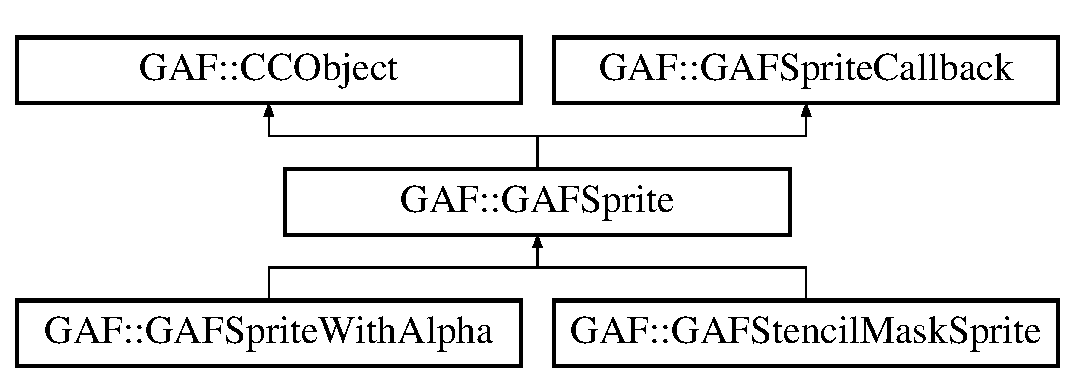
\includegraphics[height=3.000000cm]{class_g_a_f_1_1_g_a_f_sprite}
\end{center}
\end{figure}
\subsection*{Public Member Functions}
\begin{DoxyCompactItemize}
\item 
\hypertarget{class_g_a_f_1_1_g_a_f_sprite_a62060dc407edd4be0b4c8d6d2b543f51}{void {\bfseries set\-Externa\-Transform} (const \hyperlink{class_g_a_f_1_1_c_c_affine_transform}{C\-C\-Affine\-Transform} \&transform)}\label{class_g_a_f_1_1_g_a_f_sprite_a62060dc407edd4be0b4c8d6d2b543f51}

\item 
\hypertarget{class_g_a_f_1_1_g_a_f_sprite_a0964b5cbabb853fba085e618de5baa6a}{bool {\bfseries init\-With\-Texture} (void $\ast$p\-Texture, const \hyperlink{class_g_a_f_1_1_c_c_rect}{C\-C\-Rect} \&rect, bool rotated)}\label{class_g_a_f_1_1_g_a_f_sprite_a0964b5cbabb853fba085e618de5baa6a}

\item 
void $\ast$ \hyperlink{class_g_a_f_1_1_g_a_f_sprite_a06cbb88c161385cf028fef400d320f0d}{get\-External\-Pointer} ()
\item 
void \hyperlink{class_g_a_f_1_1_g_a_f_sprite_a7ef1c87d7a159fa3c29fb17c7c481cd0}{set\-External\-Pointer} (void $\ast$pointer)
\item 
\hypertarget{class_g_a_f_1_1_g_a_f_sprite_a337ff41163681341626078f0b20d5eb2}{void \hyperlink{class_g_a_f_1_1_g_a_f_sprite_a337ff41163681341626078f0b20d5eb2}{set\-Visible} (bool visible)}\label{class_g_a_f_1_1_g_a_f_sprite_a337ff41163681341626078f0b20d5eb2}

\begin{DoxyCompactList}\small\item\em set visibilty of the sprite \end{DoxyCompactList}\item 
\hypertarget{class_g_a_f_1_1_g_a_f_sprite_a7d10ff68ee86a4d7efa2a117bde8386c}{virtual void {\bfseries init\-External} ()}\label{class_g_a_f_1_1_g_a_f_sprite_a7d10ff68ee86a4d7efa2a117bde8386c}

\item 
\hypertarget{class_g_a_f_1_1_g_a_f_sprite_a5acd185b3e1e531b1d43b58253852c50}{void {\bfseries get\-Parameter} (int parameter, void $\ast$result)}\label{class_g_a_f_1_1_g_a_f_sprite_a5acd185b3e1e531b1d43b58253852c50}

\end{DoxyCompactItemize}
\subsection*{Public Attributes}
\begin{DoxyCompactItemize}
\item 
\hypertarget{class_g_a_f_1_1_g_a_f_sprite_a3bdfe86142a3ebc48942f1736ced9b21}{std\-::string \hyperlink{class_g_a_f_1_1_g_a_f_sprite_a3bdfe86142a3ebc48942f1736ced9b21}{object\-Id}}\label{class_g_a_f_1_1_g_a_f_sprite_a3bdfe86142a3ebc48942f1736ced9b21}

\begin{DoxyCompactList}\small\item\em object identifier found in J\-S\-O\-N \end{DoxyCompactList}\end{DoxyCompactItemize}


\subsection{Detailed Description}
This is utility class used by G\-A\-F playback. It does not perform rendering or use Open\-G\-L. Instead, it references backend object via \hyperlink{class_g_a_f_1_1_g_a_f_sprite_a06cbb88c161385cf028fef400d320f0d}{G\-A\-F\-Sprite\-::get\-External\-Pointer}. 

\subsection{Member Function Documentation}
\hypertarget{class_g_a_f_1_1_g_a_f_sprite_a06cbb88c161385cf028fef400d320f0d}{\index{G\-A\-F\-::\-G\-A\-F\-Sprite@{G\-A\-F\-::\-G\-A\-F\-Sprite}!get\-External\-Pointer@{get\-External\-Pointer}}
\index{get\-External\-Pointer@{get\-External\-Pointer}!GAF::GAFSprite@{G\-A\-F\-::\-G\-A\-F\-Sprite}}
\subsubsection[{get\-External\-Pointer}]{\setlength{\rightskip}{0pt plus 5cm}void$\ast$ G\-A\-F\-::\-G\-A\-F\-Sprite\-::get\-External\-Pointer (
\begin{DoxyParamCaption}
{}
\end{DoxyParamCaption}
)\hspace{0.3cm}{\ttfamily [inline]}}}\label{class_g_a_f_1_1_g_a_f_sprite_a06cbb88c161385cf028fef400d320f0d}
\begin{DoxyReturn}{Returns}
external pointer to G\-A\-F rendering backend object 
\end{DoxyReturn}
\hypertarget{class_g_a_f_1_1_g_a_f_sprite_a7ef1c87d7a159fa3c29fb17c7c481cd0}{\index{G\-A\-F\-::\-G\-A\-F\-Sprite@{G\-A\-F\-::\-G\-A\-F\-Sprite}!set\-External\-Pointer@{set\-External\-Pointer}}
\index{set\-External\-Pointer@{set\-External\-Pointer}!GAF::GAFSprite@{G\-A\-F\-::\-G\-A\-F\-Sprite}}
\subsubsection[{set\-External\-Pointer}]{\setlength{\rightskip}{0pt plus 5cm}void G\-A\-F\-::\-G\-A\-F\-Sprite\-::set\-External\-Pointer (
\begin{DoxyParamCaption}
\item[{void $\ast$}]{pointer}
\end{DoxyParamCaption}
)\hspace{0.3cm}{\ttfamily [inline]}}}\label{class_g_a_f_1_1_g_a_f_sprite_a7ef1c87d7a159fa3c29fb17c7c481cd0}

\begin{DoxyParams}{Parameters}
{\em pointer} & -\/ external pointer to G\-A\-F rendering backend object \\
\hline
\end{DoxyParams}


The documentation for this class was generated from the following file\-:\begin{DoxyCompactItemize}
\item 
G\-A\-F\-Sprite.\-h\end{DoxyCompactItemize}

\hypertarget{class_g_a_f_1_1_g_a_f_sprite_callback}{\section{G\-A\-F\-:\-:G\-A\-F\-Sprite\-Callback Class Reference}
\label{class_g_a_f_1_1_g_a_f_sprite_callback}\index{G\-A\-F\-::\-G\-A\-F\-Sprite\-Callback@{G\-A\-F\-::\-G\-A\-F\-Sprite\-Callback}}
}


{\ttfamily \#include $<$G\-A\-F\-Marmalade.\-h$>$}

Inheritance diagram for G\-A\-F\-:\-:G\-A\-F\-Sprite\-Callback\-:\begin{figure}[H]
\begin{center}
\leavevmode
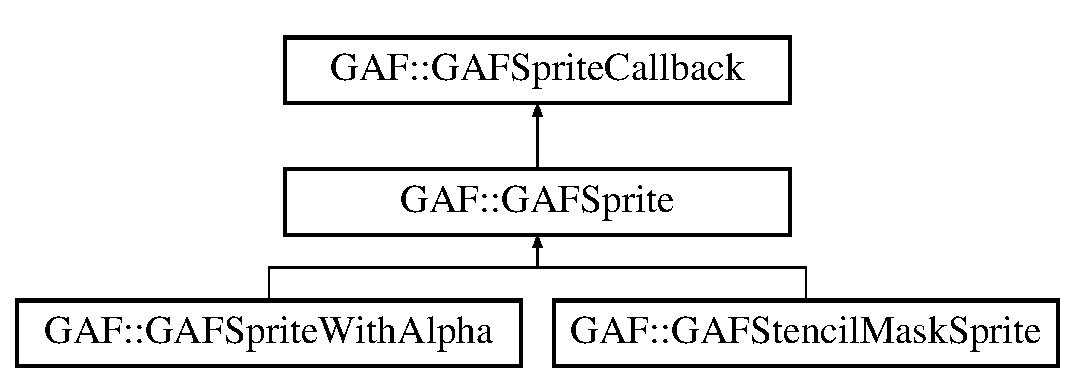
\includegraphics[height=3.000000cm]{class_g_a_f_1_1_g_a_f_sprite_callback}
\end{center}
\end{figure}
\subsection*{Public Member Functions}
\begin{DoxyCompactItemize}
\item 
\hypertarget{class_g_a_f_1_1_g_a_f_sprite_callback_a153d7fa63a377b294fa9b040f89bd6a6}{virtual void {\bfseries get\-Parameter} (int parameter, void $\ast$result)=0}\label{class_g_a_f_1_1_g_a_f_sprite_callback_a153d7fa63a377b294fa9b040f89bd6a6}

\end{DoxyCompactItemize}


\subsection{Detailed Description}
\begin{DoxyNote}{Note}
this class is used to quiry sprte parameters that have non-\/primitive data types. Now they are only shader parameters. 
\end{DoxyNote}


The documentation for this class was generated from the following file\-:\begin{DoxyCompactItemize}
\item 
G\-A\-F\-Marmalade.\-h\end{DoxyCompactItemize}

\hypertarget{class_g_a_f_1_1_g_a_f_sprite_with_alpha}{\section{G\-A\-F\-:\-:G\-A\-F\-Sprite\-With\-Alpha Class Reference}
\label{class_g_a_f_1_1_g_a_f_sprite_with_alpha}\index{G\-A\-F\-::\-G\-A\-F\-Sprite\-With\-Alpha@{G\-A\-F\-::\-G\-A\-F\-Sprite\-With\-Alpha}}
}
Inheritance diagram for G\-A\-F\-:\-:G\-A\-F\-Sprite\-With\-Alpha\-:\begin{figure}[H]
\begin{center}
\leavevmode
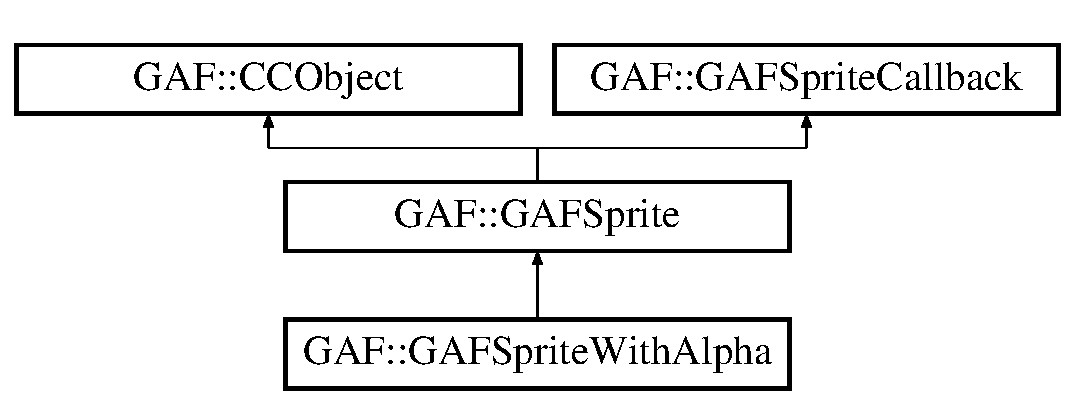
\includegraphics[height=3.000000cm]{class_g_a_f_1_1_g_a_f_sprite_with_alpha}
\end{center}
\end{figure}
\subsection*{Public Member Functions}
\begin{DoxyCompactItemize}
\item 
\hypertarget{class_g_a_f_1_1_g_a_f_sprite_with_alpha_a0ff0709d93c1b67f9065e47c87397df7}{void {\bfseries set\-Color\-Transform} (const float $\ast$mults, const float $\ast$offsets)}\label{class_g_a_f_1_1_g_a_f_sprite_with_alpha_a0ff0709d93c1b67f9065e47c87397df7}

\item 
const float $\ast$ \hyperlink{class_g_a_f_1_1_g_a_f_sprite_with_alpha_a0b03aca5ef3f81a3672ab5ccd6445d80}{get\-Color\-Transform} () const 
\item 
\hypertarget{class_g_a_f_1_1_g_a_f_sprite_with_alpha_ac56b5e2afe33626a142e8cf9f3c4abbe}{void {\bfseries init\-External} ()}\label{class_g_a_f_1_1_g_a_f_sprite_with_alpha_ac56b5e2afe33626a142e8cf9f3c4abbe}

\item 
\hypertarget{class_g_a_f_1_1_g_a_f_sprite_with_alpha_a3fbb262c8b3c4014ffae643f12cb6569}{void {\bfseries set\-Color\-Transform} (const float $\ast$color\-Transform)}\label{class_g_a_f_1_1_g_a_f_sprite_with_alpha_a3fbb262c8b3c4014ffae643f12cb6569}

\item 
\hypertarget{class_g_a_f_1_1_g_a_f_sprite_with_alpha_a658502a8de039fe45ad50ae7da1ac8cc}{void {\bfseries set\-Blur\-Radius} (const \hyperlink{class_g_a_f_1_1_c_c_size}{C\-C\-Size} \&blur\-Radius)}\label{class_g_a_f_1_1_g_a_f_sprite_with_alpha_a658502a8de039fe45ad50ae7da1ac8cc}

\item 
\hypertarget{class_g_a_f_1_1_g_a_f_sprite_with_alpha_a438088428165e03f7392e582b69fee00}{virtual void {\bfseries get\-Parameter} (int parameter, void $\ast$result)}\label{class_g_a_f_1_1_g_a_f_sprite_with_alpha_a438088428165e03f7392e582b69fee00}

\end{DoxyCompactItemize}
\subsection*{Additional Inherited Members}


\subsection{Member Function Documentation}
\hypertarget{class_g_a_f_1_1_g_a_f_sprite_with_alpha_a0b03aca5ef3f81a3672ab5ccd6445d80}{\index{G\-A\-F\-::\-G\-A\-F\-Sprite\-With\-Alpha@{G\-A\-F\-::\-G\-A\-F\-Sprite\-With\-Alpha}!get\-Color\-Transform@{get\-Color\-Transform}}
\index{get\-Color\-Transform@{get\-Color\-Transform}!GAF::GAFSpriteWithAlpha@{G\-A\-F\-::\-G\-A\-F\-Sprite\-With\-Alpha}}
\subsubsection[{get\-Color\-Transform}]{\setlength{\rightskip}{0pt plus 5cm}const float$\ast$ G\-A\-F\-::\-G\-A\-F\-Sprite\-With\-Alpha\-::get\-Color\-Transform (
\begin{DoxyParamCaption}
{}
\end{DoxyParamCaption}
) const\hspace{0.3cm}{\ttfamily [inline]}}}\label{class_g_a_f_1_1_g_a_f_sprite_with_alpha_a0b03aca5ef3f81a3672ab5ccd6445d80}
color transform is float\mbox{[}8\mbox{]} 0-\/3 mults, 4-\/7 offsets more details here -\/ \href{http://help.adobe.com/en_US/FlashPlatform/reference/actionscript/3/flash/geom/ColorTransform.html}{\tt http\-://help.\-adobe.\-com/en\-\_\-\-U\-S/\-Flash\-Platform/reference/actionscript/3/flash/geom/\-Color\-Transform.\-html} 

The documentation for this class was generated from the following file\-:\begin{DoxyCompactItemize}
\item 
G\-A\-F\-Sprite\-With\-Alpha.\-h\end{DoxyCompactItemize}

\hypertarget{class_g_a_f_1_1_g_a_f_stencil_mask_sprite}{\section{G\-A\-F\-:\-:G\-A\-F\-Stencil\-Mask\-Sprite Class Reference}
\label{class_g_a_f_1_1_g_a_f_stencil_mask_sprite}\index{G\-A\-F\-::\-G\-A\-F\-Stencil\-Mask\-Sprite@{G\-A\-F\-::\-G\-A\-F\-Stencil\-Mask\-Sprite}}
}
Inheritance diagram for G\-A\-F\-:\-:G\-A\-F\-Stencil\-Mask\-Sprite\-:\begin{figure}[H]
\begin{center}
\leavevmode
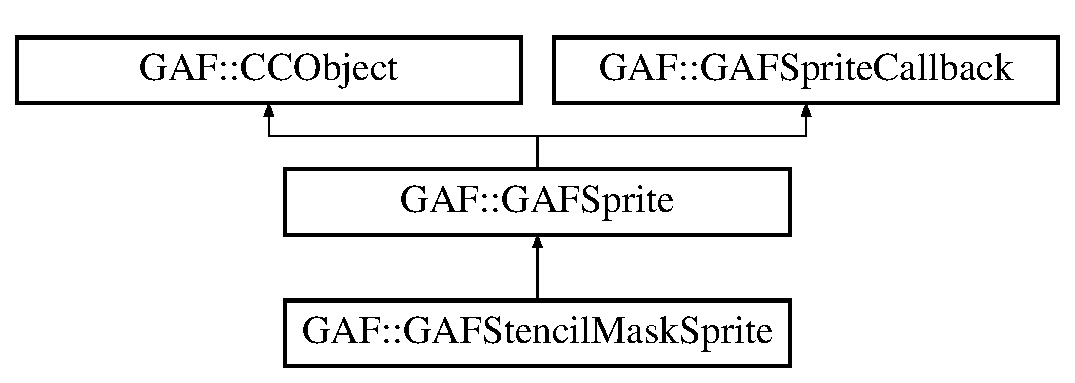
\includegraphics[height=3.000000cm]{class_g_a_f_1_1_g_a_f_stencil_mask_sprite}
\end{center}
\end{figure}
\subsection*{Public Member Functions}
\begin{DoxyCompactItemize}
\item 
\hypertarget{class_g_a_f_1_1_g_a_f_stencil_mask_sprite_a7d3ece82011b77f045c95632592b746b}{void {\bfseries add\-Masked\-Object} (\hyperlink{class_g_a_f_1_1_g_a_f_sprite}{G\-A\-F\-Sprite} $\ast$an\-Object)}\label{class_g_a_f_1_1_g_a_f_stencil_mask_sprite_a7d3ece82011b77f045c95632592b746b}

\item 
\hypertarget{class_g_a_f_1_1_g_a_f_stencil_mask_sprite_a8c6dbf171d1e6b28da266197521d03dd}{void {\bfseries init\-External} ()}\label{class_g_a_f_1_1_g_a_f_stencil_mask_sprite_a8c6dbf171d1e6b28da266197521d03dd}

\item 
\hypertarget{class_g_a_f_1_1_g_a_f_stencil_mask_sprite_afd982bb4bbf76c85f195af1d2d9fb83c}{void {\bfseries get\-Parameter} (int parameter, void $\ast$result)}\label{class_g_a_f_1_1_g_a_f_stencil_mask_sprite_afd982bb4bbf76c85f195af1d2d9fb83c}

\end{DoxyCompactItemize}
\subsection*{Static Public Member Functions}
\begin{DoxyCompactItemize}
\item 
\hypertarget{class_g_a_f_1_1_g_a_f_stencil_mask_sprite_a758c3751f5e9d5bc8be38d670d2199df}{static void {\bfseries update\-Mask\-Container\-Of} (\hyperlink{class_g_a_f_1_1_g_a_f_sprite}{G\-A\-F\-Sprite} $\ast$node)}\label{class_g_a_f_1_1_g_a_f_stencil_mask_sprite_a758c3751f5e9d5bc8be38d670d2199df}

\end{DoxyCompactItemize}
\subsection*{Additional Inherited Members}


The documentation for this class was generated from the following file\-:\begin{DoxyCompactItemize}
\item 
G\-A\-F\-Stencil\-Mask\-Sprite.\-h\end{DoxyCompactItemize}

\hypertarget{class_g_a_f_1_1_g_a_f_subobject_state}{\section{G\-A\-F\-:\-:G\-A\-F\-Subobject\-State Class Reference}
\label{class_g_a_f_1_1_g_a_f_subobject_state}\index{G\-A\-F\-::\-G\-A\-F\-Subobject\-State@{G\-A\-F\-::\-G\-A\-F\-Subobject\-State}}
}
Inheritance diagram for G\-A\-F\-:\-:G\-A\-F\-Subobject\-State\-:\begin{figure}[H]
\begin{center}
\leavevmode
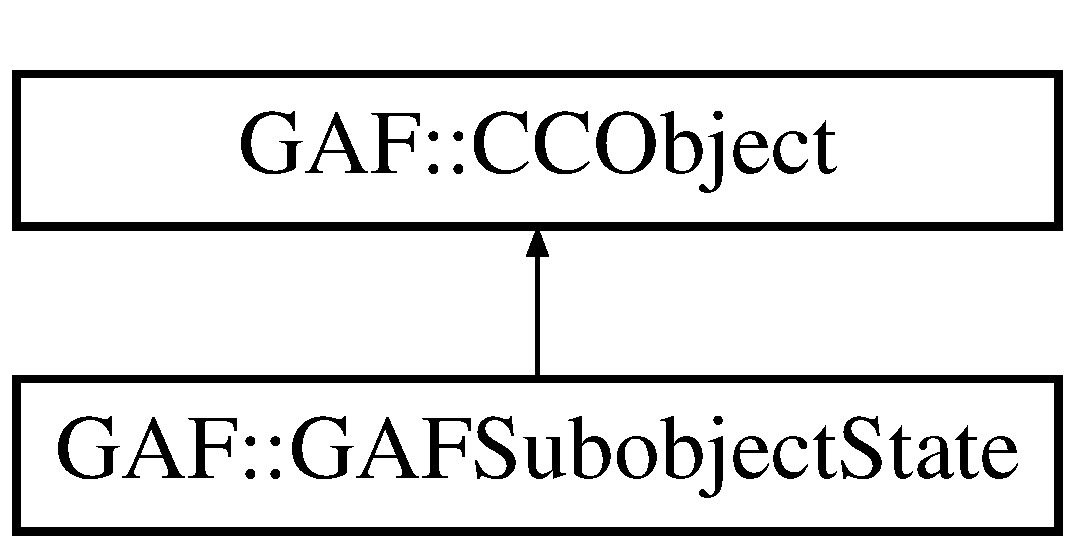
\includegraphics[height=2.000000cm]{class_g_a_f_1_1_g_a_f_subobject_state}
\end{center}
\end{figure}
\subsection*{Public Member Functions}
\begin{DoxyCompactItemize}
\item 
\hypertarget{class_g_a_f_1_1_g_a_f_subobject_state_ae5f69c2547384b4b1599eedf36cd6821}{bool {\bfseries init\-With\-State\-Dictionary} (\hyperlink{class_g_a_f_1_1_c_c_dictionary}{C\-C\-Dictionary} $\ast$dict, const char $\ast$object\-Id)}\label{class_g_a_f_1_1_g_a_f_subobject_state_ae5f69c2547384b4b1599eedf36cd6821}

\item 
\hypertarget{class_g_a_f_1_1_g_a_f_subobject_state_a8a9711a7df7a1211e8502b997de314d2}{bool {\bfseries init\-Empty\-Winth\-Object\-Id} (const char $\ast$object\-Id)}\label{class_g_a_f_1_1_g_a_f_subobject_state_a8a9711a7df7a1211e8502b997de314d2}

\item 
\hypertarget{class_g_a_f_1_1_g_a_f_subobject_state_a572cb5d24227630b969e9b12c8a8c1c9}{\hyperlink{class_g_a_f_1_1_c_c_dictionary}{C\-C\-Dictionary} $\ast$ {\bfseries filters} ()}\label{class_g_a_f_1_1_g_a_f_subobject_state_a572cb5d24227630b969e9b12c8a8c1c9}

\item 
\hypertarget{class_g_a_f_1_1_g_a_f_subobject_state_ae40fb62651bfeed23b670abd0a21a962}{float $\ast$ {\bfseries color\-Mults} ()}\label{class_g_a_f_1_1_g_a_f_subobject_state_ae40fb62651bfeed23b670abd0a21a962}

\item 
\hypertarget{class_g_a_f_1_1_g_a_f_subobject_state_a2ac1e9465fddc6cac9223506644484d1}{float $\ast$ {\bfseries color\-Offsets} ()}\label{class_g_a_f_1_1_g_a_f_subobject_state_a2ac1e9465fddc6cac9223506644484d1}

\item 
\hypertarget{class_g_a_f_1_1_g_a_f_subobject_state_ad481472523fdf6f2d4881445039f5ea7}{bool {\bfseries is\-Visisble} () const }\label{class_g_a_f_1_1_g_a_f_subobject_state_ad481472523fdf6f2d4881445039f5ea7}

\end{DoxyCompactItemize}
\subsection*{Static Public Member Functions}
\begin{DoxyCompactItemize}
\item 
\hypertarget{class_g_a_f_1_1_g_a_f_subobject_state_abf01d75392777d5042ef902a6e8d424d}{static \hyperlink{class_g_a_f_1_1_g_a_f_subobject_state}{G\-A\-F\-Subobject\-State} $\ast$ {\bfseries create\-With\-State\-Dictionary} (\hyperlink{class_g_a_f_1_1_c_c_dictionary}{C\-C\-Dictionary} $\ast$dict, const char $\ast$object\-Id)}\label{class_g_a_f_1_1_g_a_f_subobject_state_abf01d75392777d5042ef902a6e8d424d}

\item 
\hypertarget{class_g_a_f_1_1_g_a_f_subobject_state_aa75f07b37f8e3cd36b35f0ec404c25f6}{static \hyperlink{class_g_a_f_1_1_g_a_f_subobject_state}{G\-A\-F\-Subobject\-State} $\ast$ {\bfseries create\-Empty\-With\-Object\-Id} (const char $\ast$object\-Id)}\label{class_g_a_f_1_1_g_a_f_subobject_state_aa75f07b37f8e3cd36b35f0ec404c25f6}

\end{DoxyCompactItemize}
\subsection*{Public Attributes}
\begin{DoxyCompactItemize}
\item 
\hypertarget{class_g_a_f_1_1_g_a_f_subobject_state_ad0d50c5a7e6b321a72bbf24dbf6199dd}{std\-::string {\bfseries object\-Id}}\label{class_g_a_f_1_1_g_a_f_subobject_state_ad0d50c5a7e6b321a72bbf24dbf6199dd}

\item 
\hypertarget{class_g_a_f_1_1_g_a_f_subobject_state_aec77797540e84579a64373a032abc234}{int {\bfseries z\-Index}}\label{class_g_a_f_1_1_g_a_f_subobject_state_aec77797540e84579a64373a032abc234}

\item 
\hypertarget{class_g_a_f_1_1_g_a_f_subobject_state_a083db321fc5887ef866e946e5807c6c6}{std\-::string {\bfseries mask\-Object\-Id}}\label{class_g_a_f_1_1_g_a_f_subobject_state_a083db321fc5887ef866e946e5807c6c6}

\item 
\hypertarget{class_g_a_f_1_1_g_a_f_subobject_state_aa2102cfe9627c7ac880063f303066229}{\hyperlink{class_g_a_f_1_1_c_c_affine_transform}{C\-C\-Affine\-Transform} {\bfseries affine\-Transform}}\label{class_g_a_f_1_1_g_a_f_subobject_state_aa2102cfe9627c7ac880063f303066229}

\end{DoxyCompactItemize}


The documentation for this class was generated from the following file\-:\begin{DoxyCompactItemize}
\item 
G\-A\-F\-Subobject\-State.\-h\end{DoxyCompactItemize}

\hypertarget{class_g_a_f_1_1_g_a_f_texture_atlas}{\section{G\-A\-F\-:\-:G\-A\-F\-Texture\-Atlas Class Reference}
\label{class_g_a_f_1_1_g_a_f_texture_atlas}\index{G\-A\-F\-::\-G\-A\-F\-Texture\-Atlas@{G\-A\-F\-::\-G\-A\-F\-Texture\-Atlas}}
}
Inheritance diagram for G\-A\-F\-:\-:G\-A\-F\-Texture\-Atlas\-:\begin{figure}[H]
\begin{center}
\leavevmode
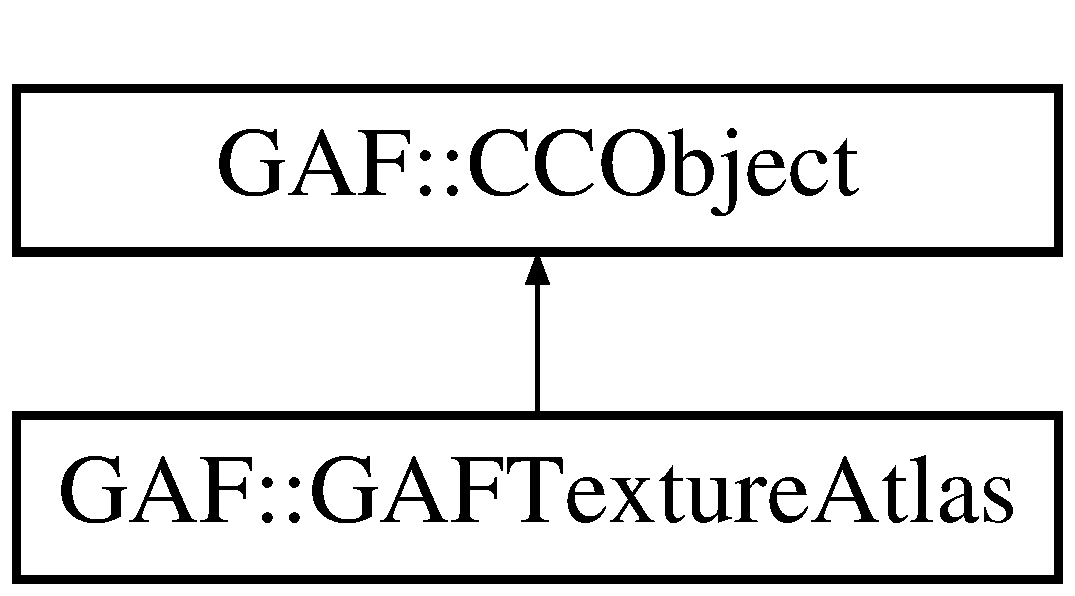
\includegraphics[height=2.000000cm]{class_g_a_f_1_1_g_a_f_texture_atlas}
\end{center}
\end{figure}
\subsection*{Public Member Functions}
\begin{DoxyCompactItemize}
\item 
\hypertarget{class_g_a_f_1_1_g_a_f_texture_atlas_ad0e9c9b7d9ed9fedb4f77ec2f9a754f2}{bool {\bfseries init} (const char $\ast$a\-Textures\-Directory, \hyperlink{class_g_a_f_1_1_c_c_dictionary}{C\-C\-Dictionary} $\ast$a\-Texture\-Atlas\-Config\-Dictionary)}\label{class_g_a_f_1_1_g_a_f_texture_atlas_ad0e9c9b7d9ed9fedb4f77ec2f9a754f2}

\item 
\hypertarget{class_g_a_f_1_1_g_a_f_texture_atlas_ad079217d4bc03bfa5a1be2f23955d508}{bool {\bfseries loaded} () const }\label{class_g_a_f_1_1_g_a_f_texture_atlas_ad079217d4bc03bfa5a1be2f23955d508}

\item 
\hypertarget{class_g_a_f_1_1_g_a_f_texture_atlas_a1d4a6fa2bd1eef23417c46de6e92a1dc}{\hyperlink{class_g_a_f_1_1_c_c_image}{C\-C\-Image} $\ast$ {\bfseries image} ()}\label{class_g_a_f_1_1_g_a_f_texture_atlas_a1d4a6fa2bd1eef23417c46de6e92a1dc}

\item 
\hypertarget{class_g_a_f_1_1_g_a_f_texture_atlas_a1a5dccdaf8fa3721667d9dfecbbb5fba}{\hyperlink{class_g_a_f_1_1_c_c_array}{C\-C\-Array} $\ast$ {\bfseries images} ()}\label{class_g_a_f_1_1_g_a_f_texture_atlas_a1a5dccdaf8fa3721667d9dfecbbb5fba}

\item 
\hypertarget{class_g_a_f_1_1_g_a_f_texture_atlas_a23a8bb9096effdd4c298c488b4edc6a1}{\hyperlink{class_g_a_f_1_1_c_c_texture2_d}{C\-C\-Texture2\-D} $\ast$ {\bfseries texture} ()}\label{class_g_a_f_1_1_g_a_f_texture_atlas_a23a8bb9096effdd4c298c488b4edc6a1}

\item 
\hypertarget{class_g_a_f_1_1_g_a_f_texture_atlas_a6a2e81d603ea4cb5ccb28c70c3d2ac08}{\hyperlink{class_g_a_f_1_1_c_c_array}{C\-C\-Array} $\ast$ {\bfseries textures} ()}\label{class_g_a_f_1_1_g_a_f_texture_atlas_a6a2e81d603ea4cb5ccb28c70c3d2ac08}

\item 
\hypertarget{class_g_a_f_1_1_g_a_f_texture_atlas_a48e769c7aa5854840b3c076bdb1a7380}{\hyperlink{class_g_a_f_1_1_c_c_dictionary}{C\-C\-Dictionary} $\ast$ {\bfseries elements} ()}\label{class_g_a_f_1_1_g_a_f_texture_atlas_a48e769c7aa5854840b3c076bdb1a7380}

\item 
\hypertarget{class_g_a_f_1_1_g_a_f_texture_atlas_aee1e3f16c47352358e5f23258b23cc23}{bool {\bfseries load\-Elements\-From\-Animation\-Config\-Dictionary} (\hyperlink{class_g_a_f_1_1_c_c_dictionary}{C\-C\-Dictionary} $\ast$a\-Config\-Dictionary)}\label{class_g_a_f_1_1_g_a_f_texture_atlas_aee1e3f16c47352358e5f23258b23cc23}

\end{DoxyCompactItemize}
\subsection*{Static Public Member Functions}
\begin{DoxyCompactItemize}
\item 
\hypertarget{class_g_a_f_1_1_g_a_f_texture_atlas_a52a21a062a5b52719eda910c3f335070}{static \hyperlink{class_g_a_f_1_1_g_a_f_texture_atlas}{G\-A\-F\-Texture\-Atlas} $\ast$ {\bfseries create} (const char $\ast$a\-Textures\-Directory, \hyperlink{class_g_a_f_1_1_c_c_dictionary}{C\-C\-Dictionary} $\ast$a\-Texture\-Atlas\-Config\-Dictionary)}\label{class_g_a_f_1_1_g_a_f_texture_atlas_a52a21a062a5b52719eda910c3f335070}

\end{DoxyCompactItemize}


The documentation for this class was generated from the following file\-:\begin{DoxyCompactItemize}
\item 
G\-A\-F\-Texture\-Atlas.\-h\end{DoxyCompactItemize}

\hypertarget{class_g_a_f_1_1_g_a_f_texture_atlas_element}{\section{G\-A\-F\-:\-:G\-A\-F\-Texture\-Atlas\-Element Class Reference}
\label{class_g_a_f_1_1_g_a_f_texture_atlas_element}\index{G\-A\-F\-::\-G\-A\-F\-Texture\-Atlas\-Element@{G\-A\-F\-::\-G\-A\-F\-Texture\-Atlas\-Element}}
}
Inheritance diagram for G\-A\-F\-:\-:G\-A\-F\-Texture\-Atlas\-Element\-:\begin{figure}[H]
\begin{center}
\leavevmode
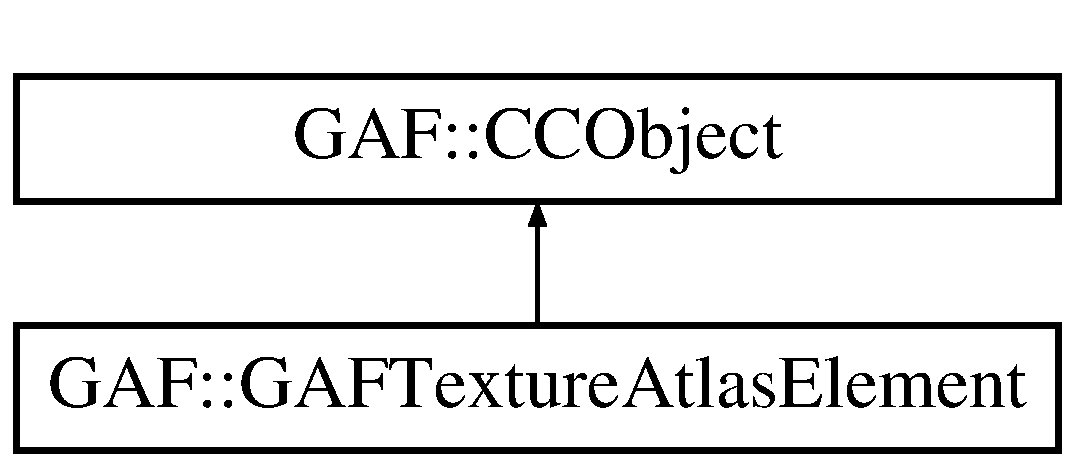
\includegraphics[height=2.000000cm]{class_g_a_f_1_1_g_a_f_texture_atlas_element}
\end{center}
\end{figure}
\subsection*{Public Member Functions}
\begin{DoxyCompactItemize}
\item 
\hypertarget{class_g_a_f_1_1_g_a_f_texture_atlas_element_ace1051e2a8d8a2640b75970bc6ee3499}{bool {\bfseries init\-With\-Dictionary} (\hyperlink{class_g_a_f_1_1_c_c_dictionary}{C\-C\-Dictionary} $\ast$a\-Dictionary)}\label{class_g_a_f_1_1_g_a_f_texture_atlas_element_ace1051e2a8d8a2640b75970bc6ee3499}

\end{DoxyCompactItemize}
\subsection*{Static Public Member Functions}
\begin{DoxyCompactItemize}
\item 
\hypertarget{class_g_a_f_1_1_g_a_f_texture_atlas_element_af3b864b9aea64b04dff34b076dec085a}{static \hyperlink{class_g_a_f_1_1_g_a_f_texture_atlas_element}{G\-A\-F\-Texture\-Atlas\-Element} $\ast$ {\bfseries create} (\hyperlink{class_g_a_f_1_1_c_c_dictionary}{C\-C\-Dictionary} $\ast$a\-Dictionary)}\label{class_g_a_f_1_1_g_a_f_texture_atlas_element_af3b864b9aea64b04dff34b076dec085a}

\end{DoxyCompactItemize}
\subsection*{Public Attributes}
\begin{DoxyCompactItemize}
\item 
\hypertarget{class_g_a_f_1_1_g_a_f_texture_atlas_element_a217bca4bac88f8831fba1390c5b4b956}{std\-::string {\bfseries name}}\label{class_g_a_f_1_1_g_a_f_texture_atlas_element_a217bca4bac88f8831fba1390c5b4b956}

\item 
\hypertarget{class_g_a_f_1_1_g_a_f_texture_atlas_element_a8a1316509fa831388743a1711f0d9e9a}{\hyperlink{class_g_a_f_1_1_c_c_point}{C\-C\-Point} {\bfseries pivot\-Point}}\label{class_g_a_f_1_1_g_a_f_texture_atlas_element_a8a1316509fa831388743a1711f0d9e9a}

\item 
\hypertarget{class_g_a_f_1_1_g_a_f_texture_atlas_element_ae40fb8e6364450701e2e36701c9eacf6}{\hyperlink{class_g_a_f_1_1_c_c_rect}{C\-C\-Rect} {\bfseries bounds}}\label{class_g_a_f_1_1_g_a_f_texture_atlas_element_ae40fb8e6364450701e2e36701c9eacf6}

\item 
\hypertarget{class_g_a_f_1_1_g_a_f_texture_atlas_element_acc6e12d090dd67c5e5995b9e57fa491c}{float {\bfseries scale}}\label{class_g_a_f_1_1_g_a_f_texture_atlas_element_acc6e12d090dd67c5e5995b9e57fa491c}

\item 
\hypertarget{class_g_a_f_1_1_g_a_f_texture_atlas_element_a94cafb272c7ddae6981a20d0b34e6d55}{int {\bfseries atlas\-Idx}}\label{class_g_a_f_1_1_g_a_f_texture_atlas_element_a94cafb272c7ddae6981a20d0b34e6d55}

\end{DoxyCompactItemize}


The documentation for this class was generated from the following file\-:\begin{DoxyCompactItemize}
\item 
G\-A\-F\-Texture\-Atlas\-Element.\-h\end{DoxyCompactItemize}

\addcontentsline{toc}{part}{Index}
\printindex
\end{document}
